% Options for packages loaded elsewhere
\PassOptionsToPackage{unicode}{hyperref}
\PassOptionsToPackage{hyphens}{url}
\PassOptionsToPackage{dvipsnames,svgnames*,x11names*}{xcolor}
%
\documentclass[
]{book}
\usepackage{lmodern}
\usepackage{amssymb,amsmath}
\usepackage{ifxetex,ifluatex}
\ifnum 0\ifxetex 1\fi\ifluatex 1\fi=0 % if pdftex
  \usepackage[T1]{fontenc}
  \usepackage[utf8]{inputenc}
  \usepackage{textcomp} % provide euro and other symbols
\else % if luatex or xetex
  \usepackage{unicode-math}
  \defaultfontfeatures{Scale=MatchLowercase}
  \defaultfontfeatures[\rmfamily]{Ligatures=TeX,Scale=1}
\fi
% Use upquote if available, for straight quotes in verbatim environments
\IfFileExists{upquote.sty}{\usepackage{upquote}}{}
\IfFileExists{microtype.sty}{% use microtype if available
  \usepackage[]{microtype}
  \UseMicrotypeSet[protrusion]{basicmath} % disable protrusion for tt fonts
}{}
\makeatletter
\@ifundefined{KOMAClassName}{% if non-KOMA class
  \IfFileExists{parskip.sty}{%
    \usepackage{parskip}
  }{% else
    \setlength{\parindent}{0pt}
    \setlength{\parskip}{6pt plus 2pt minus 1pt}}
}{% if KOMA class
  \KOMAoptions{parskip=half}}
\makeatother
\usepackage{xcolor}
\IfFileExists{xurl.sty}{\usepackage{xurl}}{} % add URL line breaks if available
\IfFileExists{bookmark.sty}{\usepackage{bookmark}}{\usepackage{hyperref}}
\hypersetup{
  pdftitle={Introductory Statistics with R tidyverse},
  pdfauthor={Fan Wang},
  colorlinks=true,
  linkcolor=Maroon,
  filecolor=Maroon,
  citecolor=Blue,
  urlcolor=blue,
  pdfcreator={LaTeX via pandoc}}
\urlstyle{same} % disable monospaced font for URLs
\usepackage{color}
\usepackage{fancyvrb}
\newcommand{\VerbBar}{|}
\newcommand{\VERB}{\Verb[commandchars=\\\{\}]}
\DefineVerbatimEnvironment{Highlighting}{Verbatim}{commandchars=\\\{\}}
% Add ',fontsize=\small' for more characters per line
\usepackage{framed}
\definecolor{shadecolor}{RGB}{248,248,248}
\newenvironment{Shaded}{\begin{snugshade}}{\end{snugshade}}
\newcommand{\AlertTok}[1]{\textcolor[rgb]{0.94,0.16,0.16}{#1}}
\newcommand{\AnnotationTok}[1]{\textcolor[rgb]{0.56,0.35,0.01}{\textbf{\textit{#1}}}}
\newcommand{\AttributeTok}[1]{\textcolor[rgb]{0.77,0.63,0.00}{#1}}
\newcommand{\BaseNTok}[1]{\textcolor[rgb]{0.00,0.00,0.81}{#1}}
\newcommand{\BuiltInTok}[1]{#1}
\newcommand{\CharTok}[1]{\textcolor[rgb]{0.31,0.60,0.02}{#1}}
\newcommand{\CommentTok}[1]{\textcolor[rgb]{0.56,0.35,0.01}{\textit{#1}}}
\newcommand{\CommentVarTok}[1]{\textcolor[rgb]{0.56,0.35,0.01}{\textbf{\textit{#1}}}}
\newcommand{\ConstantTok}[1]{\textcolor[rgb]{0.00,0.00,0.00}{#1}}
\newcommand{\ControlFlowTok}[1]{\textcolor[rgb]{0.13,0.29,0.53}{\textbf{#1}}}
\newcommand{\DataTypeTok}[1]{\textcolor[rgb]{0.13,0.29,0.53}{#1}}
\newcommand{\DecValTok}[1]{\textcolor[rgb]{0.00,0.00,0.81}{#1}}
\newcommand{\DocumentationTok}[1]{\textcolor[rgb]{0.56,0.35,0.01}{\textbf{\textit{#1}}}}
\newcommand{\ErrorTok}[1]{\textcolor[rgb]{0.64,0.00,0.00}{\textbf{#1}}}
\newcommand{\ExtensionTok}[1]{#1}
\newcommand{\FloatTok}[1]{\textcolor[rgb]{0.00,0.00,0.81}{#1}}
\newcommand{\FunctionTok}[1]{\textcolor[rgb]{0.00,0.00,0.00}{#1}}
\newcommand{\ImportTok}[1]{#1}
\newcommand{\InformationTok}[1]{\textcolor[rgb]{0.56,0.35,0.01}{\textbf{\textit{#1}}}}
\newcommand{\KeywordTok}[1]{\textcolor[rgb]{0.13,0.29,0.53}{\textbf{#1}}}
\newcommand{\NormalTok}[1]{#1}
\newcommand{\OperatorTok}[1]{\textcolor[rgb]{0.81,0.36,0.00}{\textbf{#1}}}
\newcommand{\OtherTok}[1]{\textcolor[rgb]{0.56,0.35,0.01}{#1}}
\newcommand{\PreprocessorTok}[1]{\textcolor[rgb]{0.56,0.35,0.01}{\textit{#1}}}
\newcommand{\RegionMarkerTok}[1]{#1}
\newcommand{\SpecialCharTok}[1]{\textcolor[rgb]{0.00,0.00,0.00}{#1}}
\newcommand{\SpecialStringTok}[1]{\textcolor[rgb]{0.31,0.60,0.02}{#1}}
\newcommand{\StringTok}[1]{\textcolor[rgb]{0.31,0.60,0.02}{#1}}
\newcommand{\VariableTok}[1]{\textcolor[rgb]{0.00,0.00,0.00}{#1}}
\newcommand{\VerbatimStringTok}[1]{\textcolor[rgb]{0.31,0.60,0.02}{#1}}
\newcommand{\WarningTok}[1]{\textcolor[rgb]{0.56,0.35,0.01}{\textbf{\textit{#1}}}}
\usepackage{longtable,booktabs}
% Correct order of tables after \paragraph or \subparagraph
\usepackage{etoolbox}
\makeatletter
\patchcmd\longtable{\par}{\if@noskipsec\mbox{}\fi\par}{}{}
\makeatother
% Allow footnotes in longtable head/foot
\IfFileExists{footnotehyper.sty}{\usepackage{footnotehyper}}{\usepackage{footnote}}
\makesavenoteenv{longtable}
\usepackage{graphicx}
\makeatletter
\def\maxwidth{\ifdim\Gin@nat@width>\linewidth\linewidth\else\Gin@nat@width\fi}
\def\maxheight{\ifdim\Gin@nat@height>\textheight\textheight\else\Gin@nat@height\fi}
\makeatother
% Scale images if necessary, so that they will not overflow the page
% margins by default, and it is still possible to overwrite the defaults
% using explicit options in \includegraphics[width, height, ...]{}
\setkeys{Gin}{width=\maxwidth,height=\maxheight,keepaspectratio}
% Set default figure placement to htbp
\makeatletter
\def\fps@figure{htbp}
\makeatother
\setlength{\emergencystretch}{3em} % prevent overfull lines
\providecommand{\tightlist}{%
  \setlength{\itemsep}{0pt}\setlength{\parskip}{0pt}}
\setcounter{secnumdepth}{5}
\usepackage{bbm}
\usepackage{booktabs}
\usepackage{longtable}
\usepackage{array}
\usepackage{multirow}
\usepackage{wrapfig}
\usepackage{float}
% \floatplacement{figure}{H}
\usepackage[labelformat = empty]{caption}
\usepackage{colortbl}
\usepackage{pdflscape}
\usepackage{tabu}
\usepackage{threeparttable}
\usepackage{threeparttablex}
\usepackage[normalem]{ulem}
\usepackage{makecell}
\usepackage{xcolor}
\usepackage{geometry}
\geometry{
	a4paper,
	left=1.0in,
	right=1.0in,
	top=1.0in,
	bottom=1.0in,
}
\setcounter{secnumdepth}{5}
\setcounter{tocdepth}{5}
\usepackage[]{natbib}
\bibliographystyle{apalike}

\title{Introductory Statistics with R tidyverse}
\author{Fan Wang}
\date{2020-05-16}

\begin{document}
\maketitle

{
\hypersetup{linkcolor=}
\setcounter{tocdepth}{1}
\tableofcontents
}
\hypertarget{preface}{%
\chapter*{Preface}\label{preface}}
\addcontentsline{toc}{chapter}{Preface}

This is a work-in-progress \href{https://fanwangecon.github.io/Stat4Econ/}{course website} for Introductory Statistics for Undergraduate Students, produced by \href{https://fanwangecon.github.io/}{Fan}. Course covers a limited subset of topics from \emph{Statistics for Business and Economics} (Anderson Sweeney Williams Camm Cochran 12e).

R is used. Packages from \href{https://www.tidyverse.org/}{Tidyverse} \citep{R-tidyverse} are used, including \href{https://tibble.tidyverse.org/}{tibble} \citep{R-tibble} for framing data, \href{https://dplyr.tidyverse.org/}{tidyr} \citep{R-tidyr} and \href{https://dplyr.tidyverse.org/}{dplyr} \citep{R-dplyr} for reshaping data and aggregating statistics, \href{https://ggplot2.tidyverse.org/}{ggplot2} \citep{R-ggplot2} for graphing, and \href{https://readr.tidyverse.org/}{readr} \citep{R-readr} for file reading and writing. Materials are presented as R, RMD, PDF and HTML files. To obtain all codes and raw files, see \href{https://fanwangecon.github.io/Stat4Econ/docs/gitsetup.html}{here} for github set up. For HTML files, click on the links below.

From \href{https://fanwangecon.github.io/}{Fan}'s other repositories: For dynamic borrowing and savings problems, see \href{https://fanwangecon.github.io/CodeDynaAsset/}{Dynamic Asset Repository}; For code examples, see also \href{https://fanwangecon.github.io/R4Econ/}{R Example Code}, \href{https://fanwangecon.github.io/M4Econ/}{Matlab Example Code}, and \href{https://fanwangecon.github.io/Stata4Econ/}{Stata Example Code}; For intro econ with Matlab, see \href{https://fanwangecon.github.io/Math4Econ/}{Intro Mathematics for Economists}. See \href{https://github.com/FanWangEcon}{here} for all of \href{https://fanwangecon.github.io/}{Fan}'s public repositories.

The site is built using \href{https://bookdown.org/}{Bookdown} \citep{R-bookdown}.

Please contact \href{https://fanwangecon.github.io/}{FanWangEcon} for issues or problems.

\hypertarget{survey}{%
\chapter{Survey}\label{survey}}

\hypertarget{generate-a-dataset-in-r}{%
\section{Generate A Dataset in R}\label{generate-a-dataset-in-r}}

\begin{quote}
Go back to \href{http://fanwangecon.github.io/}{fan}'s \href{https://fanwangecon.github.io/REconTools/}{REconTools} Package, \href{https://fanwangecon.github.io/R4Econ/}{R Code Examples} Repository (\href{https://fanwangecon.github.io/R4Econ/bookdown}{bookdown site}), or \href{https://fanwangecon.github.io/Stat4Econ/}{Intro Stats with R} Repository (\href{https://fanwangecon.github.io/Stat4Econ/bookdown}{bookdown site}).
\end{quote}

R has a Variety of built-in small datasets for you to experiment with, for example, opening up R, you can just type in: mtcars, and that will show you some variables and observations. The command below shows the first 5 rows of dataset \textbf{mtcars}:

\begin{Shaded}
\begin{Highlighting}[]
\KeywordTok{head}\NormalTok{(mtcars, }\DecValTok{5}\NormalTok{)}
\end{Highlighting}
\end{Shaded}

There are 52 students in a class. I am interested in how many of you go to games at the University, and how many years each of you has lived in the city of Houston. But I do not have time to ask each of you questions.

\begin{itemize}
\tightlist
\item
  My population is all 52 students in the class.
\item
  Given my limited time and resources, I will gather a sample of just 10 students.
\end{itemize}

Gathering information regarding game attendance for the 10 students, I can perhaps gain some insights about the population.

\hypertarget{a-random-sample-of-students-in-class}{%
\subsection{A Random Sample of Students in Class}\label{a-random-sample-of-students-in-class}}

I can point and pick ten random people, but how do I know I am choosing/selecting randomly? In general, we want to pick a random sample from the population. You don't want your sample of 10 to just be students in the first row or students who happen to be giving eye contacts. We want a random sample that hopefully gives us some representative information about the population of 52 students.

How do you pick random numbers?

Siri, Alexa, Google, \ldots, you can get random numbers very easily now. You can download various apps also that allows you to draw a random integer from say between 1 to 4, with an equal chance of drawing any of the four numbers.

In our class:
- we have 4 rows of seats
- we have 13 columns of seats
- there are 52 students in the class together. I will now randomly pick between 1 and 4, 10 times, and randomly pick between 1 and 13 also 10 times.

This gives me ten pairs of row and columns numbers, and these indicate which ten students will be a part of a randomly drawn sample of students.

\begin{Shaded}
\begin{Highlighting}[]
\CommentTok{\# Setting seed means we will get the same set of random numbers each time}
\KeywordTok{set.seed}\NormalTok{(}\DecValTok{12345}\NormalTok{)}
\CommentTok{\# in R, draw integers between 1 and 4, 10 times}
\NormalTok{ROW.RAND.DRAWS =}\StringTok{ }\KeywordTok{sample}\NormalTok{(}\DecValTok{1}\OperatorTok{:}\DecValTok{4}\NormalTok{, }\DecValTok{10}\NormalTok{, }\DataTypeTok{replace =} \OtherTok{TRUE}\NormalTok{)}
\CommentTok{\# in R, draw integers between 1 and 13, 10 times}
\NormalTok{COL.RAND.DRAWS =}\StringTok{ }\KeywordTok{sample}\NormalTok{(}\DecValTok{1}\OperatorTok{:}\DecValTok{13}\NormalTok{, }\DecValTok{10}\NormalTok{, }\DataTypeTok{replace =} \OtherTok{TRUE}\NormalTok{)}
\CommentTok{\# Note that the way we are drawing randomly, we could draw the same individual twice.}
\KeywordTok{rbind}\NormalTok{(ROW.RAND.DRAWS, COL.RAND.DRAWS)}
\end{Highlighting}
\end{Shaded}

\begin{verbatim}
##                [,1] [,2] [,3] [,4] [,5] [,6] [,7] [,8] [,9] [,10]
## ROW.RAND.DRAWS    2    3    4    2    4    4    2    1    3     4
## COL.RAND.DRAWS    8    2    6   11    6    7   10    1    8     7
\end{verbatim}

\hypertarget{create-the-dataset-row-by-row}{%
\subsubsection{Create the Dataset Row by Row}\label{create-the-dataset-row-by-row}}

R has \emph{base} packages. Many of R's best packages do not come with the base packages. You have to install separately. One of the best packages for data science is \href{https://www.tidyverse.org/}{tidyverse}. \textbf{tidyverse} has a great package called \href{https://tibble.tidyverse.org/}{tibble}, which is a great way to deal with what are called dataframes, where we store our data. \textbf{tidyverse} also has \href{https://dplyr.tidyverse.org/}{dplyr}, which is a powerful set of tools for transforming data.

Sequentially, in class, we ask each of the 10 randomly drawn students a number of questions, and record the answers in the dataframe.

\begin{Shaded}
\begin{Highlighting}[]
\NormalTok{df \textless{}{-}}\StringTok{ }\KeywordTok{tibble}\NormalTok{(}\DataTypeTok{ID =} \KeywordTok{integer}\NormalTok{(), }\DataTypeTok{ROW =} \KeywordTok{integer}\NormalTok{(), }\DataTypeTok{COL =} \KeywordTok{integer}\NormalTok{(),}
             \DataTypeTok{gender =} \KeywordTok{factor}\NormalTok{(),}
             \DataTypeTok{years.in.houston =} \KeywordTok{double}\NormalTok{(),}
             \DataTypeTok{major =} \KeywordTok{factor}\NormalTok{(),}
             \DataTypeTok{commute =} \KeywordTok{factor}\NormalTok{(),}
             \DataTypeTok{games.attended =} \KeywordTok{integer}\NormalTok{())}


\CommentTok{\# Ask Students Questions and Record Answers}
\NormalTok{df \textless{}{-}}\StringTok{ }\KeywordTok{add\_row}\NormalTok{(df, }\DataTypeTok{ID=}\DecValTok{1}\NormalTok{ , }\DataTypeTok{ROW=}\DecValTok{3}\NormalTok{, }\DataTypeTok{COL=}\DecValTok{1}\NormalTok{,  }\DataTypeTok{gender=}\StringTok{\textquotesingle{}MALE\textquotesingle{}}\NormalTok{,   }\DataTypeTok{years.in.houston=}\FloatTok{21.0}\NormalTok{,}
              \DataTypeTok{major=}\StringTok{\textquotesingle{}ECON\textquotesingle{}}\NormalTok{, }\DataTypeTok{commute=}\StringTok{\textquotesingle{}YES\textquotesingle{}}\NormalTok{, }\DataTypeTok{games.attended=}\DecValTok{0}\NormalTok{)}
\NormalTok{df \textless{}{-}}\StringTok{ }\KeywordTok{add\_row}\NormalTok{(df, }\DataTypeTok{ID=}\DecValTok{2}\NormalTok{ , }\DataTypeTok{ROW=}\DecValTok{4}\NormalTok{, }\DataTypeTok{COL=}\DecValTok{2}\NormalTok{,  }\DataTypeTok{gender=}\StringTok{\textquotesingle{}FEMALE\textquotesingle{}}\NormalTok{, }\DataTypeTok{years.in.houston=}\FloatTok{21.0}\NormalTok{,}
              \DataTypeTok{major=}\StringTok{\textquotesingle{}HEALTH\textquotesingle{}}\NormalTok{, }\DataTypeTok{commute=}\StringTok{\textquotesingle{}YES\textquotesingle{}}\NormalTok{, }\DataTypeTok{games.attended=}\DecValTok{2}\NormalTok{)}
\NormalTok{df \textless{}{-}}\StringTok{ }\KeywordTok{add\_row}\NormalTok{(df, }\DataTypeTok{ID=}\DecValTok{3}\NormalTok{ , }\DataTypeTok{ROW=}\DecValTok{4}\NormalTok{, }\DataTypeTok{COL=}\DecValTok{10}\NormalTok{, }\DataTypeTok{gender=}\StringTok{\textquotesingle{}MALE\textquotesingle{}}\NormalTok{,   }\DataTypeTok{years.in.houston=}\FloatTok{22.0}\NormalTok{,}
              \DataTypeTok{major=}\StringTok{\textquotesingle{}ECON\textquotesingle{}}\NormalTok{, }\DataTypeTok{commute=}\StringTok{\textquotesingle{}YES\textquotesingle{}}\NormalTok{, }\DataTypeTok{games.attended=}\DecValTok{0}\NormalTok{)}
\NormalTok{df \textless{}{-}}\StringTok{ }\KeywordTok{add\_row}\NormalTok{(df, }\DataTypeTok{ID=}\DecValTok{4}\NormalTok{ , }\DataTypeTok{ROW=}\DecValTok{4}\NormalTok{, }\DataTypeTok{COL=}\DecValTok{1}\NormalTok{,  }\DataTypeTok{gender=}\StringTok{\textquotesingle{}MALE\textquotesingle{}}\NormalTok{,   }\DataTypeTok{years.in.houston=}\FloatTok{22.0}\NormalTok{,}
              \DataTypeTok{major=}\StringTok{\textquotesingle{}ECON\textquotesingle{}}\NormalTok{, }\DataTypeTok{commute=}\StringTok{\textquotesingle{}YES\textquotesingle{}}\NormalTok{, }\DataTypeTok{games.attended=}\DecValTok{14}\NormalTok{)}
\NormalTok{df \textless{}{-}}\StringTok{ }\KeywordTok{add\_row}\NormalTok{(df, }\DataTypeTok{ID=}\DecValTok{5}\NormalTok{ , }\DataTypeTok{ROW=}\DecValTok{2}\NormalTok{, }\DataTypeTok{COL=}\DecValTok{6}\NormalTok{,  }\DataTypeTok{gender=}\StringTok{\textquotesingle{}FEMALE\textquotesingle{}}\NormalTok{, }\DataTypeTok{years.in.houston=}\FloatTok{20.0}\NormalTok{,}
              \DataTypeTok{major=}\StringTok{\textquotesingle{}ECON\textquotesingle{}}\NormalTok{, }\DataTypeTok{commute=}\StringTok{\textquotesingle{}YES\textquotesingle{}}\NormalTok{, }\DataTypeTok{games.attended=}\DecValTok{0}\NormalTok{)}
\NormalTok{df \textless{}{-}}\StringTok{ }\KeywordTok{add\_row}\NormalTok{(df, }\DataTypeTok{ID=}\DecValTok{6}\NormalTok{ , }\DataTypeTok{ROW=}\DecValTok{1}\NormalTok{, }\DataTypeTok{COL=}\DecValTok{7}\NormalTok{,  }\DataTypeTok{gender=}\StringTok{\textquotesingle{}MALE\textquotesingle{}}\NormalTok{,   }\DataTypeTok{years.in.houston=}\FloatTok{3.0}\NormalTok{,}
              \DataTypeTok{major=}\StringTok{\textquotesingle{}PSYCH\textquotesingle{}}\NormalTok{, }\DataTypeTok{commute=}\StringTok{\textquotesingle{}YES\textquotesingle{}}\NormalTok{, }\DataTypeTok{games.attended=}\DecValTok{0}\NormalTok{)}
\NormalTok{df \textless{}{-}}\StringTok{ }\KeywordTok{add\_row}\NormalTok{(df, }\DataTypeTok{ID=}\DecValTok{7}\NormalTok{ , }\DataTypeTok{ROW=}\DecValTok{2}\NormalTok{, }\DataTypeTok{COL=}\DecValTok{6}\NormalTok{,  }\DataTypeTok{gender=}\StringTok{\textquotesingle{}MALE\textquotesingle{}}\NormalTok{,   }\DataTypeTok{years.in.houston=}\FloatTok{25.0}\NormalTok{,}
              \DataTypeTok{major=}\StringTok{\textquotesingle{}ECON\textquotesingle{}}\NormalTok{, }\DataTypeTok{commute=}\StringTok{\textquotesingle{}YES\textquotesingle{}}\NormalTok{, }\DataTypeTok{games.attended=}\DecValTok{25}\NormalTok{)}
\NormalTok{df \textless{}{-}}\StringTok{ }\KeywordTok{add\_row}\NormalTok{(df, }\DataTypeTok{ID=}\DecValTok{8}\NormalTok{ , }\DataTypeTok{ROW=}\DecValTok{3}\NormalTok{, }\DataTypeTok{COL=}\DecValTok{6}\NormalTok{,  }\DataTypeTok{gender=}\StringTok{\textquotesingle{}MALE\textquotesingle{}}\NormalTok{,   }\DataTypeTok{years.in.houston=}\FloatTok{20.0}\NormalTok{,}
              \DataTypeTok{major=}\StringTok{\textquotesingle{}CONSUMERSCIENCE\textquotesingle{}}\NormalTok{, }\DataTypeTok{commute=} \StringTok{\textquotesingle{}YES\textquotesingle{}}\NormalTok{, }\DataTypeTok{games.attended=}\DecValTok{2}\NormalTok{)}
\NormalTok{df \textless{}{-}}\StringTok{ }\KeywordTok{add\_row}\NormalTok{(df, }\DataTypeTok{ID=}\DecValTok{9}\NormalTok{ , }\DataTypeTok{ROW=}\DecValTok{3}\NormalTok{, }\DataTypeTok{COL=}\DecValTok{3}\NormalTok{,  }\DataTypeTok{gender=}\StringTok{\textquotesingle{}FEMALE\textquotesingle{}}\NormalTok{, }\DataTypeTok{years.in.houston=}\FloatTok{5.0}\NormalTok{,}
              \DataTypeTok{major=}\StringTok{\textquotesingle{}HUMANRESOURCE\textquotesingle{}}\NormalTok{, }\DataTypeTok{commute=}\StringTok{\textquotesingle{}YES\textquotesingle{}}\NormalTok{, }\DataTypeTok{games.attended=}\DecValTok{0}\NormalTok{)}
\NormalTok{df \textless{}{-}}\StringTok{ }\KeywordTok{add\_row}\NormalTok{(df, }\DataTypeTok{ID=}\DecValTok{10}\NormalTok{, }\DataTypeTok{ROW=}\DecValTok{4}\NormalTok{, }\DataTypeTok{COL=}\DecValTok{13}\NormalTok{, }\DataTypeTok{gender=}\StringTok{\textquotesingle{}FEMALE\textquotesingle{}}\NormalTok{, }\DataTypeTok{years.in.houston=}\FloatTok{20.0}\NormalTok{,}
              \DataTypeTok{major=}\StringTok{\textquotesingle{}ECON\textquotesingle{}}\NormalTok{, }\DataTypeTok{commute=}\StringTok{\textquotesingle{}YES\textquotesingle{}}\NormalTok{, }\DataTypeTok{games.attended=}\DecValTok{0}\NormalTok{)}

\CommentTok{\# List All Variables in df}
\KeywordTok{str}\NormalTok{(df)}
\end{Highlighting}
\end{Shaded}

\begin{verbatim}
## tibble [10 x 8] (S3: tbl_df/tbl/data.frame)
##  $ ID              : num [1:10] 1 2 3 4 5 6 7 8 9 10
##  $ ROW             : num [1:10] 3 4 4 4 2 1 2 3 3 4
##  $ COL             : num [1:10] 1 2 10 1 6 7 6 6 3 13
##  $ gender          : chr [1:10] "MALE" "FEMALE" "MALE" "MALE" ...
##  $ years.in.houston: num [1:10] 21 21 22 22 20 3 25 20 5 20
##  $ major           : chr [1:10] "ECON" "HEALTH" "ECON" "ECON" ...
##  $ commute         : chr [1:10] "YES" "YES" "YES" "YES" ...
##  $ games.attended  : num [1:10] 0 2 0 14 0 0 25 2 0 0
\end{verbatim}

\begin{Shaded}
\begin{Highlighting}[]
\CommentTok{\# Show full df Table}
\NormalTok{df}
\end{Highlighting}
\end{Shaded}

\hypertarget{analyze-the-dataset-and-create-additional-variables}{%
\subsubsection{Analyze the Dataset and Create Additional Variables}\label{analyze-the-dataset-and-create-additional-variables}}

Based on the variables we gathered, we can generate some additional variables. Specifically, we will generate dummy variables for games.attended, and major. Let's Generate Basic Sample Statistics. Summary will

\begin{Shaded}
\begin{Highlighting}[]
\CommentTok{\# Generate Binary Variable of Having attended any games or not}
\NormalTok{df}\OperatorTok{$}\NormalTok{games.any \textless{}{-}}\StringTok{ }\KeywordTok{ifelse}\NormalTok{(df}\OperatorTok{$}\NormalTok{games.attended}\OperatorTok{\textgreater{}}\DecValTok{0}\NormalTok{, }\DecValTok{1}\NormalTok{, }\DecValTok{0}\NormalTok{)}
\NormalTok{df}\OperatorTok{$}\NormalTok{games.any \textless{}{-}}\StringTok{ }\KeywordTok{factor}\NormalTok{(df}\OperatorTok{$}\NormalTok{games.any, }\DataTypeTok{levels =} \KeywordTok{c}\NormalTok{(}\DecValTok{1}\NormalTok{,}\DecValTok{0}\NormalTok{), }\DataTypeTok{labels =} \KeywordTok{c}\NormalTok{(}\StringTok{\textquotesingle{}Has.Attended\textquotesingle{}}\NormalTok{, }\StringTok{\textquotesingle{}Never.Attended\textquotesingle{}}\NormalTok{))}

\CommentTok{\# Generate Binary Variable Econ or Not, 1 if major is ECON, 0 otherwise}
\NormalTok{df}\OperatorTok{$}\NormalTok{econ \textless{}{-}}\StringTok{ }\KeywordTok{ifelse}\NormalTok{(df}\OperatorTok{$}\NormalTok{major}\OperatorTok{==}\StringTok{\textquotesingle{}ECON\textquotesingle{}}\NormalTok{, }\DecValTok{1}\NormalTok{, }\DecValTok{0}\NormalTok{)}
\NormalTok{df}\OperatorTok{$}\NormalTok{econ \textless{}{-}}\StringTok{ }\KeywordTok{factor}\NormalTok{(df}\OperatorTok{$}\NormalTok{econ, }\DataTypeTok{levels =} \KeywordTok{c}\NormalTok{(}\DecValTok{1}\NormalTok{, }\DecValTok{0}\NormalTok{), }\DataTypeTok{labels =} \KeywordTok{c}\NormalTok{(}\StringTok{\textquotesingle{}ECON\textquotesingle{}}\NormalTok{, }\StringTok{\textquotesingle{}Not.Econ\textquotesingle{}}\NormalTok{))}

\CommentTok{\# new data set with the two additional variables}
\NormalTok{df}
\end{Highlighting}
\end{Shaded}

We have a continuous/quantitative variable for games.attended, based on which we generated a binary/dummy variable of games.any to indicate if someone has attended any games or not.

\begin{itemize}
\tightlist
\item
  What fraction of students in the sample have attended games?

  \begin{itemize}
  \tightlist
  \item
    \(60\) percent of students never attended any games
  \end{itemize}
\item
  What is the average number of games students attended?

  \begin{itemize}
  \tightlist
  \item
    But on average students attended \(4.3\) games (because one student attended 25 games, and another student in the sample attended 10 games)
  \end{itemize}
\end{itemize}

Suppose you are running the sports program, and each attendee of games pays the same ticket price, if you only care about total revenue, you only care about the average of \(4.3\) games attended per student. It does not matter if 1 student attended 10 games, or 10 students attended 1 game each, you get the same total revenue, and the same game per student attended.

But if you are trying to generate school spirit from the football program, you might care more about the \(60\) percent number, which you might think is too high. Too many students never going to any games.

If someone is writing an article about the popularity of football at the University, they can use the \(4.3\) number to say that it is really popular, or the \(60\) non-attendance ratio to say it is not that popular. So you see when we read news reports that have data, or when others provide us with statistics, we have to be careful and think if what they report are showing the full picture. The same simple attendance variable, calculated in two ways, shows two pictures of how popular football is.

\begin{Shaded}
\begin{Highlighting}[]
\CommentTok{\# Using the dplyr package, we can find the fraction of individuals in factor variables}
\CommentTok{\# Fraction of individuals who attended any games}
\NormalTok{df }\OperatorTok{\%\textgreater{}\%}
\StringTok{  }\KeywordTok{group\_by}\NormalTok{(games.any) }\OperatorTok{\%\textgreater{}\%}
\StringTok{  }\KeywordTok{summarise}\NormalTok{ (}\DataTypeTok{freq =} \KeywordTok{n}\NormalTok{()) }\OperatorTok{\%\textgreater{}\%}
\StringTok{  }\KeywordTok{mutate}\NormalTok{(}\DataTypeTok{fraction =}\NormalTok{ freq }\OperatorTok{/}\StringTok{ }\KeywordTok{sum}\NormalTok{(freq))}
\end{Highlighting}
\end{Shaded}

\begin{Shaded}
\begin{Highlighting}[]
\CommentTok{\# Average Game Attendance Overall, and for each sub{-}group, conditional on attending any or no attendance}
\CommentTok{\# This creates a column that has overall average for games.attended, showing in every row:}
\NormalTok{df }\OperatorTok{\%\textgreater{}\%}\StringTok{ }\KeywordTok{summarise}\NormalTok{(}\DataTypeTok{games.attended.avg =}\KeywordTok{mean}\NormalTok{(games.attended))}
\CommentTok{\# This creates a column that has overall average for games.attended, showing in every row:}
\NormalTok{df }\OperatorTok{\%\textgreater{}\%}\StringTok{ }\KeywordTok{group\_by}\NormalTok{(games.any) }\OperatorTok{\%\textgreater{}\%}\StringTok{ }\KeywordTok{summarise}\NormalTok{(}\DataTypeTok{games.attended.avg =} \KeywordTok{mean}\NormalTok{(games.attended))}
\end{Highlighting}
\end{Shaded}

\begin{Shaded}
\begin{Highlighting}[]
\CommentTok{\# To show both overall average and the group specific average together}
\CommentTok{\#   the first mutate adds to df a column that has the overall average, same value every row}
\CommentTok{\#   then when we group by, we can calculate within group average for games.attended}
\CommentTok{\#   we can also take the average of the avg var, which is the same for all rows, so grouped averages are the same}
\NormalTok{df }\OperatorTok{\%\textgreater{}\%}
\StringTok{   }\KeywordTok{mutate}\NormalTok{(}\DataTypeTok{avg=}\KeywordTok{mean}\NormalTok{(games.attended)) }\OperatorTok{\%\textgreater{}\%}
\StringTok{   }\KeywordTok{group\_by}\NormalTok{(games.any) }\OperatorTok{\%\textgreater{}\%}
\StringTok{   }\KeywordTok{summarise}\NormalTok{(}\DataTypeTok{avg.group=}\KeywordTok{mean}\NormalTok{(games.attended),}\DataTypeTok{avg.overall=}\KeywordTok{mean}\NormalTok{(avg))}
\end{Highlighting}
\end{Shaded}

If we drew a different set of 10 people from the class, we would likely get different statistics than what we have in the current random sample. We want to make inference based on the sample about the population knowing that each set of random draws could give different sample statistics. Sample statistics is not population statistics. If our samples are smaller than 10, our sample statistics are likely to be even further away from population statistics.

\hypertarget{store-the-data}{%
\subsubsection{Store the data}\label{store-the-data}}

A standard format for data storage is CSV (comma separated files). The file has texts and can be opened by any text editor. Each row of text corresponds to a row in the table above, which is an observation in the dataset. Commas separate values for each variable. The first row stores the list of column variable names, also separated by commas.

\begin{Shaded}
\begin{Highlighting}[]
\CommentTok{\# This File is written in a subfolder survey of folder Stat4Econ}
\CommentTok{\# In Stat4Econ, there is another folder called data}
\CommentTok{\# Typing in ../ means go back to the master folder}
\CommentTok{\# /data/ means go to the parallel subfolder data and store our csv file there}
\KeywordTok{write\_csv}\NormalTok{(df , }\DataTypeTok{path =} \StringTok{\textquotesingle{}data/classsurvey.csv\textquotesingle{}}\NormalTok{)}
\end{Highlighting}
\end{Shaded}

\hypertarget{dataset-tables-and-graphs}{%
\chapter{Dataset, Tables and Graphs}\label{dataset-tables-and-graphs}}

\hypertarget{opening-a-dataset}{%
\section{Opening a Dataset}\label{opening-a-dataset}}

\begin{quote}
Go back to \href{http://fanwangecon.github.io/}{fan}'s \href{https://fanwangecon.github.io/REconTools/}{REconTools} Package, \href{https://fanwangecon.github.io/R4Econ/}{R Code Examples} Repository (\href{https://fanwangecon.github.io/R4Econ/bookdown}{bookdown site}), or \href{https://fanwangecon.github.io/Stat4Econ/}{Intro Stats with R} Repository (\href{https://fanwangecon.github.io/Stat4Econ/bookdown}{bookdown site}).
\end{quote}

We have a dataset on basketball teams. The dataset, \emph{Basketball.csv}, can be downloaded \href{https://github.com/FanWangEcon/Stat4Econ/tree/master/data/Basketball.csv}{here}.

We will load in the dataset and do some analysis with it.

\hypertarget{paths-to-data}{%
\subsection{Paths to Data}\label{paths-to-data}}

\textbf{Relative Path}

The dataset is stored in a csv file. The folder structure for this file we are working inside and the data file is:

\begin{itemize}
\tightlist
\item
  main folder: Stat4Econ

  \begin{itemize}
  \tightlist
  \item
    subfolder: data

    \begin{itemize}
    \tightlist
    \item
      file: Basketball.csv
    \end{itemize}
  \item
    subfolder: descriptive

    \begin{itemize}
    \tightlist
    \item
      file: DataBasketball.ipynb (the jupyter notebook file)
    \item
      file: DataBasetball.html (the html version of the jupyter notebook file
    \end{itemize}
  \end{itemize}
\end{itemize}

overall this means:
- the csv file's location is: \textbf{`/Stat4Econ/descriptive/data/Basketball.csv'}
- the working R code file's location is: \textbf{`/Stat4Econ/descriptive/data/DataBasketball.ipynb'}

Given this structure, to access the \emph{Basketball.csv} dataset, we need to go one folder up from our current subfolder to the mainfolder, and then choose the data subfolder, and the Basketball.csv file in the subfolder.

\textbf{Absolute Path}

If these files are not in the same main folder but are in different locations on your computer, you can find the full path to the csv path and copy paste the path below in between the single quotes.

search on google to find out how to get the full path to file:
- google search for \href{https://www.google.com/search?q=find+full+path+for+file+on+mac}{find full path for file on mac}
+ this might end up looking like: \textbf{`/Users/fan/Downloads/Basketball.csv'}
- google search for \href{https://www.google.com/search?q=find+full+path+for+file+on+mac}{find full path for file on PC}
+ this might end up looking like: \textbf{`C:/Users/fan/Documents/Dropbox/Basketball.csv'}

\textbf{Using Relative path to load in data}

We will load in the data using base R read.csv function.

\begin{itemize}
\tightlist
\item
  For what the variables mean, see \href{https://en.wikipedia.org/wiki/Basketball_statistics}{here}
\item
  For what NBA team names correspond to, see \href{https://en.wikipedia.org/w/index.php?title=Wikipedia:WikiProject_National_Basketball_Association/National_Basketball_Association_team_abbreviations}{here}.
\end{itemize}

\begin{Shaded}
\begin{Highlighting}[]
\CommentTok{\# We can load the dataset in first by setting our directory, then loading in the dataset}
\NormalTok{basetball\_data \textless{}{-}}\StringTok{ }\KeywordTok{read.csv}\NormalTok{(}\StringTok{\textquotesingle{}data/Basketball.csv\textquotesingle{}}\NormalTok{)}
\end{Highlighting}
\end{Shaded}

\begin{Shaded}
\begin{Highlighting}[]
\CommentTok{\# Alternatively, we can just use one line}
\NormalTok{basetball\_data \textless{}{-}}\StringTok{ }\KeywordTok{read.csv}\NormalTok{(}\StringTok{\textquotesingle{}data/Basketball.csv\textquotesingle{}}\NormalTok{)}
\end{Highlighting}
\end{Shaded}

\begin{Shaded}
\begin{Highlighting}[]
\CommentTok{\# Summarize all variables in data frame}
\KeywordTok{summary}\NormalTok{(basetball\_data)}
\end{Highlighting}
\end{Shaded}

\begin{verbatim}
##     ilkid                year       firstname           lastname             team               leag                 gp           minutes      
##  Length:21959       Min.   :1946   Length:21959       Length:21959       Length:21959       Length:21959       Min.   : 1.00   Min.   :   0.0  
##  Class :character   1st Qu.:1974   Class :character   Class :character   Class :character   Class :character   1st Qu.:29.00   1st Qu.: 275.5  
##  Mode  :character   Median :1988   Mode  :character   Mode  :character   Mode  :character   Mode  :character   Median :60.00   Median :1038.0  
##                     Mean   :1986                                                                               Mean   :51.91   Mean   :1204.1  
##                     3rd Qu.:1999                                                                               3rd Qu.:76.00   3rd Qu.:2009.0  
##                     Max.   :2009                                                                               Max.   :90.00   Max.   :3882.0  
##       pts              oreb             dreb             reb              asts            stl                blk              turnover        
##  Min.   :   0.0   Min.   :  0.00   Min.   :   0.0   Min.   :   0.0   Min.   :   0.0   Length:21959       Length:21959       Length:21959      
##  1st Qu.: 113.0   1st Qu.:  0.00   1st Qu.:   1.0   1st Qu.:  44.0   1st Qu.:  20.0   Class :character   Class :character   Class :character  
##  Median : 386.0   Median : 22.00   Median :  60.0   Median : 160.0   Median :  71.0   Mode  :character   Mode  :character   Mode  :character  
##  Mean   : 531.1   Mean   : 49.79   Mean   : 117.8   Mean   : 229.7   Mean   : 118.1                                                           
##  3rd Qu.: 811.0   3rd Qu.: 75.00   3rd Qu.: 180.0   3rd Qu.: 333.0   3rd Qu.: 167.0                                                           
##  Max.   :4029.0   Max.   :587.00   Max.   :1538.0   Max.   :2149.0   Max.   :1164.0                                                           
##        pf             fga              fgm              fta              ftm             tpa              tpm       
##  Min.   :  0.0   Min.   :   0.0   Min.   :   0.0   Min.   :   0.0   Min.   :  0.0   Min.   :  0.00   Min.   :  0.0  
##  1st Qu.: 43.0   1st Qu.: 106.0   1st Qu.:  43.0   1st Qu.:  30.0   1st Qu.: 20.0   1st Qu.:  0.00   1st Qu.:  0.0  
##  Median :118.0   Median : 345.0   Median : 148.0   Median :  99.0   Median : 70.0   Median :  2.00   Median :  0.0  
##  Mean   :123.6   Mean   : 452.5   Mean   : 204.2   Mean   : 146.9   Mean   :109.6   Mean   : 38.07   Mean   : 13.1  
##  3rd Qu.:193.0   3rd Qu.: 696.0   3rd Qu.: 313.0   3rd Qu.: 218.0   3rd Qu.:161.0   3rd Qu.: 27.00   3rd Qu.:  7.0  
##  Max.   :386.0   Max.   :3159.0   Max.   :1597.0   Max.   :1363.0   Max.   :840.0   Max.   :678.00   Max.   :269.0
\end{verbatim}

\hypertarget{one-variable-graphs-and-tables}{%
\section{One Variable Graphs and Tables}\label{one-variable-graphs-and-tables}}

\begin{quote}
Go back to \href{http://fanwangecon.github.io/}{fan}'s \href{https://fanwangecon.github.io/REconTools/}{REconTools} Package, \href{https://fanwangecon.github.io/R4Econ/}{R Code Examples} Repository (\href{https://fanwangecon.github.io/R4Econ/bookdown}{bookdown site}), or \href{https://fanwangecon.github.io/Stat4Econ/}{Intro Stats with R} Repository (\href{https://fanwangecon.github.io/Stat4Econ/bookdown}{bookdown site}).
\end{quote}

\begin{Shaded}
\begin{Highlighting}[]
\CommentTok{\# For Data Structures}
\KeywordTok{library}\NormalTok{(tibble)}
\CommentTok{\# For Data Manipulations}
\KeywordTok{library}\NormalTok{(dplyr)}
\CommentTok{\# For Reading/Loading Data}
\KeywordTok{library}\NormalTok{(readr)}
\CommentTok{\# For plotting}
\KeywordTok{library}\NormalTok{(ggplot2)}
\CommentTok{\# For Additional table output}
\CommentTok{\# install.packages("knitr")}
\KeywordTok{library}\NormalTok{(knitr)}
\end{Highlighting}
\end{Shaded}

Let's load in the dataset we created from the \href{https://fanwangecon.github.io/Stat4Econ/survey/htmlpdfr/classsurvey.html}{in-class survey}.

\begin{Shaded}
\begin{Highlighting}[]
\CommentTok{\# Load the dataset using readr\textquotesingle{}s read\_csv}
\NormalTok{df\_survey \textless{}{-}}\StringTok{ }\KeywordTok{read\_csv}\NormalTok{(}\StringTok{\textquotesingle{}data/classsurvey.csv\textquotesingle{}}\NormalTok{)}
\end{Highlighting}
\end{Shaded}

\begin{Shaded}
\begin{Highlighting}[]
\CommentTok{\# We have several factor variables, we can set them as factor one by one}
\NormalTok{df\_survey[[}\StringTok{\textquotesingle{}gender\textquotesingle{}}\NormalTok{]] \textless{}{-}}\StringTok{ }\KeywordTok{as.factor}\NormalTok{(df\_survey[[}\StringTok{\textquotesingle{}gender\textquotesingle{}}\NormalTok{]])}
\CommentTok{\# But that is a little cumbersome, we can using lapply, a core function in r to do this for all factors}
\NormalTok{factor\_col\_names \textless{}{-}}\StringTok{ }\KeywordTok{c}\NormalTok{(}\StringTok{\textquotesingle{}gender\textquotesingle{}}\NormalTok{, }\StringTok{\textquotesingle{}major\textquotesingle{}}\NormalTok{, }\StringTok{\textquotesingle{}commute\textquotesingle{}}\NormalTok{, }\StringTok{\textquotesingle{}games.any\textquotesingle{}}\NormalTok{, }\StringTok{\textquotesingle{}econ\textquotesingle{}}\NormalTok{)}
\NormalTok{df\_survey[factor\_col\_names] \textless{}{-}}\StringTok{ }\KeywordTok{lapply}\NormalTok{(df\_survey[factor\_col\_names], as.factor)}
\CommentTok{\# Check Variable Types}
\KeywordTok{str}\NormalTok{(df\_survey)}
\end{Highlighting}
\end{Shaded}

\begin{verbatim}
## tibble [10 x 10] (S3: spec_tbl_df/tbl_df/tbl/data.frame)
##  $ ID              : num [1:10] 1 2 3 4 5 6 7 8 9 10
##  $ ROW             : num [1:10] 3 4 4 4 2 1 2 3 3 4
##  $ COL             : num [1:10] 1 2 10 1 6 7 6 6 3 13
##  $ gender          : Factor w/ 2 levels "FEMALE","MALE": 2 1 2 2 1 2 2 2 1 1
##  $ years.in.houston: num [1:10] 21 21 22 22 20 3 25 20 5 20
##  $ major           : Factor w/ 5 levels "CONSUMERSCIENCE",..: 2 3 2 2 2 5 2 1 4 2
##  $ commute         : Factor w/ 1 level "YES": 1 1 1 1 1 1 1 1 1 1
##  $ games.attended  : num [1:10] 0 2 0 14 0 0 25 2 0 0
##  $ games.any       : Factor w/ 2 levels "Has.Attended",..: 2 1 2 1 2 2 1 1 2 2
##  $ econ            : Factor w/ 2 levels "ECON","Not.Econ": 1 2 1 1 1 2 1 2 2 1
##  - attr(*, "spec")=
##   .. cols(
##   ..   ID = col_double(),
##   ..   ROW = col_double(),
##   ..   COL = col_double(),
##   ..   gender = col_character(),
##   ..   years.in.houston = col_double(),
##   ..   major = col_character(),
##   ..   commute = col_character(),
##   ..   games.attended = col_double(),
##   ..   games.any = col_character(),
##   ..   econ = col_character()
##   .. )
\end{verbatim}

\hypertarget{categoricaldiscrete}{%
\subsection{Categorical/Discrete}\label{categoricaldiscrete}}

Using categorical/discrete variables, such as Major, Gender, Recent arrival or not, etc, we can generate frequency tables.

\begin{itemize}
\tightlist
\item
  Nominal Variables: These are categorical variables like name, or address, or major.
\item
  Ordinal Variables: These are categorical variables like age, grade in school, that could be ordered sequentially.
\end{itemize}

The frequency table shows in separate columns (or rows) the name for all the categories for that categorical variable, and show next to these categories the number of times that category appears in the dataset. This is called a frequency table because frequencies are shown for each category. So if we show a one-way frequency for majors, there would be four rows for the four unique majors from our survey of 10 students, and we would write down the number of students in each of the majors out of the 10 students.

Rather than showing frequencies, we can also show ratios or percentages by dividing the number of observations in each category by the total number of observations in the survey.

Graphically, we can show the results from these one-way frequency tables using bar charts and pie charts. The bar charts would have separate bars for each category, and the heights of the bars would show the number of observations in that category, or the fraction of individuals in the categorical. The relative heights of bars are the same whether we show the frequencies or the fractions/ratios. A pie chart might give a more direct visual sense of the fraction of observations in each category.

\hypertarget{a-frequency-table-and-a-bar-graph}{%
\subsubsection{A Frequency Table and a Bar Graph}\label{a-frequency-table-and-a-bar-graph}}

\begin{Shaded}
\begin{Highlighting}[]
\CommentTok{\# This Generates A Frequency table for the number of students of each gender}
\NormalTok{df\_survey }\OperatorTok{\%\textgreater{}\%}
\StringTok{    }\KeywordTok{group\_by}\NormalTok{(gender) }\OperatorTok{\%\textgreater{}\%}
\StringTok{    }\KeywordTok{summarise}\NormalTok{ (}\DataTypeTok{frequency.count =} \KeywordTok{n}\NormalTok{()) }\OperatorTok{\%\textgreater{}\%}
\StringTok{      }\KeywordTok{mutate}\NormalTok{(}\DataTypeTok{proportions =}\NormalTok{ frequency.count }\OperatorTok{/}\StringTok{ }\KeywordTok{sum}\NormalTok{(frequency.count))}
\end{Highlighting}
\end{Shaded}

\begin{Shaded}
\begin{Highlighting}[]
\CommentTok{\# We can make a bar graph for the Frequency Table}
\CommentTok{\# graph size}
\KeywordTok{options}\NormalTok{(}\DataTypeTok{repr.plot.width =} \DecValTok{2}\NormalTok{, }\DataTypeTok{repr.plot.height =} \DecValTok{2}\NormalTok{)}
\CommentTok{\# Graph}
\NormalTok{bar.plot \textless{}{-}}\StringTok{ }\KeywordTok{ggplot}\NormalTok{(df\_survey) }\OperatorTok{+}
\StringTok{    }\KeywordTok{geom\_bar}\NormalTok{(}\KeywordTok{aes}\NormalTok{(}\DataTypeTok{x=}\NormalTok{gender)) }\OperatorTok{+}
\StringTok{    }\KeywordTok{theme\_bw}\NormalTok{()}
\KeywordTok{print}\NormalTok{(bar.plot)}
\end{Highlighting}
\end{Shaded}

\begin{center}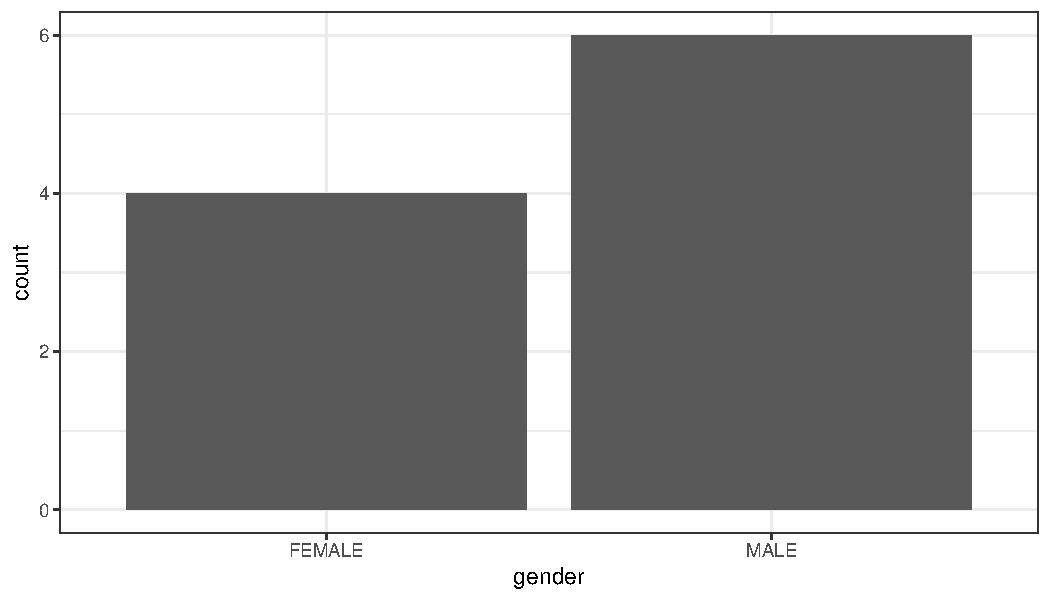
\includegraphics{Introductory-Statistics-with-R-tidyverse_files/figure-latex/unnamed-chunk-20-1} \end{center}

\hypertarget{using-r-functions-to-generate-multiple-frequency-tables}{%
\subsubsection{Using R Functions to Generate Multiple Frequency Tables}\label{using-r-functions-to-generate-multiple-frequency-tables}}

\begin{Shaded}
\begin{Highlighting}[]
\CommentTok{\# There are Multiple Categorical Variables in the dataset}
\CommentTok{\# Would be nice if we can generate frequency tables for all of them easily}
\CommentTok{\# Let\textquotesingle{}s create a list of  that are categorical}
\NormalTok{categorical.nomial.list \textless{}{-}}\StringTok{ }\KeywordTok{c}\NormalTok{(}\StringTok{\textquotesingle{}gender\textquotesingle{}}\NormalTok{, }\StringTok{\textquotesingle{}major\textquotesingle{}}\NormalTok{, }\StringTok{\textquotesingle{}games.any\textquotesingle{}}\NormalTok{, }\StringTok{\textquotesingle{}commute\textquotesingle{}}\NormalTok{, }\StringTok{\textquotesingle{}econ\textquotesingle{}}\NormalTok{)}
\end{Highlighting}
\end{Shaded}

\begin{Shaded}
\begin{Highlighting}[]
\CommentTok{\# Let\textquotesingle{}s Write a Function, not that we need to, but let\textquotesingle{}s do it}
\CommentTok{\# We can give the function any name, here: dplyr.freq.table}
\NormalTok{dplyr.freq.table \textless{}{-}}\StringTok{ }\ControlFlowTok{function}\NormalTok{(df, cate.var.str)\{}

    \CommentTok{\# A print Statement}
    \KeywordTok{print}\NormalTok{(}\KeywordTok{sprintf}\NormalTok{(}\StringTok{"From Dataset: \%s, Freq. Table for Variable: \%s"}\NormalTok{, }\KeywordTok{deparse}\NormalTok{(}\KeywordTok{substitute}\NormalTok{(df)), cate.var.str))}

    \CommentTok{\# Note below: !!sym(cate.var.str), because cate.var.str is string}
\NormalTok{    freq.table \textless{}{-}}\StringTok{ }\NormalTok{df }\OperatorTok{\%\textgreater{}\%}
\StringTok{        }\KeywordTok{group\_by}\NormalTok{(}\OperatorTok{!!}\KeywordTok{sym}\NormalTok{(cate.var.str)) }\OperatorTok{\%\textgreater{}\%}
\StringTok{        }\KeywordTok{summarise}\NormalTok{ (}\DataTypeTok{frequency.count =} \KeywordTok{n}\NormalTok{()) }\OperatorTok{\%\textgreater{}\%}
\StringTok{        }\KeywordTok{mutate}\NormalTok{(}\DataTypeTok{proportions =}\NormalTok{ frequency.count }\OperatorTok{/}\StringTok{ }\KeywordTok{sum}\NormalTok{(frequency.count))}

    \CommentTok{\# Function returns}
    \KeywordTok{return}\NormalTok{(freq.table)}
\NormalTok{\}}

\CommentTok{\# Let\textquotesingle{}s call test this function and generate our earlier table}
\KeywordTok{dplyr.freq.table}\NormalTok{(}\DataTypeTok{df =}\NormalTok{ df\_survey, }\DataTypeTok{cate.var.str =} \StringTok{\textquotesingle{}gender\textquotesingle{}}\NormalTok{)}
\end{Highlighting}
\end{Shaded}

\begin{verbatim}
## [1] "From Dataset: df_survey, Freq. Table for Variable: gender"
\end{verbatim}

\begin{Shaded}
\begin{Highlighting}[]
\CommentTok{\# Let\textquotesingle{}s Now Use our function to generate Multiple Frequency Tables}
\CommentTok{\# We will first use a explicit loop}
\ControlFlowTok{for}\NormalTok{ (ctr }\ControlFlowTok{in} \KeywordTok{seq\_along}\NormalTok{(categorical.nomial.list)) \{}
\NormalTok{    freq.table \textless{}{-}}\StringTok{ }\KeywordTok{dplyr.freq.table}\NormalTok{(}\DataTypeTok{df =}\NormalTok{ df\_survey, }\DataTypeTok{cate.var.str =}\NormalTok{ categorical.nomial.list[ctr])}
    \KeywordTok{print}\NormalTok{(freq.table)}
\NormalTok{\}}
\end{Highlighting}
\end{Shaded}

\begin{verbatim}
## [1] "From Dataset: df_survey, Freq. Table for Variable: gender"
## [1] "From Dataset: df_survey, Freq. Table for Variable: major"
## [1] "From Dataset: df_survey, Freq. Table for Variable: games.any"
## [1] "From Dataset: df_survey, Freq. Table for Variable: commute"
## [1] "From Dataset: df_survey, Freq. Table for Variable: econ"
\end{verbatim}

Using Lapply to Generate Multiple Frequency Tables with a Single Line:

\begin{Shaded}
\begin{Highlighting}[]
\CommentTok{\# We will now use lapply, the single line loop tool in R}
\CommentTok{\# Below, we are plugging each element of the list one by one into the function}
\CommentTok{\# dplyr.freq.table, the first argument of the function is the dataset name}
\CommentTok{\# which is fixed as df = df\_survey}
\KeywordTok{lapply}\NormalTok{(categorical.nomial.list,}
\NormalTok{       dplyr.freq.table,}
       \DataTypeTok{df =}\NormalTok{ df\_survey)}
\end{Highlighting}
\end{Shaded}

\begin{verbatim}
## [1] "From Dataset: df_survey, Freq. Table for Variable: gender"
## [1] "From Dataset: df_survey, Freq. Table for Variable: major"
## [1] "From Dataset: df_survey, Freq. Table for Variable: games.any"
## [1] "From Dataset: df_survey, Freq. Table for Variable: commute"
## [1] "From Dataset: df_survey, Freq. Table for Variable: econ"
\end{verbatim}

\begin{verbatim}
## [[1]]
## 
## [[2]]
## 
## [[3]]
## 
## [[4]]
## 
## [[5]]
\end{verbatim}

\hypertarget{continuousquantitative}{%
\subsection{Continuous/Quantitative}\label{continuousquantitative}}

Graphically, we can show a continuous variable using a histogram. This could be test scores, temperatures, years in Houston, etc. This involves first creating a categorical/discrete variable based on the continuous variable. Since the underlying continuous variable is ordered (low to high temperature unless major which is not ordered), the categorical/discrete variable we generate is an ordered categorical variable (majors could be called unordered categorical variable).

\hypertarget{histogram-with-lapply}{%
\subsubsection{Histogram with Lapply}\label{histogram-with-lapply}}

To generate the histogram, we:
1. Make sure that all observations belongs to one category
+ no observations belonging to no categories
+ each observation only belongs to one category
2. Each category is equidistance along the continuous variable's original scale.
3. Then we create a bar graph where each bar is a category, and the height of the bar represents the number of observations within that category.

\begin{Shaded}
\begin{Highlighting}[]
\CommentTok{\# We will write a histogram function}
\NormalTok{ggplot.histogram \textless{}{-}}\StringTok{ }\ControlFlowTok{function}\NormalTok{(df, cts.var.str)\{}

    \CommentTok{\# Figure Size}
    \KeywordTok{options}\NormalTok{(}\DataTypeTok{repr.plot.width =} \DecValTok{4}\NormalTok{, }\DataTypeTok{repr.plot.height =} \DecValTok{3}\NormalTok{)}

    \CommentTok{\# Figure Title}
\NormalTok{    title \textless{}{-}}\StringTok{ }\KeywordTok{sprintf}\NormalTok{(}\StringTok{"Histogram for \%s in \%s"}\NormalTok{, cts.var.str, }\KeywordTok{deparse}\NormalTok{(}\KeywordTok{substitute}\NormalTok{(df)))}

    \CommentTok{\# We have in our 10 student survey only 10 observations}
    \CommentTok{\# We can still generate a histogram for our continuous variables}
    \CommentTok{\# Will only use three bins}
\NormalTok{    histogram}\FloatTok{.3}\NormalTok{bins \textless{}{-}}\StringTok{ }\KeywordTok{ggplot}\NormalTok{(df\_survey, }\KeywordTok{aes}\NormalTok{(}\DataTypeTok{x=}\OperatorTok{!!}\KeywordTok{sym}\NormalTok{(cts.var.str))) }\OperatorTok{+}
\StringTok{      }\KeywordTok{geom\_histogram}\NormalTok{(}\DataTypeTok{bins=}\DecValTok{3}\NormalTok{) }\OperatorTok{+}
\StringTok{      }\KeywordTok{labs}\NormalTok{(}\DataTypeTok{title =} \KeywordTok{paste0}\NormalTok{(title),}
           \DataTypeTok{caption =} \StringTok{\textquotesingle{}In Class Survey of 10 Students}\CharTok{\textbackslash{}n}\StringTok{3 bins\textquotesingle{}}\NormalTok{) }\OperatorTok{+}
\StringTok{      }\KeywordTok{theme\_bw}\NormalTok{()}

    \CommentTok{\# obtain the data in the plot}
\NormalTok{    plot\_data \textless{}{-}}\StringTok{ }\KeywordTok{ggplot\_build}\NormalTok{(histogram}\FloatTok{.3}\NormalTok{bins)}
    \CommentTok{\# the dataframe below contains all the information for the histogram}
    \CommentTok{\# bins and number of observations in each bins}
\NormalTok{    plot\_dataframe \textless{}{-}}\StringTok{ }\NormalTok{plot\_data}\OperatorTok{$}\NormalTok{data[[}\DecValTok{1}\NormalTok{]]}

    \CommentTok{\# return outputs}
    \KeywordTok{return}\NormalTok{(}\KeywordTok{list}\NormalTok{(}\DataTypeTok{gghist=}\NormalTok{histogram}\FloatTok{.3}\NormalTok{bins, }\DataTypeTok{hist.df=}\NormalTok{plot\_dataframe))}
\NormalTok{\}}
\end{Highlighting}
\end{Shaded}

\begin{Shaded}
\begin{Highlighting}[]
\CommentTok{\# Now the list of continuous Variables and calling the function with lapply}
\NormalTok{cts.list \textless{}{-}}\StringTok{ }\KeywordTok{c}\NormalTok{(}\StringTok{\textquotesingle{}years.in.houston\textquotesingle{}}\NormalTok{, }\StringTok{\textquotesingle{}games.attended\textquotesingle{}}\NormalTok{)}

\CommentTok{\# lapply}
\NormalTok{results \textless{}{-}}\StringTok{ }\KeywordTok{lapply}\NormalTok{(cts.list,}
\NormalTok{       ggplot.histogram,}
       \DataTypeTok{df =}\NormalTok{ df\_survey)}

\CommentTok{\# Show results}
\ControlFlowTok{for}\NormalTok{ (ctr }\ControlFlowTok{in} \KeywordTok{seq\_along}\NormalTok{(cts.list))\{}
    \KeywordTok{print}\NormalTok{(results[ctr])}
\NormalTok{\}}
\end{Highlighting}
\end{Shaded}

\begin{verbatim}
## [[1]]
## [[1]]$gghist
\end{verbatim}

\begin{center}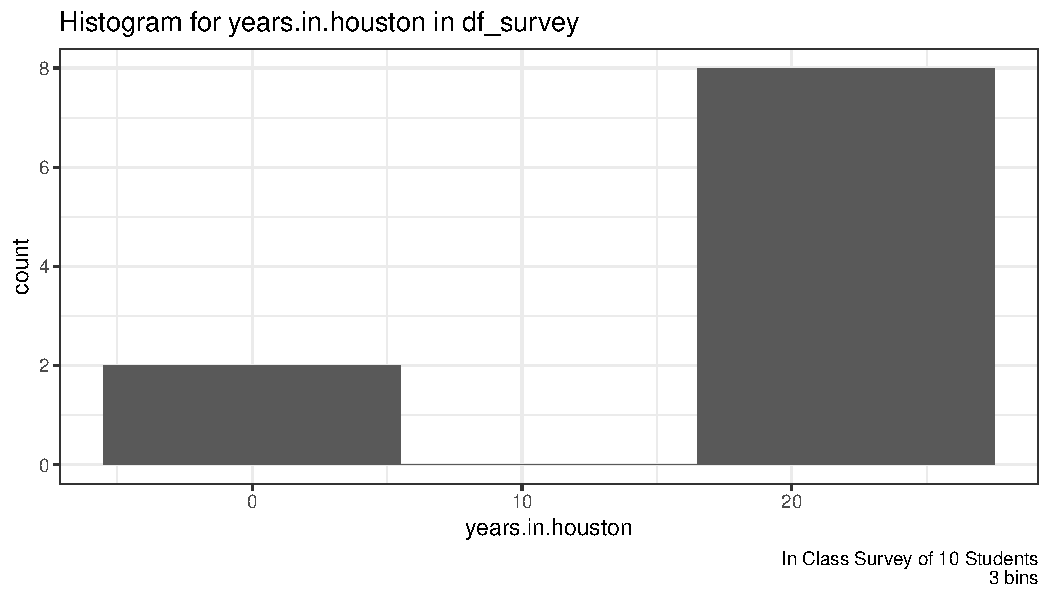
\includegraphics{Introductory-Statistics-with-R-tidyverse_files/figure-latex/unnamed-chunk-26-1} \end{center}

\begin{verbatim}
## 
## [[1]]$hist.df
##   y count  x xmin xmax    density ncount ndensity flipped_aes PANEL group ymin ymax colour   fill size linetype alpha
## 1 2     2  0 -5.5  5.5 0.01818182   0.25     0.25       FALSE     1    -1    0    2     NA grey35  0.5        1    NA
## 2 0     0 11  5.5 16.5 0.00000000   0.00     0.00       FALSE     1    -1    0    0     NA grey35  0.5        1    NA
## 3 8     8 22 16.5 27.5 0.07272727   1.00     1.00       FALSE     1    -1    0    8     NA grey35  0.5        1    NA
## 
## 
## [[1]]
## [[1]]$gghist
\end{verbatim}

\begin{center}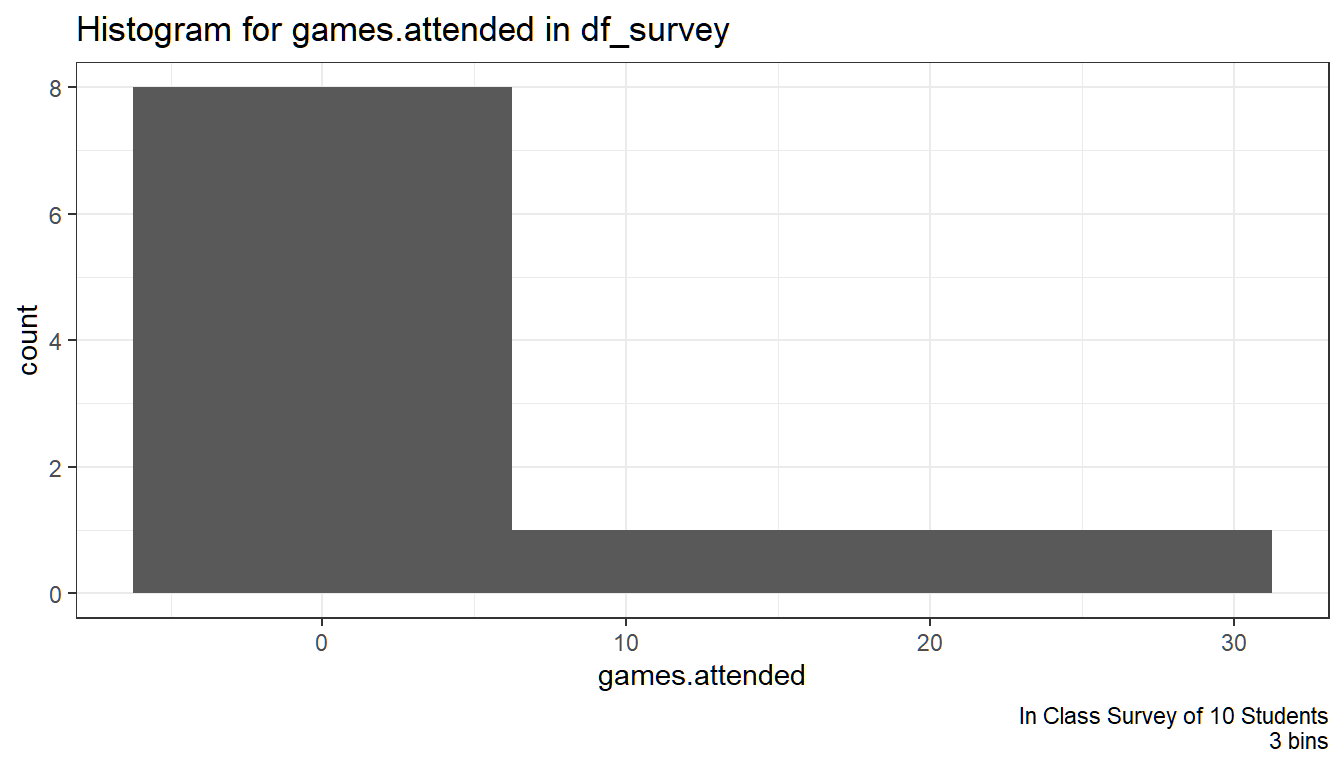
\includegraphics{Introductory-Statistics-with-R-tidyverse_files/figure-latex/unnamed-chunk-26-2} \end{center}

\begin{verbatim}
## 
## [[1]]$hist.df
##   y count    x  xmin  xmax density ncount ndensity flipped_aes PANEL group ymin ymax colour   fill size linetype alpha
## 1 8     8  0.0 -6.25  6.25   0.064  1.000    1.000       FALSE     1    -1    0    8     NA grey35  0.5        1    NA
## 2 1     1 12.5  6.25 18.75   0.008  0.125    0.125       FALSE     1    -1    0    1     NA grey35  0.5        1    NA
## 3 1     1 25.0 18.75 31.25   0.008  0.125    0.125       FALSE     1    -1    0    1     NA grey35  0.5        1    NA
\end{verbatim}

\hypertarget{multiple-variables-graphs-and-tables}{%
\section{Multiple Variables Graphs and Tables}\label{multiple-variables-graphs-and-tables}}

\begin{quote}
Go back to \href{http://fanwangecon.github.io/}{fan}'s \href{https://fanwangecon.github.io/REconTools/}{REconTools} Package, \href{https://fanwangecon.github.io/R4Econ/}{R Code Examples} Repository (\href{https://fanwangecon.github.io/R4Econ/bookdown}{bookdown site}), or \href{https://fanwangecon.github.io/Stat4Econ/}{Intro Stats with R} Repository (\href{https://fanwangecon.github.io/Stat4Econ/bookdown}{bookdown site}).
\end{quote}

\begin{Shaded}
\begin{Highlighting}[]
\CommentTok{\# For Data Manipulations}
\KeywordTok{library}\NormalTok{(tidyverse)}
\CommentTok{\# For Additional table output}
\CommentTok{\# install.packages("knitr")}
\KeywordTok{library}\NormalTok{(knitr)}
\end{Highlighting}
\end{Shaded}

Let's load in the dataset we created from the \href{https://fanwangecon.github.io/Stat4Econ/survey/htmlpdfr/classsurvey.html}{in-class survey}.

\begin{Shaded}
\begin{Highlighting}[]
\CommentTok{\# Load the dataset using readr\textquotesingle{}s read\_csv}
\NormalTok{df\_survey \textless{}{-}}\StringTok{ }\KeywordTok{read\_csv}\NormalTok{(}\StringTok{\textquotesingle{}data/classsurvey.csv\textquotesingle{}}\NormalTok{)}
\end{Highlighting}
\end{Shaded}

\begin{Shaded}
\begin{Highlighting}[]
\CommentTok{\# We have several factor variables, we can set them as factor one by one}
\NormalTok{df\_survey[[}\StringTok{\textquotesingle{}gender\textquotesingle{}}\NormalTok{]] \textless{}{-}}\StringTok{ }\KeywordTok{as.factor}\NormalTok{(df\_survey[[}\StringTok{\textquotesingle{}gender\textquotesingle{}}\NormalTok{]])}
\CommentTok{\# But that is a little cumbersome, we can using lapply, a core function in r to do this for all factors}
\NormalTok{factor\_col\_names \textless{}{-}}\StringTok{ }\KeywordTok{c}\NormalTok{(}\StringTok{\textquotesingle{}gender\textquotesingle{}}\NormalTok{, }\StringTok{\textquotesingle{}major\textquotesingle{}}\NormalTok{, }\StringTok{\textquotesingle{}commute\textquotesingle{}}\NormalTok{, }\StringTok{\textquotesingle{}games.any\textquotesingle{}}\NormalTok{, }\StringTok{\textquotesingle{}econ\textquotesingle{}}\NormalTok{)}
\NormalTok{df\_survey[factor\_col\_names] \textless{}{-}}\StringTok{ }\KeywordTok{lapply}\NormalTok{(df\_survey[factor\_col\_names], as.factor)}
\CommentTok{\# Check Variable Types}
\KeywordTok{str}\NormalTok{(df\_survey)}
\end{Highlighting}
\end{Shaded}

\begin{verbatim}
## tibble [10 x 10] (S3: spec_tbl_df/tbl_df/tbl/data.frame)
##  $ ID              : num [1:10] 1 2 3 4 5 6 7 8 9 10
##  $ ROW             : num [1:10] 3 4 4 4 2 1 2 3 3 4
##  $ COL             : num [1:10] 1 2 10 1 6 7 6 6 3 13
##  $ gender          : Factor w/ 2 levels "FEMALE","MALE": 2 1 2 2 1 2 2 2 1 1
##  $ years.in.houston: num [1:10] 21 21 22 22 20 3 25 20 5 20
##  $ major           : Factor w/ 5 levels "CONSUMERSCIENCE",..: 2 3 2 2 2 5 2 1 4 2
##  $ commute         : Factor w/ 1 level "YES": 1 1 1 1 1 1 1 1 1 1
##  $ games.attended  : num [1:10] 0 2 0 14 0 0 25 2 0 0
##  $ games.any       : Factor w/ 2 levels "Has.Attended",..: 2 1 2 1 2 2 1 1 2 2
##  $ econ            : Factor w/ 2 levels "ECON","Not.Econ": 1 2 1 1 1 2 1 2 2 1
##  - attr(*, "spec")=
##   .. cols(
##   ..   ID = col_double(),
##   ..   ROW = col_double(),
##   ..   COL = col_double(),
##   ..   gender = col_character(),
##   ..   years.in.houston = col_double(),
##   ..   major = col_character(),
##   ..   commute = col_character(),
##   ..   games.attended = col_double(),
##   ..   games.any = col_character(),
##   ..   econ = col_character()
##   .. )
\end{verbatim}

\hypertarget{two-continuous-variables}{%
\subsection{Two Continuous Variables}\label{two-continuous-variables}}

With two continuous/quantitative variables, we can generate a scatter plot. Crucially, each point of the scatter plot represents one individual, the location of that point indicates the x and y values of that individual. The x and y values could be the individual's test score and hours studied for example.

\begin{Shaded}
\begin{Highlighting}[]
\CommentTok{\# We can draw a scatter plot for two continuous variables}
\CommentTok{\# Control Graph Size}
\KeywordTok{options}\NormalTok{(}\DataTypeTok{repr.plot.width =} \DecValTok{4}\NormalTok{, }\DataTypeTok{repr.plot.height =} \DecValTok{4}\NormalTok{)}
\CommentTok{\# Draw Scatter Plot}
\CommentTok{\# 1. specify x and y}
\CommentTok{\# 2. label each individual by their ID, add letter I in front of value}
\CommentTok{\# 3. add in trend line}
\NormalTok{scatter \textless{}{-}}\StringTok{ }\KeywordTok{ggplot}\NormalTok{(df\_survey, }\KeywordTok{aes}\NormalTok{(}\DataTypeTok{x=}\NormalTok{games.attended, }\DataTypeTok{y=}\NormalTok{years.in.houston)) }\OperatorTok{+}
\StringTok{      }\KeywordTok{geom\_point}\NormalTok{(}\DataTypeTok{size=}\DecValTok{1}\NormalTok{) }\OperatorTok{+}
\StringTok{      }\KeywordTok{geom\_text}\NormalTok{(}\KeywordTok{aes}\NormalTok{(}\DataTypeTok{label=}\KeywordTok{paste0}\NormalTok{(}\StringTok{\textquotesingle{}I\textquotesingle{}}\NormalTok{, ID)), }\DataTypeTok{size=}\DecValTok{3}\NormalTok{, }\DataTypeTok{hjust=}\OperatorTok{{-}}\NormalTok{.}\DecValTok{2}\NormalTok{, }\DataTypeTok{vjust=}\OperatorTok{{-}}\NormalTok{.}\DecValTok{2}\NormalTok{) }\OperatorTok{+}
\StringTok{      }\KeywordTok{geom\_smooth}\NormalTok{(}\DataTypeTok{method=}\NormalTok{lm) }\OperatorTok{+}\StringTok{ }\CommentTok{\# Trend line}
\StringTok{      }\KeywordTok{labs}\NormalTok{(}\DataTypeTok{title =} \KeywordTok{paste0}\NormalTok{(}\StringTok{\textquotesingle{}Scatter Plot of Two Continuous/Quantitative Variables\textquotesingle{}}
\NormalTok{                          ,}\StringTok{\textquotesingle{}}\CharTok{\textbackslash{}n}\StringTok{In Class Survey of 10 Students\textquotesingle{}}\NormalTok{),}
           \DataTypeTok{x =} \StringTok{\textquotesingle{}Games Attended at the University\textquotesingle{}}\NormalTok{,}
           \DataTypeTok{y =} \StringTok{\textquotesingle{}Years Spent in the City of Houston\textquotesingle{}}\NormalTok{,}
           \DataTypeTok{caption =} \StringTok{\textquotesingle{}In Class Survey\textquotesingle{}}\NormalTok{) }\OperatorTok{+}
\StringTok{      }\KeywordTok{theme\_bw}\NormalTok{()}
\KeywordTok{print}\NormalTok{(scatter)}
\end{Highlighting}
\end{Shaded}

\begin{center}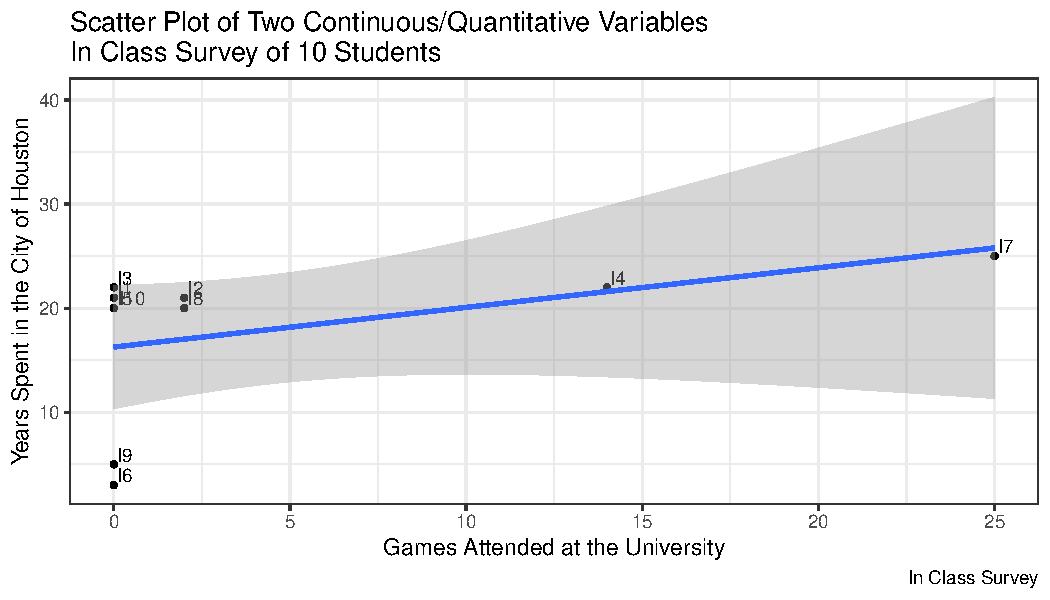
\includegraphics{Introductory-Statistics-with-R-tidyverse_files/figure-latex/unnamed-chunk-31-1} \end{center}

\hypertarget{two-categorical-variables}{%
\subsection{Two Categorical Variables}\label{two-categorical-variables}}

With two discrete/categorical variables, we can generate two-way frequency tables. This is very similar to what we did for one discrete variable, except now we have columns and rows, representing the categories of the two variables. The two variables could be gender and majors, we would write in each table cell the number of students who are male and econ majors, male and bio majors in for example the first column, and repeat this for girls in the second column.

\begin{Shaded}
\begin{Highlighting}[]
\CommentTok{\# We can tabulate Frequencies based on two categorical variables}
\NormalTok{df\_survey }\OperatorTok{\%\textgreater{}\%}
\StringTok{  }\KeywordTok{group\_by}\NormalTok{(gender, econ) }\OperatorTok{\%\textgreater{}\%}
\StringTok{  }\KeywordTok{summarize}\NormalTok{(}\DataTypeTok{freq =} \KeywordTok{n}\NormalTok{()) }\OperatorTok{\%\textgreater{}\%}
\StringTok{  }\KeywordTok{spread}\NormalTok{(gender, freq)}
\end{Highlighting}
\end{Shaded}

\begin{Shaded}
\begin{Highlighting}[]
\CommentTok{\# We can show the fraction of individuals in each of the four groups}
\NormalTok{df\_survey }\OperatorTok{\%\textgreater{}\%}
\StringTok{  }\KeywordTok{group\_by}\NormalTok{(}\KeywordTok{interaction}\NormalTok{(gender, econ)) }\OperatorTok{\%\textgreater{}\%}
\StringTok{  }\KeywordTok{summarise}\NormalTok{(}\DataTypeTok{freq =} \KeywordTok{n}\NormalTok{()) }\OperatorTok{\%\textgreater{}\%}
\StringTok{  }\KeywordTok{mutate}\NormalTok{(}\DataTypeTok{fraction =}\NormalTok{ freq }\OperatorTok{/}\StringTok{ }\KeywordTok{sum}\NormalTok{(freq))}
\end{Highlighting}
\end{Shaded}

\begin{Shaded}
\begin{Highlighting}[]
\CommentTok{\# We can create stacked bar charts as well with the same data}
\CommentTok{\# graph size}
\KeywordTok{options}\NormalTok{(}\DataTypeTok{repr.plot.width =} \DecValTok{3}\NormalTok{, }\DataTypeTok{repr.plot.height =} \DecValTok{2}\NormalTok{)}
\CommentTok{\# Graph}
\NormalTok{stacked.bar.plot \textless{}{-}}\StringTok{ }\KeywordTok{ggplot}\NormalTok{(df\_survey) }\OperatorTok{+}
\StringTok{    }\KeywordTok{geom\_bar}\NormalTok{(}\KeywordTok{aes}\NormalTok{(}\DataTypeTok{x=}\NormalTok{gender, }\DataTypeTok{fill=}\NormalTok{econ)) }\OperatorTok{+}
\StringTok{    }\KeywordTok{theme\_bw}\NormalTok{()}
\KeywordTok{print}\NormalTok{(stacked.bar.plot)}
\end{Highlighting}
\end{Shaded}

\begin{center}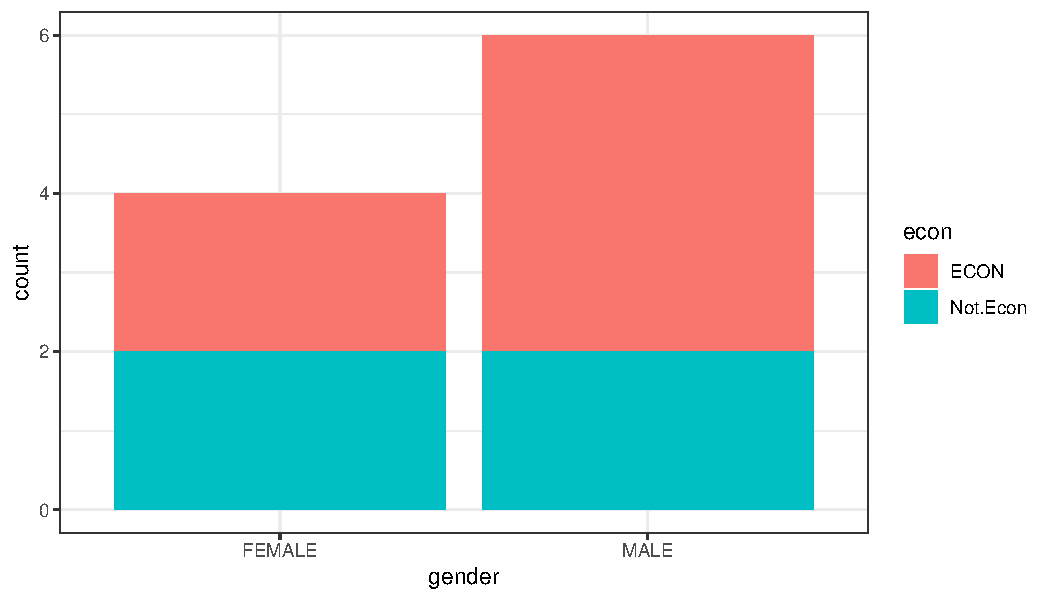
\includegraphics{Introductory-Statistics-with-R-tidyverse_files/figure-latex/unnamed-chunk-34-1} \end{center}

\hypertarget{continuous-and-categorical-variable}{%
\subsection{Continuous and Categorical Variable}\label{continuous-and-categorical-variable}}

\hypertarget{average-across-groups}{%
\subsubsection{Average Across Groups}\label{average-across-groups}}

We can look at the average game attendance by female and male students in our sample, using a bar plot, where the height of the bars now represent the average of the \emph{games.attended} variable for each group.

\begin{Shaded}
\begin{Highlighting}[]
\CommentTok{\# We can first find the group averages}
\NormalTok{df\_gender\_avg\_games \textless{}{-}}\StringTok{ }\NormalTok{df\_survey }\OperatorTok{\%\textgreater{}\%}
\StringTok{                        }\KeywordTok{group\_by}\NormalTok{(gender) }\OperatorTok{\%\textgreater{}\%}
\StringTok{                        }\KeywordTok{summarise}\NormalTok{ (}\DataTypeTok{avg.games.attended =} \KeywordTok{mean}\NormalTok{(games.attended))}
\NormalTok{df\_gender\_avg\_games}
\end{Highlighting}
\end{Shaded}

\begin{Shaded}
\begin{Highlighting}[]
\CommentTok{\# We can graph based on df\_gender\_avg\_games}
\CommentTok{\# Sizing the Figure Here}
\KeywordTok{options}\NormalTok{(}\DataTypeTok{repr.plot.width =} \DecValTok{2}\NormalTok{, }\DataTypeTok{repr.plot.height =} \DecValTok{2}\NormalTok{)}
\CommentTok{\# Plot, stat = identity means to plot the value in avg.games.attended for each gender}
\NormalTok{group.means \textless{}{-}}\StringTok{ }\KeywordTok{ggplot}\NormalTok{(df\_gender\_avg\_games) }\OperatorTok{+}
\StringTok{    }\KeywordTok{geom\_bar}\NormalTok{(}\KeywordTok{aes}\NormalTok{(}\DataTypeTok{x=}\NormalTok{gender, }\DataTypeTok{y=}\NormalTok{avg.games.attended), }\DataTypeTok{stat =} \StringTok{\textquotesingle{}identity\textquotesingle{}}\NormalTok{) }\OperatorTok{+}
\StringTok{    }\KeywordTok{theme\_bw}\NormalTok{()}
\KeywordTok{print}\NormalTok{(group.means)}
\end{Highlighting}
\end{Shaded}

\begin{center}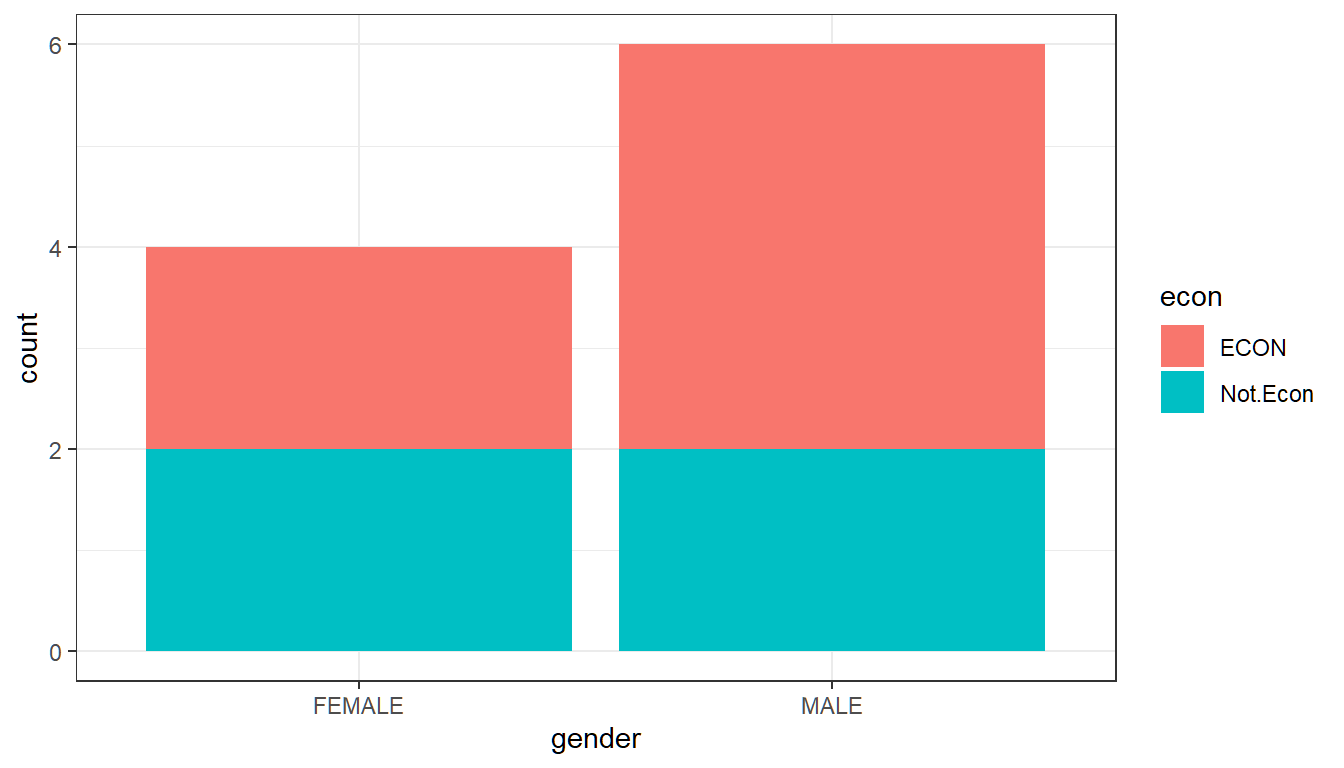
\includegraphics{Introductory-Statistics-with-R-tidyverse_files/figure-latex/unnamed-chunk-36-1} \end{center}

\begin{Shaded}
\begin{Highlighting}[]
\CommentTok{\# But it is a little cumbersome to do this in two steps, we can do it in one step}
\CommentTok{\# Sizing the Figure Here}
\KeywordTok{options}\NormalTok{(}\DataTypeTok{repr.plot.width =} \DecValTok{2}\NormalTok{, }\DataTypeTok{repr.plot.height =} \DecValTok{2}\NormalTok{)}
\CommentTok{\# Plot directly from df\_survey, summary over x for y}
\CommentTok{\# The result looks the same}
\NormalTok{group.means.joint \textless{}{-}}\StringTok{ }\KeywordTok{ggplot}\NormalTok{(df\_survey) }\OperatorTok{+}
\StringTok{    }\KeywordTok{geom\_bar}\NormalTok{(}\KeywordTok{aes}\NormalTok{(}\DataTypeTok{x=}\NormalTok{gender, }\DataTypeTok{y=}\NormalTok{games.attended), }\DataTypeTok{stat =} \StringTok{"summary"}\NormalTok{, }\DataTypeTok{fun.y =} \StringTok{"mean"}\NormalTok{) }\OperatorTok{+}
\StringTok{    }\KeywordTok{theme\_bw}\NormalTok{()}
\KeywordTok{print}\NormalTok{(group.means.joint)}
\end{Highlighting}
\end{Shaded}

\begin{center}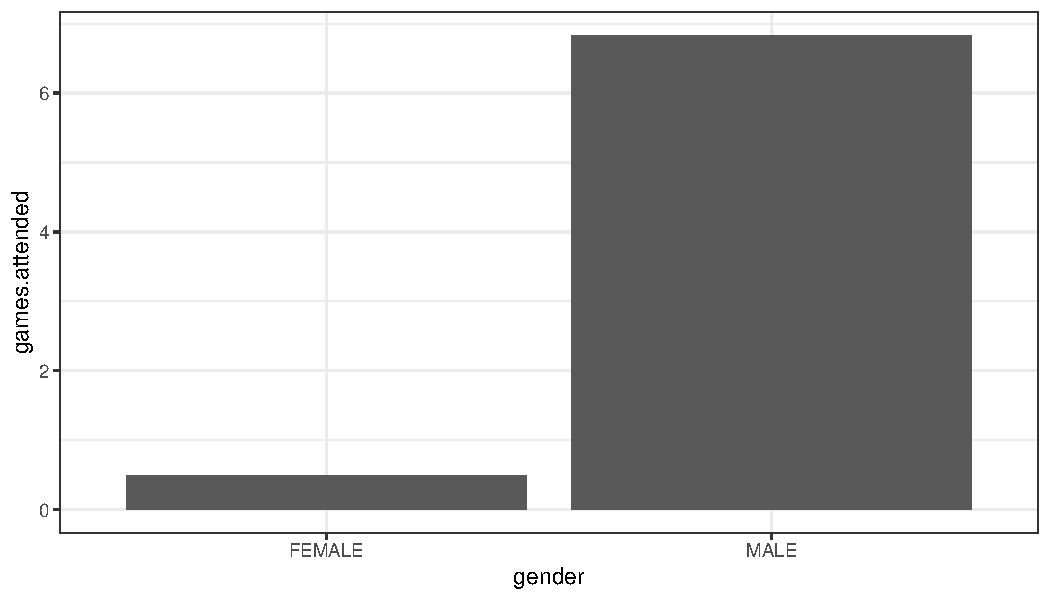
\includegraphics{Introductory-Statistics-with-R-tidyverse_files/figure-latex/unnamed-chunk-37-1} \end{center}

\hypertarget{average-across-two-groups-gender-and-majors}{%
\subsubsection{Average Across Two Groups: Gender and Majors}\label{average-across-two-groups-gender-and-majors}}

What is the average game attendance for male and female, econ and non-econ majors? We have 2 female econ majors, 2 female non-econ majors, 4 male econ majors and 2 male non-econ majors, and their average game attendances are: 0, 1, 9.75 and 1 games.

\begin{Shaded}
\begin{Highlighting}[]
\CommentTok{\# We can calculate the statistics as a table, and also show obs in each group}
\NormalTok{df\_survey }\OperatorTok{\%\textgreater{}\%}
\StringTok{    }\KeywordTok{group\_by}\NormalTok{(gender, econ ) }\OperatorTok{\%\textgreater{}\%}
\StringTok{    }\KeywordTok{summarise}\NormalTok{ (}\DataTypeTok{avg.games.attended =} \KeywordTok{mean}\NormalTok{(games.attended), }\DataTypeTok{N.count =} \KeywordTok{n}\NormalTok{())}
\end{Highlighting}
\end{Shaded}

\begin{Shaded}
\begin{Highlighting}[]
\CommentTok{\# Let\textquotesingle{}s Show these Visually}
\KeywordTok{options}\NormalTok{(}\DataTypeTok{repr.plot.width =} \DecValTok{4}\NormalTok{, }\DataTypeTok{repr.plot.height =} \DecValTok{2}\NormalTok{)}
\CommentTok{\# Plot directly from df\_survey}
\CommentTok{\# Using fill for econ, this means econ or not will fill up with different colors}
\CommentTok{\# Still caculate average}
\CommentTok{\# Postion "dodge" means that econ and non{-}econ wil be shown next to each other}
\CommentTok{\# By default position is to stack different fill groups on top of each other.}
\NormalTok{two.group.means \textless{}{-}}\StringTok{ }\KeywordTok{ggplot}\NormalTok{(df\_survey) }\OperatorTok{+}
\StringTok{    }\KeywordTok{geom\_bar}\NormalTok{(}\KeywordTok{aes}\NormalTok{(}\DataTypeTok{x=}\NormalTok{gender, }\DataTypeTok{y=}\NormalTok{games.attended, }\DataTypeTok{fill=}\NormalTok{econ),}
             \DataTypeTok{stat =} \StringTok{"summary"}\NormalTok{, }\DataTypeTok{fun.y =} \StringTok{"mean"}\NormalTok{, }\DataTypeTok{position =} \StringTok{"dodge"}\NormalTok{) }\OperatorTok{+}
\StringTok{    }\KeywordTok{theme\_bw}\NormalTok{()}
\KeywordTok{print}\NormalTok{(two.group.means)}
\end{Highlighting}
\end{Shaded}

\begin{center}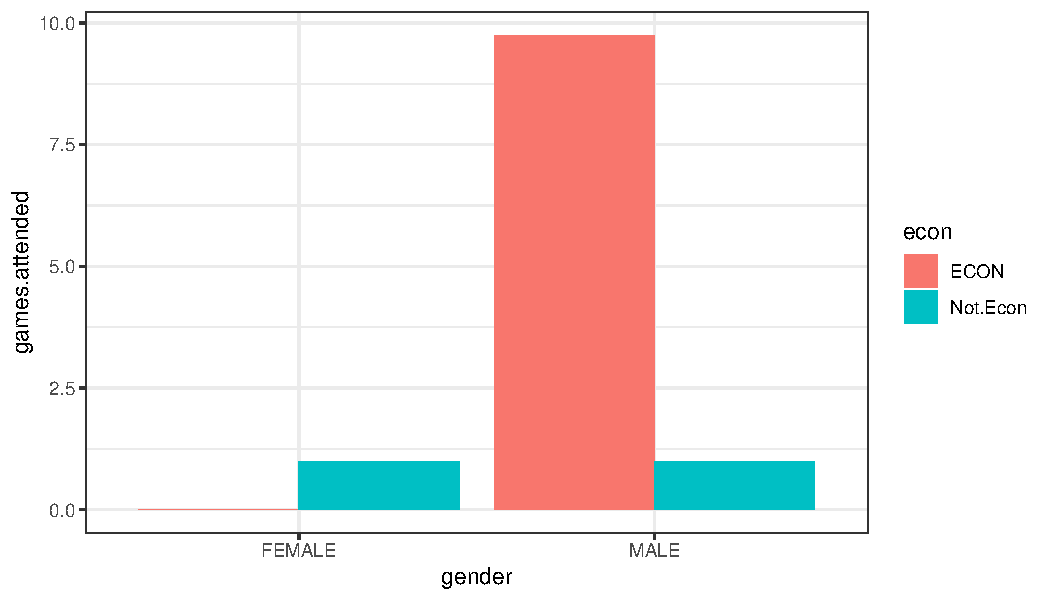
\includegraphics{Introductory-Statistics-with-R-tidyverse_files/figure-latex/unnamed-chunk-39-1} \end{center}

\hypertarget{summarizing-data}{%
\chapter{Summarizing Data}\label{summarizing-data}}

\hypertarget{mean-and-standard-deviation}{%
\section{Mean and Standard Deviation}\label{mean-and-standard-deviation}}

\begin{quote}
Go back to \href{http://fanwangecon.github.io/}{fan}'s \href{https://fanwangecon.github.io/REconTools/}{REconTools} Package, \href{https://fanwangecon.github.io/R4Econ/}{R Code Examples} Repository (\href{https://fanwangecon.github.io/R4Econ/bookdown}{bookdown site}), or \href{https://fanwangecon.github.io/Stat4Econ/}{Intro Stats with R} Repository (\href{https://fanwangecon.github.io/Stat4Econ/bookdown}{bookdown site}).
\end{quote}

\hypertarget{temperature-across-locations-over-time}{%
\subsection{Temperature Across Locations over Time}\label{temperature-across-locations-over-time}}

Why do we need the standard deviation? We will demonstrate its usefulness by studying temperature dataset. This dataset covers a variety of cities in the United States across all States and Territories. For each city, we have the average temperature in each month. The unit of observation is at the city/month level. We have variables for the state, the city, the month and the average temperature.

\textbf{The dataset, \emph{TempCitiesUSA.csv}, can be downloaded \href{https://github.com/FanWangEcon/Stat4Econ/tree/master/data/TempCitiesUSA.csv}{here}.}

\begin{Shaded}
\begin{Highlighting}[]
\CommentTok{\# Load in Data Tools}
\CommentTok{\# For Reading/Loading Data}
\KeywordTok{library}\NormalTok{(tidyverse)}
\CommentTok{\# Load in Data}
\NormalTok{df\_temp \textless{}{-}}\StringTok{ }\KeywordTok{read\_csv}\NormalTok{(}\StringTok{\textquotesingle{}data/TempCitiesUSA.csv\textquotesingle{}}\NormalTok{)}
\end{Highlighting}
\end{Shaded}

\textbf{Listing Unique Levels for Categorical Variables in the Dataset}

We can see that the state and city variables are string variables. We can show unique states and cities by months. In the program below, I append the number of observations for each category.

From the tables below, we can see that each city has 12 observations (for the 12 months), and each state has multiple cities.

\begin{Shaded}
\begin{Highlighting}[]
\CommentTok{\# A function that shows Unique Values for Categorical Variables in a Table format}
\NormalTok{show.unique.values \textless{}{-}}\StringTok{ }\ControlFlowTok{function}\NormalTok{(df, cate.var.str, }\DataTypeTok{lvl\_str\_max\_len=}\DecValTok{15}\NormalTok{)\{}

    \CommentTok{\# Unique Categories}
\NormalTok{    unique.cates \textless{}{-}}\StringTok{ }\NormalTok{df }\OperatorTok{\%\textgreater{}\%}
\StringTok{        }\KeywordTok{group\_by}\NormalTok{(}\OperatorTok{!!}\KeywordTok{sym}\NormalTok{(cate.var.str)) }\OperatorTok{\%\textgreater{}\%}
\StringTok{        }\KeywordTok{summarise}\NormalTok{(}\DataTypeTok{freq =} \KeywordTok{n}\NormalTok{()) }\OperatorTok{\%\textgreater{}\%}
\StringTok{        }\KeywordTok{mutate}\NormalTok{(}\DataTypeTok{distinct\_N =} \KeywordTok{paste0}\NormalTok{(}\OperatorTok{!!}\KeywordTok{sym}\NormalTok{(cate.var.str), }\StringTok{\textquotesingle{} (n=\textquotesingle{}}\NormalTok{, freq, }\StringTok{\textquotesingle{})\textquotesingle{}}\NormalTok{)) }\OperatorTok{\%\textgreater{}\%}
\StringTok{        }\KeywordTok{select}\NormalTok{(distinct\_N)}

    \CommentTok{\# At most 10 columns}
\NormalTok{    unique.count \textless{}{-}}\StringTok{ }\KeywordTok{dim}\NormalTok{(unique.cates)[}\DecValTok{1}\NormalTok{]}
\NormalTok{    col.count \textless{}{-}}\StringTok{ }\KeywordTok{min}\NormalTok{(}\KeywordTok{ceiling}\NormalTok{(}\KeywordTok{sqrt}\NormalTok{(unique.count)), }\DecValTok{8}\NormalTok{)}
\NormalTok{    row.count \textless{}{-}}\StringTok{ }\KeywordTok{ceiling}\NormalTok{(unique.count}\OperatorTok{/}\NormalTok{col.count)}

    \CommentTok{\# Generate Table to Fill in}
\NormalTok{    expand.length =}\StringTok{ }\NormalTok{row.count}\OperatorTok{*}\NormalTok{col.count}
\NormalTok{    unique.cates.expand \textless{}{-}}\StringTok{ }\KeywordTok{vector}\NormalTok{(}\DataTypeTok{mode =} \StringTok{"character"}\NormalTok{, }\DataTypeTok{length =}\NormalTok{ expand.length)}

    \CommentTok{\# Unique Categories and Counts}
\NormalTok{    unique.cates.shorter \textless{}{-}}\StringTok{ }\KeywordTok{substring}\NormalTok{(}\KeywordTok{t}\NormalTok{(unique.cates), }\DataTypeTok{first =} \DecValTok{1}\NormalTok{, }\DataTypeTok{last =}\NormalTok{ lvl\_str\_max\_len)}
\NormalTok{    unique.cates.expand[}\DecValTok{0}\OperatorTok{:}\NormalTok{unique.count] \textless{}{-}}\StringTok{ }\NormalTok{unique.cates.shorter}

    \CommentTok{\# Reshape}
    \KeywordTok{dim}\NormalTok{(unique.cates.expand) \textless{}{-}}\StringTok{ }\KeywordTok{c}\NormalTok{(row.count, col.count)}

    \CommentTok{\# Show}
\NormalTok{    title \textless{}{-}}\StringTok{ }\KeywordTok{sprintf}\NormalTok{(}\StringTok{"From Dataset: \%s, \%d unique Levels for: \%s"}\NormalTok{,}
                     \KeywordTok{deparse}\NormalTok{(}\KeywordTok{substitute}\NormalTok{(df)), unique.count, cate.var.str)}
    \KeywordTok{return}\NormalTok{(}\KeywordTok{list}\NormalTok{(}\DataTypeTok{title=}\NormalTok{title,}
           \DataTypeTok{levels=}\NormalTok{unique.cates.expand))}
\NormalTok{\}}
\end{Highlighting}
\end{Shaded}

\begin{Shaded}
\begin{Highlighting}[]
\CommentTok{\# List of categorical Variables}
\NormalTok{cate.vars.list \textless{}{-}}\StringTok{ }\KeywordTok{c}\NormalTok{(}\StringTok{\textquotesingle{}month\textquotesingle{}}\NormalTok{, }\StringTok{\textquotesingle{}state\textquotesingle{}}\NormalTok{, }\StringTok{\textquotesingle{}city\textquotesingle{}}\NormalTok{)}
\KeywordTok{lapply}\NormalTok{(cate.vars.list, show.unique.values, }\DataTypeTok{df =}\NormalTok{ df\_temp, }\DataTypeTok{lvl\_str\_max\_len =} \DecValTok{30}\NormalTok{)}
\end{Highlighting}
\end{Shaded}

\begin{verbatim}
## [[1]]
## [[1]]$title
## [1] "From Dataset: df_temp, 12 unique Levels for: month"
## 
## [[1]]$levels
##      [,1]        [,2]        [,3]        [,4]        
## [1,] "1 (n=261)" "4 (n=261)" "7 (n=261)" "10 (n=261)"
## [2,] "2 (n=261)" "5 (n=261)" "8 (n=261)" "11 (n=261)"
## [3,] "3 (n=261)" "6 (n=261)" "9 (n=261)" "12 (n=261)"
## 
## 
## [[2]]
## [[2]]$title
## [1] "From Dataset: df_temp, 59 unique Levels for: state"
## 
## [[2]]$levels
##      [,1]                  [,2]          [,3]                 [,4]                  [,5]         [,6]         [,7]         [,8]       
## [1,] "AK (n=204)"          "CO (n=60)"   "ID (n=36)"          "MARSHALL IS. (n=12)" "NC (n=60)"  "OH (n=84)"  "SC (n=24)"  "WI (n=48)"
## [2,] "AL (n=36)"           "CT (n=24)"   "IL (n=48)"          "MD (n=12)"           "ND (n=48)"  "OK (n=24)"  "SD (n=48)"  "WV (n=48)"
## [3,] "AMER SAMOA (n=12)"   "D.C. (n=24)" "IN (n=48)"          "ME (n=24)"           "NE (n=96)"  "OR (n=84)"  "TN (n=48)"  "WY (n=48)"
## [4,] "AR (n=36)"           "DE (n=12)"   "KS (n=60)"          "MI (n=108)"          "NH (n=24)"  "PA (n=72)"  "TX (n=252)" ""         
## [5,] "AZ (n=60)"           "FL (n=156)"  "KY (n=36)"          "MN (n=60)"           "NJ (n=24)"  "PA. (n=12)" "UT (n=24)"  ""         
## [6,] "CA (n=180)"          "GA (n=60)"   "LA (n=48)"          "MO (n=48)"           "NM (n=36)"  "PC (n=48)"  "VA (n=48)"  ""         
## [7,] "CA. (n=12)"          "HI (n=36)"   "MA (n=36)"          "MS (n=36)"           "NV (n=60)"  "PR (n=12)"  "VT (n=12)"  ""         
## [8,] "CAROLINE IS. (n=12)" "IA (n=36)"   "MARSHALL IS (n=12)" "MT (n=72)"           "NY (n=108)" "RI (n=12)"  "WA (n=72)"  ""         
## 
## 
## [[3]]
## [[3]]$title
## [1] "From Dataset: df_temp, 254 unique Levels for: city"
## 
## [[3]]$levels
##       [,1]                      [,2]                       [,3]                             [,4]                        
##  [1,] "ABERDEEN (n=12)"         "BOSTON (n=12)"            "ELKO (n=12)"                    "HOUGHTON LAKE (n=12)"      
##  [2,] "ABILENE (n=12)"          "BRIDGEPORT (n=12)"        "ELY (n=12)"                     "HOUSTON (n=12)"            
##  [3,] "AKRON (n=12)"            "BROWNSVILLE (n=12)"       "ERIE (n=12)"                    "HUNTINGTON (n=12)"         
##  [4,] "ALAMOSA (n=12)"          "BUFFALO (n=12)"           "EUGENE (n=12)"                  "HUNTSVILLE (n=12)"         
##  [5,] "ALBANY (n=12)"           "BURLINGTON (n=12)"        "EUREKA (n=12)"                  "HURON (n=12)"              
##  [6,] "ALBUQUERQUE (n=12)"      "CAPE HATTERAS (n=12)"     "EVANSVILLE (n=12)"              "INDIANAPOLIS (n=12)"       
##  [7,] "ALLENTOWN (n=12)"        "CARIBOU (n=12)"           "FAIRBANKS (n=12)"               "INTERNATIONAL FALLS (n=12)"
##  [8,] "ALPENA (n=12)"           "CASPER (n=12)"            "FARGO (n=12)"                   "ISLIP (n=12)"              
##  [9,] "AMARILLO (n=12)"         "CHARLESTON (n=12)"        "FLAGSTAFF (n=12)"               "JACKSON (n=24)"            
## [10,] "ANCHORAGE (n=12)"        "CHARLOTTE (n=12)"         "FLINT (n=12)"                   "JACKSONVILLE (n=12)"       
## [11,] "ANNETTE (n=12)"          "CHATTANOOGA (n=12)"       "FORT MYERS (n=12)"              "JOHNSTON ISLAND (n=12)"    
## [12,] "APALACHICOLA (n=12)"     "CHEYENNE (n=12)"          "FORT SMITH (n=12)"              "JUNEAU (n=12)"             
## [13,] "ASHEVILLE (n=12)"        "CLAYTON (n=12)"           "FORT WAYNE (n=12)"              "KAHULUI (n=12)"            
## [14,] "ASTORIA (n=12)"          "CLEVELAND (n=12)"         "FRESNO (n=12)"                  "KALISPELL (n=12)"          
## [15,] "ATHENS (n=12)"           "COLORADO SPRINGS (n=12)"  "GAINESVILLE (n=12)"             "KANSAS CITY (n=12)"        
## [16,] "ATLANTA (n=12)"          "COLUMBIA (n=24)"          "GALVESTON (n=12)"               "KEY WEST (n=12)"           
## [17,] "ATLANTIC CITY AP (n=12)" "COLUMBUS (n=24)"          "GLASGOW (n=12)"                 "KING SALMON (n=12)"        
## [18,] "AUSTIN/BERGSTROM (n=12)" "CONCORD (n=12)"           "GOODLAND (n=12)"                "KNOXVILLE (n=12)"          
## [19,] "AUSTIN/CITY (n=12)"      "CONCORDIA (n=12)"         "GRAND FORKS (n=12)"             "KODIAK (n=12)"             
## [20,] "AVOCA (n=12)"            "CORPUS CHRISTI (n=12)"    "GRAND ISLAND (n=12)"            "KOROR (n=12)"              
## [21,] "BAKERSFIELD (n=12)"      "DALLAS-FORT WORTH (n=12)" "GRAND JUNCTION (n=12)"          "KOTZEBUE (n=12)"           
## [22,] "BALTIMORE (n=12)"        "DALLAS-LOVE FIELD (n=12)" "GRAND RAPIDS (n=12)"            "KWAJALEIN (n=12)"          
## [23,] "BARROW (n=12)"           "DAYTON (n=12)"            "GREAT FALLS (n=12)"             "LA CROSSE (n=12)"          
## [24,] "BATON ROUGE (n=12)"      "DAYTONA BEACH (n=12)"     "GREEN BAY (n=12)"               "LAKE CHARLES (n=12)"       
## [25,] "BECKLEY (n=12)"          "DEL RIO (n=12)"           "GREENVILLE-SPARTANBURG AP (n=1" "LANDER (n=12)"             
## [26,] "BETHEL (n=12)"           "DENVER (n=12)"            "GUAM (n=12)"                    "LANSING (n=12)"            
## [27,] "BILLINGS (n=12)"         "DES MOINES (n=12)"        "HARRISBURG (n=12)"              "LAS VEGAS (n=12)"          
## [28,] "BINGHAMTON (n=12)"       "DETROIT (n=12)"           "HARTFORD (n=12)"                "LEWISTON (n=12)"           
## [29,] "BISHOP (n=12)"           "DODGE CITY (n=12)"        "HAVRE (n=12)"                   "LEXINGTON (n=12)"          
## [30,] "BISMARCK (n=12)"         "DULUTH (n=12)"            "HELENA (n=12)"                  "LIHUE (n=12)"              
## [31,] "BLUE HILL (n=12)"        "EL PASO (n=12)"           "HILO (n=12)"                    "LINCOLN (n=12)"            
## [32,] "BOISE (n=12)"            "ELKINS (n=12)"            "HOMER (n=12)"                   "LITTLE ROCK (n=12)"        
##       [,5]                             [,6]                       [,7]                        [,8]                         
##  [1,] "LONG BEACH (n=12)"              "NEWARK (n=12)"            "ROSWELL (n=12)"            "TAMPA (n=12)"               
##  [2,] "LOS ANGELES AP (n=12)"          "NOME (n=12)"              "SACRAMENTO (n=12)"         "TOLEDO (n=12)"              
##  [3,] "LOS ANGELES C.O. (n=12)"        "NORFOLK (n=24)"           "SAINT CLOUD (n=12)"        "TOPEKA (n=12)"              
##  [4,] "LOUISVILLE (n=12)"              "NORTH LITTLE ROCK (n=12)" "SALEM (n=12)"              "TUCSON (n=12)"              
##  [5,] "LUBBOCK (n=12)"                 "NORTH PLATTE (n=12)"      "SALT LAKE CITY (n=12)"     "TULSA (n=12)"               
##  [6,] "LYNCHBURG (n=12)"               "OKLAHOMA CITY (n=12)"     "SAN ANGELO (n=12)"         "TUPELO (n=12)"              
##  [7,] "MACON (n=12)"                   "OLYMPIA (n=12)"           "SAN ANTONIO (n=12)"        "UNALAKLEET (n=12)"          
##  [8,] "MADISON (n=12)"                 "OMAHA (NORTH) (n=12)"     "SAN DIEGO (n=12)"          "VALDEZ (n=12)"              
##  [9,] "MAJURO (n=12)"                  "OMAHA EPPLEY AP (n=12)"   "SAN FRANCISCO AP (n=12)"   "VALENTINE (n=12)"           
## [10,] "MANSFIELD (n=12)"               "ORLANDO (n=12)"           "SAN FRANCISCO C.O. (n=12)" "VERO BEACH (n=12)"          
## [11,] "MARQUETTE (n=12)"               "PAGO PAGO (n=12)"         "SAN JUAN (n=12)"           "VICTORIA (n=12)"            
## [12,] "MCGRATH (n=12)"                 "PENDLETON (n=12)"         "SANTA BARBARA (n=12)"      "WACO (n=12)"                
## [13,] "MEDFORD (n=12)"                 "PENSACOLA (n=12)"         "SANTA MARIA (n=12)"        "WAKE ISLAN+B1214D (n=1)"    
## [14,] "MEMPHIS (n=12)"                 "PEORIA (n=12)"            "SAULT STE. MARIE (n=12)"   "WAKE ISLAND (n=11)"         
## [15,] "MERIDIAN (n=12)"                "PHILADELPHIA (n=12)"      "SAVANNAH (n=12)"           "WASHINGTON DULLES AP (n=12)"
## [16,] "MIAMI (n=12)"                   "PHOENIX (n=12)"           "SCOTTSBLUFF (n=12)"        "WASHINGTON NAT'L AP (n=12)" 
## [17,] "MIDLAND-ODESSA (n=12)"          "PITTSBURGH (n=12)"        "SEATTLE C.O. (n=12)"       "WATERLOO (n=12)"            
## [18,] "MILFORD (n=12)"                 "POCATELLO (n=12)"         "SEATTLE SEA-TAC AP (n=12)" "WEST PALM BEACH (n=12)"     
## [19,] "MILWAUKEE (n=12)"               "POHNPEI (n=12)"           "SEXTON SUMMIT (n=12)"      "WICHITA (n=12)"             
## [20,] "MINNEAPOLIS-ST.PAUL (n=12)"     "PORT ARTHUR (n=12)"       "SHERIDAN (n=12)"           "WICHITA FALLS (n=12)"       
## [21,] "MISSOULA (n=12)"                "PORTLAND (n=24)"          "SHREVEPORT (n=12)"         "WILLIAMSPORT (n=12)"        
## [22,] "MOBILE (n=12)"                  "PROVIDENCE (n=12)"        "SIOUX CITY (n=12)"         "WILLISTON (n=12)"           
## [23,] "MOLINE (n=12)"                  "PUEBLO (n=12)"            "SIOUX FALLS (n=12)"        "WILMINGTON (n=24)"          
## [24,] "MONTGOMERY (n=12)"              "QUILLAYUTE (n=12)"        "SOUTH BEND (n=12)"         "WINNEMUCCA (n=12)"          
## [25,] "MOUNT SHASTA (n=12)"            "RALEIGH (n=12)"           "SPOKANE (n=12)"            "WINSLOW (n=12)"             
## [26,] "MT. WASHINGTON (n=12)"          "RAPID CITY (n=12)"        "SPRINGFIELD (n=24)"        "WORCESTER (n=12)"           
## [27,] "MUSKEGON (n=12)"                "REDDING (n=12)"           "ST. LOUIS (n=12)"          "YAKIMA (n=12)"              
## [28,] "NASHVILLE (n=12)"               "RENO (n=12)"              "ST. PAUL ISLAND (n=12)"    "YAKUTAT (n=12)"             
## [29,] "NEW ORLEANS (n=12)"             "RICHMOND (n=12)"          "STOCKTON (n=12)"           "YOUNGSTOWN (n=12)"          
## [30,] "NEW YORK (JFK AP) (n=12)"       "ROANOKE (n=12)"           "SYRACUSE (n=12)"           "YUMA (n=12)"                
## [31,] "NEW YORK (LAGUARDIA AP) (n=12)" "ROCHESTER (n=24)"         "TALKEETNA (n=12)"          ""                           
## [32,] "NEW YORK C.PARK (n=12)"         "ROCKFORD (n=12)"          "TALLAHASSEE (n=12)"        ""
\end{verbatim}

\hypertarget{scatter-plot-of-temperature-and-months}{%
\subsubsection{Scatter Plot of Temperature and Months}\label{scatter-plot-of-temperature-and-months}}

We can do a scatter plot where the x-axis is a month and the y-axis is the temperature in each city, to get a sense of the distribution of temperatures. What does this chart show us? Is this the pattern you would have expected?

\begin{itemize}
\tightlist
\item
  the overall temperature is higher during summer months
\item
  the temperature is more tightly distributed during summer months than January or December
\end{itemize}

The United State is pretty big, during the winter months some places are frigid, and other areas are very hot. During the summer months, however, most places are warmer.

\begin{Shaded}
\begin{Highlighting}[]
\CommentTok{\# Control Graph Size}
\KeywordTok{options}\NormalTok{(}\DataTypeTok{repr.plot.width =} \DecValTok{5}\NormalTok{, }\DataTypeTok{repr.plot.height =} \DecValTok{5}\NormalTok{)}
\CommentTok{\# Draw Scatter Plot}
\CommentTok{\# 1. specify x and y}
\CommentTok{\# 2. label each state}
\CommentTok{\# 3. add in trend line}
\NormalTok{scatter \textless{}{-}}\StringTok{ }\KeywordTok{ggplot}\NormalTok{(df\_temp, }\KeywordTok{aes}\NormalTok{(}\DataTypeTok{x=}\NormalTok{month, }\DataTypeTok{y=}\NormalTok{temp.f)) }\OperatorTok{+}
\StringTok{      }\KeywordTok{geom\_jitter}\NormalTok{(}\DataTypeTok{size=}\FloatTok{0.1}\NormalTok{, }\DataTypeTok{width =} \FloatTok{0.15}\NormalTok{) }\OperatorTok{+}
\StringTok{      }\KeywordTok{labs}\NormalTok{(}\DataTypeTok{title =} \StringTok{\textquotesingle{}Distribution of Temperature Across Cities in USA\textquotesingle{}}\NormalTok{,}
           \DataTypeTok{x =} \StringTok{\textquotesingle{}Months\textquotesingle{}}\NormalTok{,}
           \DataTypeTok{y =} \StringTok{\textquotesingle{}Temperature in Fahrenheit\textquotesingle{}}\NormalTok{,}
           \DataTypeTok{caption =} \StringTok{\textquotesingle{}Temperature data 2017\textquotesingle{}}\NormalTok{) }\OperatorTok{+}
\StringTok{      }\KeywordTok{scale\_x\_continuous}\NormalTok{(}\DataTypeTok{labels =} \KeywordTok{as.character}\NormalTok{(df\_temp}\OperatorTok{$}\NormalTok{month),}
                         \DataTypeTok{breaks =}\NormalTok{ df\_temp}\OperatorTok{$}\NormalTok{month) }\OperatorTok{+}
\StringTok{      }\KeywordTok{theme\_bw}\NormalTok{()}
\KeywordTok{print}\NormalTok{(scatter)}
\end{Highlighting}
\end{Shaded}

\begin{center}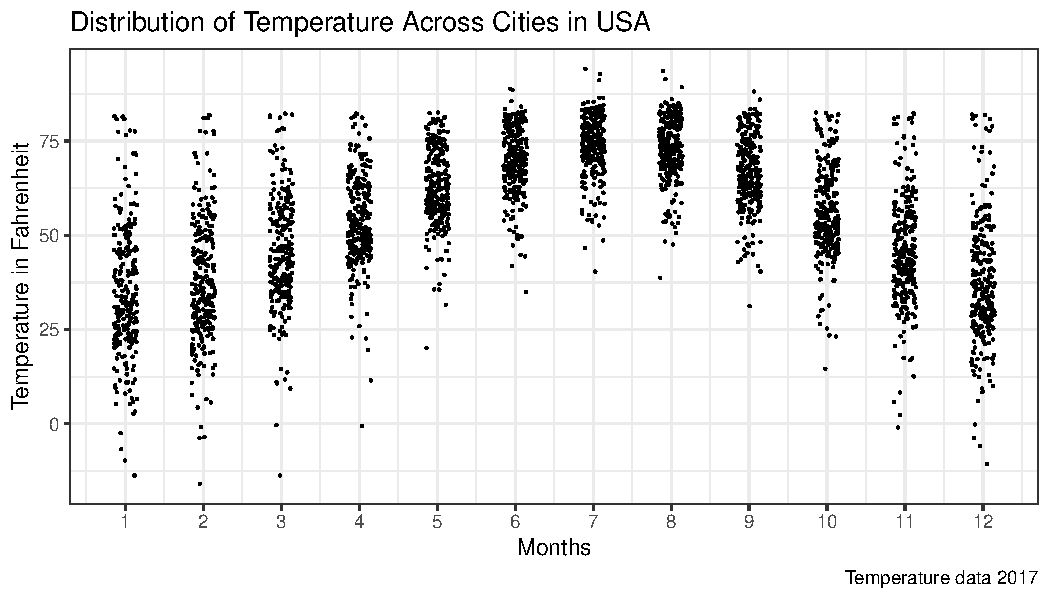
\includegraphics{Introductory-Statistics-with-R-tidyverse_files/figure-latex/unnamed-chunk-44-1} \end{center}

\hypertarget{scatter-plot-of-temperature-and-months-for-3-states}{%
\subsubsection{Scatter Plot of Temperature and Months for 3 States}\label{scatter-plot-of-temperature-and-months-for-3-states}}

Now, we will generate a similar chart as above, but let's select three states, and use different colors for each of the three states.

We can see that there are differences in average temperature across cities in each state in each month, but the different states also have different levels of variations in city temperatures within months.

We want to calculate both mean and standard deviations to capture both differences in averages over the year, as well as differences in how temperature varies within a month over the year.

\begin{Shaded}
\begin{Highlighting}[]
\CommentTok{\# Control Graph Size}
\KeywordTok{options}\NormalTok{(}\DataTypeTok{repr.plot.width =} \DecValTok{5}\NormalTok{, }\DataTypeTok{repr.plot.height =} \DecValTok{5}\NormalTok{)}
\CommentTok{\# First Filter Data}
\NormalTok{df\_temp\_txflak \textless{}{-}}\StringTok{ }\NormalTok{df\_temp }\OperatorTok{\%\textgreater{}\%}\StringTok{ }\KeywordTok{filter}\NormalTok{(state }\OperatorTok{\%in\%}\StringTok{ }\KeywordTok{c}\NormalTok{(}\StringTok{\textquotesingle{}AK\textquotesingle{}}\NormalTok{, }\StringTok{\textquotesingle{}TX\textquotesingle{}}\NormalTok{, }\StringTok{\textquotesingle{}FL\textquotesingle{}}\NormalTok{))}

\CommentTok{\# Draw Scatter Plot}
\CommentTok{\# 1. specify x and y}
\CommentTok{\# 2. label each state}
\CommentTok{\# 3. add in trend line}
\NormalTok{scatter \textless{}{-}}\StringTok{ }\KeywordTok{ggplot}\NormalTok{(df\_temp\_txflak, }\KeywordTok{aes}\NormalTok{(}\DataTypeTok{x=}\NormalTok{month, }\DataTypeTok{y=}\NormalTok{temp.f,}
                                      \DataTypeTok{colour=}\NormalTok{state)) }\OperatorTok{+}
\StringTok{      }\KeywordTok{geom\_jitter}\NormalTok{(}\DataTypeTok{size=}\DecValTok{1}\NormalTok{, }\DataTypeTok{width =} \FloatTok{0.15}\NormalTok{) }\OperatorTok{+}
\StringTok{      }\KeywordTok{labs}\NormalTok{(}\DataTypeTok{title =} \StringTok{\textquotesingle{}Distribution of Temperature Across Cities}\CharTok{\textbackslash{}n}\StringTok{in Florida (FL), Texas (TX) and Alaska (AK)\textquotesingle{}}\NormalTok{,}
           \DataTypeTok{x =} \StringTok{\textquotesingle{}Months\textquotesingle{}}\NormalTok{,}
           \DataTypeTok{y =} \StringTok{\textquotesingle{}Temperature in Fahrenheit\textquotesingle{}}\NormalTok{,}
           \DataTypeTok{caption =} \StringTok{\textquotesingle{}Temperature data 2017\textquotesingle{}}\NormalTok{) }\OperatorTok{+}
\StringTok{      }\KeywordTok{scale\_x\_continuous}\NormalTok{(}\DataTypeTok{labels =} \KeywordTok{as.character}\NormalTok{(df\_temp}\OperatorTok{$}\NormalTok{month),}
                         \DataTypeTok{breaks =}\NormalTok{ df\_temp}\OperatorTok{$}\NormalTok{month) }\OperatorTok{+}
\StringTok{      }\KeywordTok{theme\_bw}\NormalTok{()}
\KeywordTok{print}\NormalTok{(scatter)}
\end{Highlighting}
\end{Shaded}

\begin{center}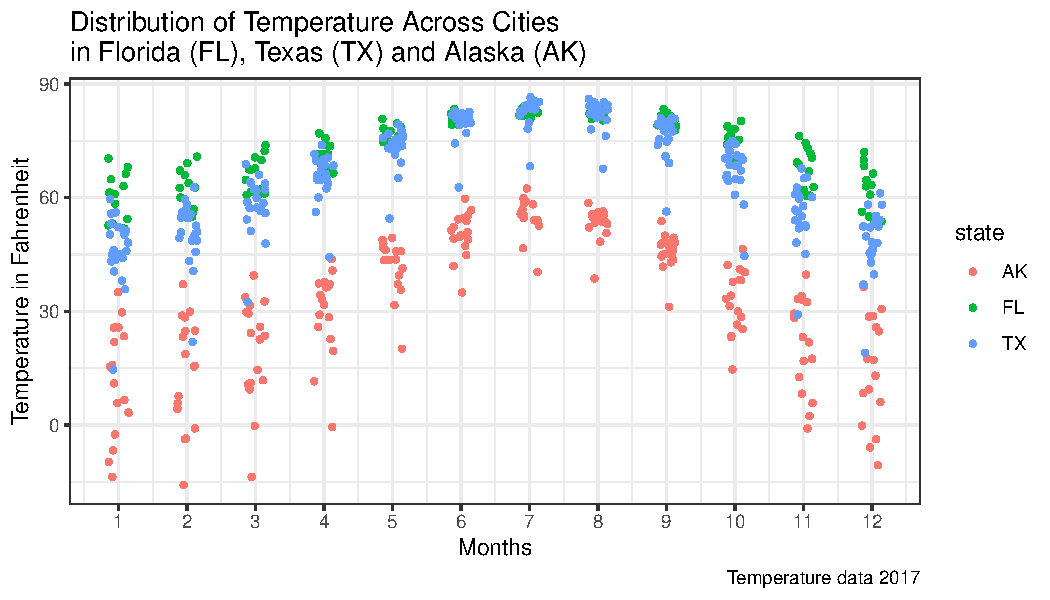
\includegraphics{Introductory-Statistics-with-R-tidyverse_files/figure-latex/unnamed-chunk-45-1} \end{center}

\hypertarget{mean-and-standard-deviation-within-month-acorss-usa}{%
\subsubsection{Mean and Standard Deviation Within Month Acorss USA}\label{mean-and-standard-deviation-within-month-acorss-usa}}

We can calculate the average temperature, as well as the standard deviation of temperature, in each month across cities in the USA. Let's show what these are using dplyr, and let's graph them out.

It's pretty amazing what mean, and standard deviation can do for us. We started with a dataset with many many observations, many many temperatures. Now with just 24 numbers below, we have created a way to summarize the large set of observations concisely. Twelve numbers for means for the 12 months, and 12 numbers for the standard deviations in 12 months.

This is like flying in the sky and taking a snapshot of the ground below from thousands of miles up.

The exciting thing here is, which statistics should we generate to adequately summarize what is going on on the ground within all the data observations? In this case here, if we show the mean, it informatively indicates that temperature is hotter during the summer, but it does not show the tightening of the temperature distribution during the summer months that we see in the scatter plot above. Adding standard deviation to our summary statistics, however, allows us also to see that as well.

\begin{Shaded}
\begin{Highlighting}[]
\CommentTok{\# Show mean and standard deviation in tabular form}
\NormalTok{df\_temp\_mth\_summ \textless{}{-}}\StringTok{ }\NormalTok{df\_temp }\OperatorTok{\%\textgreater{}\%}
\StringTok{    }\KeywordTok{group\_by}\NormalTok{(month) }\OperatorTok{\%\textgreater{}\%}
\StringTok{    }\KeywordTok{summarise}\NormalTok{(}\DataTypeTok{mean\_temp =} \KeywordTok{mean}\NormalTok{(temp.f), }\DataTypeTok{sd\_temp =} \KeywordTok{sd}\NormalTok{(temp.f))}
\end{Highlighting}
\end{Shaded}

\begin{Shaded}
\begin{Highlighting}[]
\CommentTok{\# Control Graph Size}
\KeywordTok{options}\NormalTok{(}\DataTypeTok{repr.plot.width =} \DecValTok{5}\NormalTok{, }\DataTypeTok{repr.plot.height =} \DecValTok{4}\NormalTok{)}
\CommentTok{\# Show mean and standard deviation in graphical form}
\CommentTok{\# We will gather the data first, it is an essential reshaping command}
\NormalTok{lineplot \textless{}{-}}\StringTok{ }\NormalTok{df\_temp\_mth\_summ }\OperatorTok{\%\textgreater{}\%}
\StringTok{    }\KeywordTok{gather}\NormalTok{(variable, value, }\OperatorTok{{-}}\NormalTok{month) }\OperatorTok{\%\textgreater{}\%}
\StringTok{    }\KeywordTok{ggplot}\NormalTok{(}\KeywordTok{aes}\NormalTok{(}\DataTypeTok{x=}\NormalTok{month, }\DataTypeTok{y=}\NormalTok{value, }\DataTypeTok{colour=}\NormalTok{variable, }\DataTypeTok{linetype=}\NormalTok{variable)) }\OperatorTok{+}
\StringTok{        }\KeywordTok{geom\_line}\NormalTok{() }\OperatorTok{+}
\StringTok{        }\KeywordTok{geom\_point}\NormalTok{() }\OperatorTok{+}
\StringTok{        }\KeywordTok{labs}\NormalTok{(}\DataTypeTok{title =} \StringTok{\textquotesingle{}Mean and SD of Temperature Acorss US Cities\textquotesingle{}}\NormalTok{,}
             \DataTypeTok{x =} \StringTok{\textquotesingle{}Months\textquotesingle{}}\NormalTok{,}
             \DataTypeTok{y =} \StringTok{\textquotesingle{}Temperature in Fahrenheit\textquotesingle{}}\NormalTok{,}
             \DataTypeTok{caption =} \StringTok{\textquotesingle{}Temperature data 2017\textquotesingle{}}\NormalTok{) }\OperatorTok{+}
\StringTok{        }\KeywordTok{scale\_x\_continuous}\NormalTok{(}\DataTypeTok{labels =} \KeywordTok{as.character}\NormalTok{(df\_temp\_mth\_summ}\OperatorTok{$}\NormalTok{month),}
                           \DataTypeTok{breaks =}\NormalTok{ df\_temp\_mth\_summ}\OperatorTok{$}\NormalTok{month)}
\KeywordTok{print}\NormalTok{(lineplot)}
\end{Highlighting}
\end{Shaded}

\begin{center}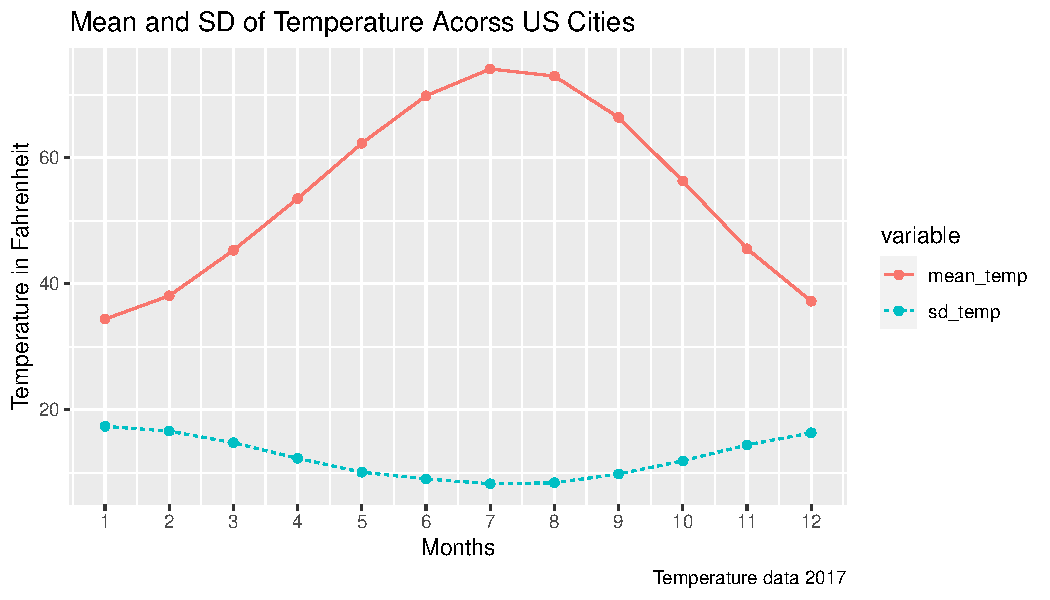
\includegraphics{Introductory-Statistics-with-R-tidyverse_files/figure-latex/unnamed-chunk-47-1} \end{center}

\hypertarget{mean-and-standard-deviation-within-month-acorss-states-in-usa}{%
\subsubsection{Mean and Standard Deviation Within Month Acorss States in USA}\label{mean-and-standard-deviation-within-month-acorss-states-in-usa}}

We have various states, how do these mean and sd charts vary across the big states that we have, where there are numerous cities in each state?

Let's generate some state-specific charts, using very simple commands below, and see how fascinating the United States is.

Specifically, we will have two charts:
1. the first chart has 4 subplots for each state showing the mean and sd for each state across months
2. the second chart has 2 subplots, showing inside each four lines for the four states.

\begin{Shaded}
\begin{Highlighting}[]
\CommentTok{\# Control Graph Size}
\KeywordTok{options}\NormalTok{(}\DataTypeTok{repr.plot.width =} \DecValTok{6}\NormalTok{, }\DataTypeTok{repr.plot.height =} \DecValTok{6}\NormalTok{)}
\CommentTok{\# Show mean and standard deviation in graphical form}
\CommentTok{\# We start from the dataset:}
\CommentTok{\# 1. select a subset of states we want}
\CommentTok{\# 2. group by state and month to generate mean and sd}
\CommentTok{\# 3. reshape data with gather}
\CommentTok{\# 4. generate line plots, state by state}

\NormalTok{lineplot \textless{}{-}}\StringTok{ }\NormalTok{df\_temp }\OperatorTok{\%\textgreater{}\%}
\StringTok{    }\KeywordTok{filter}\NormalTok{(state }\OperatorTok{\%in\%}\StringTok{ }\KeywordTok{c}\NormalTok{(}\StringTok{\textquotesingle{}AK\textquotesingle{}}\NormalTok{, }\StringTok{\textquotesingle{}CA\textquotesingle{}}\NormalTok{, }\StringTok{\textquotesingle{}FL\textquotesingle{}}\NormalTok{, }\StringTok{\textquotesingle{}TX\textquotesingle{}}\NormalTok{)) }\OperatorTok{\%\textgreater{}\%}
\StringTok{    }\KeywordTok{group\_by}\NormalTok{(state, month) }\OperatorTok{\%\textgreater{}\%}
\StringTok{    }\KeywordTok{summarise}\NormalTok{(}\DataTypeTok{mean\_temp =} \KeywordTok{mean}\NormalTok{(temp.f), }\DataTypeTok{sd\_temp =} \KeywordTok{sd}\NormalTok{(temp.f)) }\OperatorTok{\%\textgreater{}\%}
\StringTok{    }\KeywordTok{gather}\NormalTok{(variable, value, }\OperatorTok{{-}}\NormalTok{month, }\OperatorTok{{-}}\NormalTok{state) }\OperatorTok{\%\textgreater{}\%}
\StringTok{    }\KeywordTok{ggplot}\NormalTok{(}\KeywordTok{aes}\NormalTok{(}\DataTypeTok{x=}\NormalTok{month, }\DataTypeTok{y=}\NormalTok{value,}
               \DataTypeTok{colour=}\NormalTok{variable, }\DataTypeTok{linetype=}\NormalTok{variable, }\DataTypeTok{shape=}\NormalTok{variable)) }\OperatorTok{+}
\StringTok{        }\KeywordTok{facet\_wrap}\NormalTok{( }\OperatorTok{\textasciitilde{}}\StringTok{ }\NormalTok{state) }\OperatorTok{+}
\StringTok{        }\KeywordTok{geom\_line}\NormalTok{() }\OperatorTok{+}
\StringTok{        }\KeywordTok{geom\_point}\NormalTok{() }\OperatorTok{+}
\StringTok{        }\KeywordTok{labs}\NormalTok{(}\DataTypeTok{title =} \StringTok{\textquotesingle{}Mean and SD of Temperature Acorss US Cities\textquotesingle{}}\NormalTok{,}
             \DataTypeTok{x =} \StringTok{\textquotesingle{}Months\textquotesingle{}}\NormalTok{,}
             \DataTypeTok{y =} \StringTok{\textquotesingle{}Temperature in Fahrenheit\textquotesingle{}}\NormalTok{,}
             \DataTypeTok{caption =} \StringTok{\textquotesingle{}Temperature data 2017\textquotesingle{}}\NormalTok{) }\OperatorTok{+}
\StringTok{        }\KeywordTok{scale\_x\_continuous}\NormalTok{(}\DataTypeTok{labels =} \KeywordTok{as.character}\NormalTok{(df\_temp\_mth\_summ}\OperatorTok{$}\NormalTok{month),}
                           \DataTypeTok{breaks =}\NormalTok{ df\_temp\_mth\_summ}\OperatorTok{$}\NormalTok{month)}
\KeywordTok{print}\NormalTok{(lineplot)}
\end{Highlighting}
\end{Shaded}

\begin{center}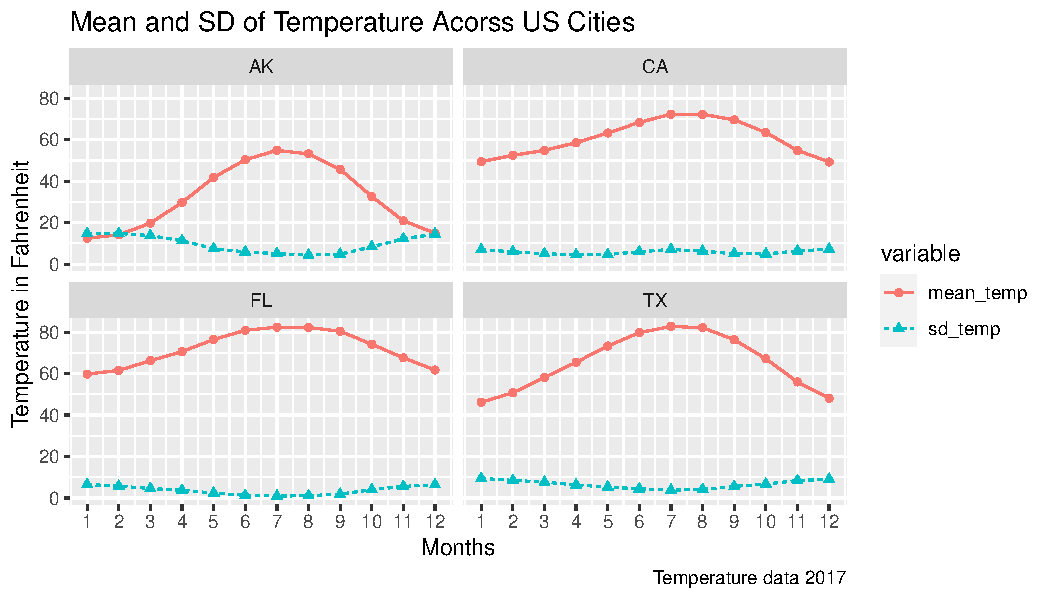
\includegraphics{Introductory-Statistics-with-R-tidyverse_files/figure-latex/unnamed-chunk-48-1} \end{center}

\begin{Shaded}
\begin{Highlighting}[]
\CommentTok{\# Control Graph Size}
\KeywordTok{options}\NormalTok{(}\DataTypeTok{repr.plot.width =} \DecValTok{6}\NormalTok{, }\DataTypeTok{repr.plot.height =} \DecValTok{4}\NormalTok{)}
\CommentTok{\# Show mean and standard deviation in graphical form}
\CommentTok{\# We start from the dataset:}
\CommentTok{\# 1. select a subset of states we want}
\CommentTok{\# 2. group by state and month to generate mean and sd}
\CommentTok{\# 3. reshape data with gather}
\CommentTok{\# 4. generate line plots, state by state}

\NormalTok{lineplot \textless{}{-}}\StringTok{ }\NormalTok{df\_temp }\OperatorTok{\%\textgreater{}\%}
\StringTok{    }\KeywordTok{filter}\NormalTok{(state }\OperatorTok{\%in\%}\StringTok{ }\KeywordTok{c}\NormalTok{(}\StringTok{\textquotesingle{}AK\textquotesingle{}}\NormalTok{, }\StringTok{\textquotesingle{}CA\textquotesingle{}}\NormalTok{, }\StringTok{\textquotesingle{}FL\textquotesingle{}}\NormalTok{, }\StringTok{\textquotesingle{}TX\textquotesingle{}}\NormalTok{)) }\OperatorTok{\%\textgreater{}\%}
\StringTok{    }\KeywordTok{group\_by}\NormalTok{(state, month) }\OperatorTok{\%\textgreater{}\%}
\StringTok{    }\KeywordTok{summarise}\NormalTok{(}\DataTypeTok{mean\_temp =} \KeywordTok{mean}\NormalTok{(temp.f), }\DataTypeTok{sd\_temp =} \KeywordTok{sd}\NormalTok{(temp.f)) }\OperatorTok{\%\textgreater{}\%}
\StringTok{    }\KeywordTok{gather}\NormalTok{(variable, value, }\OperatorTok{{-}}\NormalTok{month, }\OperatorTok{{-}}\NormalTok{state) }\OperatorTok{\%\textgreater{}\%}
\StringTok{    }\KeywordTok{ggplot}\NormalTok{(}\KeywordTok{aes}\NormalTok{(}\DataTypeTok{x=}\NormalTok{month, }\DataTypeTok{y=}\NormalTok{value,}
               \DataTypeTok{colour=}\NormalTok{state, }\DataTypeTok{linetype=}\NormalTok{state, }\DataTypeTok{shape=}\NormalTok{state)) }\OperatorTok{+}
\StringTok{        }\KeywordTok{facet\_wrap}\NormalTok{( }\OperatorTok{\textasciitilde{}}\StringTok{ }\NormalTok{variable, }\DataTypeTok{scales=}\StringTok{"free\_y"}\NormalTok{) }\OperatorTok{+}
\StringTok{        }\KeywordTok{geom\_line}\NormalTok{() }\OperatorTok{+}
\StringTok{        }\KeywordTok{geom\_point}\NormalTok{() }\OperatorTok{+}
\StringTok{        }\KeywordTok{labs}\NormalTok{(}\DataTypeTok{title =} \StringTok{\textquotesingle{}Mean and SD of Temperature Acorss US Cities\textquotesingle{}}\NormalTok{,}
             \DataTypeTok{x =} \StringTok{\textquotesingle{}Months\textquotesingle{}}\NormalTok{,}
             \DataTypeTok{y =} \StringTok{\textquotesingle{}Temperature in Fahrenheit\textquotesingle{}}\NormalTok{,}
             \DataTypeTok{caption =} \StringTok{\textquotesingle{}Temperature data 2017\textquotesingle{}}\NormalTok{) }\OperatorTok{+}
\StringTok{        }\KeywordTok{scale\_x\_continuous}\NormalTok{(}\DataTypeTok{labels =} \KeywordTok{as.character}\NormalTok{(df\_temp\_mth\_summ}\OperatorTok{$}\NormalTok{month),}
                           \DataTypeTok{breaks =}\NormalTok{ df\_temp\_mth\_summ}\OperatorTok{$}\NormalTok{month)}
\KeywordTok{print}\NormalTok{(lineplot)}
\end{Highlighting}
\end{Shaded}

\begin{center}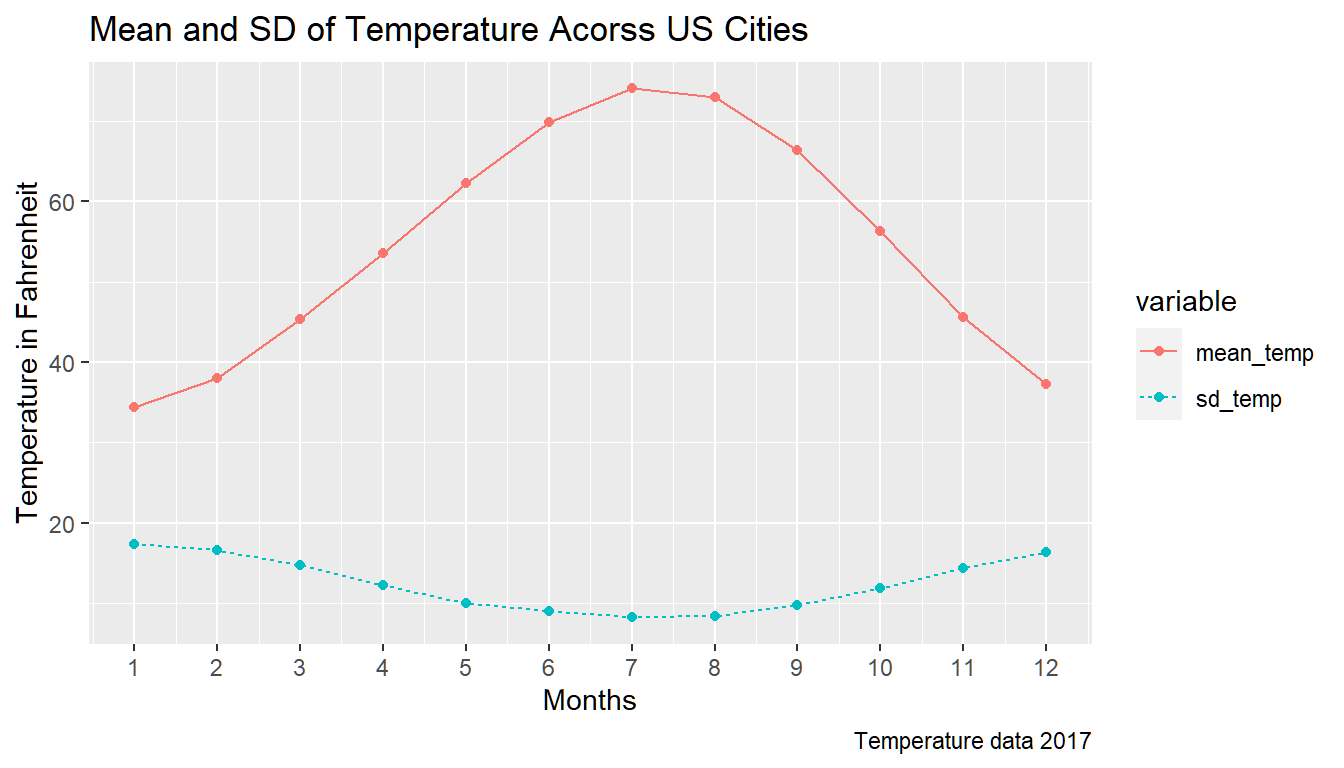
\includegraphics{Introductory-Statistics-with-R-tidyverse_files/figure-latex/unnamed-chunk-49-1} \end{center}

\hypertarget{coefficient-of-variation-and-correlation}{%
\section{Coefficient of Variation and Correlation}\label{coefficient-of-variation-and-correlation}}

\begin{quote}
Go back to \href{http://fanwangecon.github.io/}{fan}'s \href{https://fanwangecon.github.io/REconTools/}{REconTools} Package, \href{https://fanwangecon.github.io/R4Econ/}{R Code Examples} Repository (\href{https://fanwangecon.github.io/R4Econ/bookdown}{bookdown site}), or \href{https://fanwangecon.github.io/Stat4Econ/}{Intro Stats with R} Repository (\href{https://fanwangecon.github.io/Stat4Econ/bookdown}{bookdown site}).
\end{quote}

We have various tools at our disposal to summarize variables and the relationship between variables. Imagine that we have multiple toolboxes. This is the first one. There are two levels to this toolbox. Three Basic Tools:

\begin{enumerate}
\def\labelenumi{\arabic{enumi}.}
\tightlist
\item
  (sample) Mean of X (or Y)
\item
  (sample) Standard Deviation of X (or Y)
\item
  (sample) Covariance of X and Y
\end{enumerate}

Additionally, we have two tools that combine the tools from the first level:

\begin{enumerate}
\def\labelenumi{\arabic{enumi}.}
\tightlist
\item
  Coefficient of Variation = (Standard Deviation)/(Mean)
\item
  Correlation = (Covariance of X and Y)/((Standard Deviation of X)*(Standard Deviation of Y))
\end{enumerate}

The tools on the second level rescale the standard deviation and covariance statistics.

\hypertarget{education-and-wage}{%
\subsection{Education and Wage}\label{education-and-wage}}

The dataset, \emph{EPIStateEduWage2017.csv}, can be downloaded \href{https://github.com/FanWangEcon/Stat4Econ/tree/master/data/EPIStateEduWage2017.csv}{here}.

Two variables:

\begin{enumerate}
\def\labelenumi{\arabic{enumi}.}
\tightlist
\item
  Fraction of individual with college degree in a state

  \begin{itemize}
  \tightlist
  \item
    this is in Fraction units, the minimum is 0.00, the maximum is 100 percent, which is 1.00
  \end{itemize}
\item
  Average hourly salary in the state

  \begin{itemize}
  \tightlist
  \item
    this is in Dollar units
  \end{itemize}
\end{enumerate}

\begin{Shaded}
\begin{Highlighting}[]
\CommentTok{\# Load in Data Tools}
\CommentTok{\# For Reading/Loading Data}
\KeywordTok{library}\NormalTok{(readr)}
\KeywordTok{library}\NormalTok{(tibble)}
\KeywordTok{library}\NormalTok{(dplyr)}
\KeywordTok{library}\NormalTok{(ggplot2)}
\CommentTok{\# Load in Data}
\NormalTok{df\_wgedu \textless{}{-}}\StringTok{ }\KeywordTok{read\_csv}\NormalTok{(}\StringTok{\textquotesingle{}data/EPIStateEduWage2017.csv\textquotesingle{}}\NormalTok{)}
\end{Highlighting}
\end{Shaded}

\hypertarget{a-scatter-plot}{%
\subsubsection{A Scatter Plot}\label{a-scatter-plot}}

We can Visualize the Data with a Scatter Plot. There seems to be a positive relationship between the share of individuals in a state with a college education, and the average hourly salary in that state.

While most states are along the trend line, we have some states, like WY, that are outliers. WY has a high hourly salary but low share with college education.

\begin{Shaded}
\begin{Highlighting}[]
\CommentTok{\# Control Graph Size}
\KeywordTok{options}\NormalTok{(}\DataTypeTok{repr.plot.width =} \DecValTok{5}\NormalTok{, }\DataTypeTok{repr.plot.height =} \DecValTok{5}\NormalTok{)}
\CommentTok{\# Draw Scatter Plot}
\CommentTok{\# 1. specify x and y}
\CommentTok{\# 2. label each state}
\CommentTok{\# 3. add in trend line}
\NormalTok{scatter \textless{}{-}}\StringTok{ }\KeywordTok{ggplot}\NormalTok{(df\_wgedu, }\KeywordTok{aes}\NormalTok{(}\DataTypeTok{x=}\NormalTok{Share.College.Edu, }\DataTypeTok{y=}\NormalTok{Hourly.Salary)) }\OperatorTok{+}
\StringTok{      }\KeywordTok{geom\_point}\NormalTok{(}\DataTypeTok{size=}\DecValTok{1}\NormalTok{) }\OperatorTok{+}
\StringTok{      }\KeywordTok{geom\_text}\NormalTok{(}\KeywordTok{aes}\NormalTok{(}\DataTypeTok{label=}\NormalTok{State), }\DataTypeTok{size=}\DecValTok{3}\NormalTok{, }\DataTypeTok{hjust=}\OperatorTok{{-}}\NormalTok{.}\DecValTok{2}\NormalTok{, }\DataTypeTok{vjust=}\OperatorTok{{-}}\NormalTok{.}\DecValTok{2}\NormalTok{) }\OperatorTok{+}
\StringTok{      }\KeywordTok{geom\_smooth}\NormalTok{(}\DataTypeTok{method=}\NormalTok{lm) }\OperatorTok{+}
\StringTok{      }\KeywordTok{labs}\NormalTok{(}\DataTypeTok{title =} \StringTok{\textquotesingle{}Hourly Wage and College Share by States\textquotesingle{}}\NormalTok{,}
           \DataTypeTok{x =} \StringTok{\textquotesingle{}Fraction with College Education\textquotesingle{}}\NormalTok{,}
           \DataTypeTok{y =} \StringTok{\textquotesingle{}Hourly Wage\textquotesingle{}}\NormalTok{,}
           \DataTypeTok{caption =} \StringTok{\textquotesingle{}Economic Policy Institute}\CharTok{\textbackslash{}n}\StringTok{ www.epi.org/data/\textquotesingle{}}\NormalTok{) }\OperatorTok{+}
\StringTok{      }\KeywordTok{theme\_bw}\NormalTok{()}
\KeywordTok{print}\NormalTok{(scatter)}
\end{Highlighting}
\end{Shaded}

\begin{center}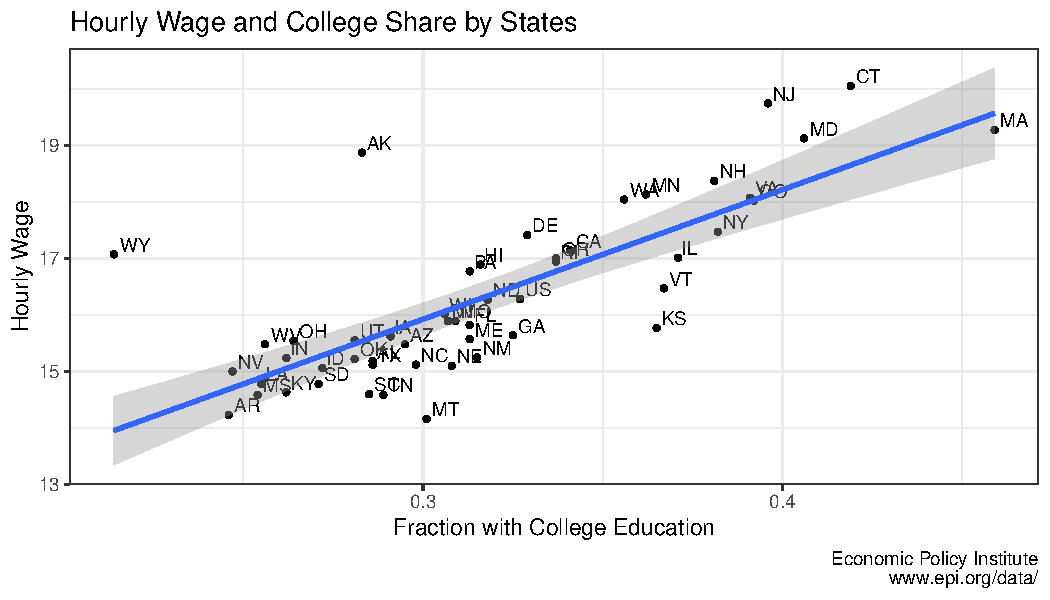
\includegraphics{Introductory-Statistics-with-R-tidyverse_files/figure-latex/unnamed-chunk-52-1} \end{center}

\hypertarget{standard-deviations-and-coefficient-of-variation}{%
\subsubsection{Standard Deviations and Coefficient of Variation}\label{standard-deviations-and-coefficient-of-variation}}

The two variables above are in different units. We first calculate the mean, standard deviation, and covariance. With just these, it is hard to compare the standard deviation of the two variables, which are on different scales.

The sample standard deviations for the two variables are: \(0.051\) and \(1.51\), in fraction and dollar units. Can we say the hourly salary has a larger standard deviation? But it is just a different scale. \(1.51\) is a large number, but that does not mean that variable has greater variation than the fraction with college education variable.

Converting the Statistics to Coefficient of Variations, now we have: \(0.16\) and \(0.09\). Because of the division, these are both in fraction units--standard deviations as a fraction of the mean. Now these are more comparable.

\begin{Shaded}
\begin{Highlighting}[]
\CommentTok{\# We can compute the three basic statistics}
\NormalTok{stats.msdv \textless{}{-}}\StringTok{ }\KeywordTok{list}\NormalTok{(}
              \CommentTok{\# Mean, SD and Var for the College Share variable}
              \DataTypeTok{Shr.Coll.Mean =} \KeywordTok{mean}\NormalTok{(df\_wgedu}\OperatorTok{$}\NormalTok{Share.College.Edu),}
              \DataTypeTok{Shr.Coll.Std =} \KeywordTok{sd}\NormalTok{(df\_wgedu}\OperatorTok{$}\NormalTok{Share.College.Edu),}
              \DataTypeTok{Shr.Coll.Var =} \KeywordTok{var}\NormalTok{(df\_wgedu}\OperatorTok{$}\NormalTok{Share.College.Edu),}

              \CommentTok{\# Mean, SD and Var for the Hourly Wage Variable}
              \DataTypeTok{Hr.Wage.Mean =} \KeywordTok{mean}\NormalTok{(df\_wgedu}\OperatorTok{$}\NormalTok{Hourly.Salary),}
              \DataTypeTok{Hr.Wage.Std =} \KeywordTok{sd}\NormalTok{(df\_wgedu}\OperatorTok{$}\NormalTok{Hourly.Salary),}
              \DataTypeTok{Hr.Wage.Var =} \KeywordTok{var}\NormalTok{(df\_wgedu}\OperatorTok{$}\NormalTok{Hourly.Salary)}
\NormalTok{              )}

\CommentTok{\# We can compute the three basic statistics}
\NormalTok{stats.coefvari \textless{}{-}}\StringTok{ }\KeywordTok{list}\NormalTok{(}
              \CommentTok{\# Coefficient of Variation}
              \DataTypeTok{Shr.Coll.Coef.Variation =}\NormalTok{ (stats.msdv}\OperatorTok{$}\NormalTok{Shr.Coll.Std)}\OperatorTok{/}\NormalTok{(stats.msdv}\OperatorTok{$}\NormalTok{Shr.Coll.Mean),}
              \DataTypeTok{Hr.Wage.Coef.Variation =}\NormalTok{ (stats.msdv}\OperatorTok{$}\NormalTok{Hr.Wage.Std)}\OperatorTok{/}\NormalTok{(stats.msdv}\OperatorTok{$}\NormalTok{Hr.Wage.Mean)}
\NormalTok{              )}

\CommentTok{\# Let\textquotesingle{}s Print the Statistics we Computed}
\KeywordTok{as\_tibble}\NormalTok{(stats.msdv)}
\KeywordTok{as\_tibble}\NormalTok{(stats.coefvari)}
\end{Highlighting}
\end{Shaded}

\hypertarget{covariance-and-correlation}{%
\subsubsection{Covariance and Correlation}\label{covariance-and-correlation}}

For covariance, hard to tell whether it is large or small. To make comparisons possible, we calculate the coefficient of variations and correlation statistics.

The covariance we get is positive: \(0.06\), but is this actually large positive relationship? \(0.06\) seems like a small number.

Rescaling covariance to correlation, the correlation between the two variables is: \(0.78\). Since the correlation of two variable is below \(-1\) and \(+1\), we can now say actually the two variables are very positively related. A higher share of individuals with a college education is strongly positively correlated with a higher hourly salary.

\begin{Shaded}
\begin{Highlighting}[]
\CommentTok{\# We can compute the three basic statistics}
\NormalTok{states.covcor \textless{}{-}}\StringTok{ }\KeywordTok{list}\NormalTok{(}
              \CommentTok{\# Covariance between the two variables}
              \DataTypeTok{Shr.Wage.Cov =} \KeywordTok{cov}\NormalTok{(df\_wgedu}\OperatorTok{$}\NormalTok{Hourly.Salary,}
\NormalTok{                                 df\_wgedu}\OperatorTok{$}\NormalTok{Share.College.Edu),}
              \CommentTok{\# Correlation}
              \DataTypeTok{Shr.Wage.Cor =} \KeywordTok{cor}\NormalTok{(df\_wgedu}\OperatorTok{$}\NormalTok{Hourly.Salary, df\_wgedu}\OperatorTok{$}\NormalTok{Share.College.Edu),}
              \DataTypeTok{Shr.Wage.Cor.Formula =}\NormalTok{ (}\KeywordTok{cov}\NormalTok{(df\_wgedu}\OperatorTok{$}\NormalTok{Hourly.Salary, df\_wgedu}\OperatorTok{$}\NormalTok{Share.College.Edu)}
                                      \OperatorTok{/}\NormalTok{(stats.msdv}\OperatorTok{$}\NormalTok{Shr.Coll.Std}\OperatorTok{*}\NormalTok{stats.msdv}\OperatorTok{$}\NormalTok{Hr.Wage.Std))}
\NormalTok{              )}

\CommentTok{\# Let\textquotesingle{}s Print the Statistics we Computed}
\KeywordTok{as\_tibble}\NormalTok{(states.covcor)}
\end{Highlighting}
\end{Shaded}

\hypertarget{basics-of-probability}{%
\chapter{Basics of Probability}\label{basics-of-probability}}

\hypertarget{experimental-outcomes}{%
\section{Experimental Outcomes}\label{experimental-outcomes}}

\begin{quote}
Go back to \href{http://fanwangecon.github.io/}{fan}'s \href{https://fanwangecon.github.io/REconTools/}{REconTools} Package, \href{https://fanwangecon.github.io/R4Econ/}{R Code Examples} Repository (\href{https://fanwangecon.github.io/R4Econ/bookdown}{bookdown site}), or \href{https://fanwangecon.github.io/Stat4Econ/}{Intro Stats with R} Repository (\href{https://fanwangecon.github.io/Stat4Econ/bookdown}{bookdown site}).
\end{quote}

\begin{enumerate}
\def\labelenumi{\arabic{enumi}.}
\tightlist
\item
  Experiment

  \begin{itemize}
  \tightlist
  \item
    ``We define an experiment as a process that generates well-defined outcomes'' (ASWCC P171)
  \end{itemize}
\item
  Sample Space

  \begin{itemize}
  \tightlist
  \item
    ``The sample space for an experiment is the set of all experimental outcomes'' (ASWCC P172)
  \end{itemize}
\item
  Experimental outcomes

  \begin{itemize}
  \tightlist
  \item
    ``An experimental outcome is also called a sample point to identify it as an element of the sample space.'' (ASWCC P172)
  \end{itemize}
\item
  Events

  \begin{itemize}
  \tightlist
  \item
    ``An Event is a collection of Sample Points'' (AWSCC P181), could be just one sample point (one experimental outcome)
  \end{itemize}
\item
  Probability

  \begin{itemize}
  \tightlist
  \item
    ``Probability is a numerical measure of the likelihood that an event will occur.'' (AWSCC P171)
  \end{itemize}
\end{enumerate}

\hypertarget{sample-space-and-probabilities}{%
\subsection{Sample Space and Probabilities}\label{sample-space-and-probabilities}}

\textbf{Sample Space and Experimental Outcomes}

We can use the letter \(S\) or \(\Omega\) to denote sample space. Supose we have a set of \(n\) experimental outcomes:

\[S = \left\{ E_1, E_2, ..., E_{n-1}, E_n\right\}\]

We can call \(S\) a sample space if:

\begin{enumerate}
\def\labelenumi{\arabic{enumi}.}
\tightlist
\item
  \(E_i\) are mutually exclusive:

  \begin{itemize}
  \tightlist
  \item
    \(E_i\) for all \(i\) are separate outcomes that do not overlap.
  \item
    Suppose there are multiple people running for the Presidency, some of these candidates are women, and some of these women are from Texas. If one of the \(E_i\) is that a woman becomes the President, and another \(E_i\) is that someone from Texas becomes the President, \(S\) would not be a sample space, because we could have a woman who is also from Texas win the Presidency.
  \end{itemize}
\item
  \(E_i\) are jointly exhaustive:

  \begin{itemize}
  \tightlist
  \item
    For the experiment with well-defined outcomes, the \(E_i\) in \(S\) need to cover all possible outcomes.
  \item
    If you are throwing a six sided dice, there are six possible experimental outcomes, if \(S\) only has five of them, it would not be a sample space.
  \end{itemize}
\end{enumerate}

Thinking about the world in terms of sample space is pretty amazing.

\textbf{Assigning Probability to Experimental Outcomes}

We can assign probabilities to events of a sample space. Since experimental outcomes are themselves events as well, we can assign probabilities to each experimental outcome.

For the mutually exclusive and jointly exhaustive experimental outcomes of the sample space, there are two equirements for assigning probabilities:
- Each element of the sample space can not have negative probability of happening, and also can not have more than \(1\) probability of happening, with \(P\) denotes probability, we have:
\[0 \le P(E_i) \le 1\]
- The probabilities of all the mutually exclusive and jointly exhaustive experimental outcomes in the sample space sum up to \(1\). For an experimental with \(n\) experimental outcomes:
\[\Sigma_{i=1}^{n} P(E_i) = 1\]

\begin{Shaded}
\begin{Highlighting}[]
\CommentTok{\# Load Library}
\KeywordTok{library}\NormalTok{(tidyverse)}

\CommentTok{\# Define a List of Experimental Outcomes}
\NormalTok{experimental.outcomes.list \textless{}{-}}\StringTok{ }\KeywordTok{c}\NormalTok{(}\StringTok{\textquotesingle{}Heavy Rain\textquotesingle{}}\NormalTok{, }\StringTok{\textquotesingle{}Light Rain\textquotesingle{}}\NormalTok{, }\StringTok{\textquotesingle{}No Rain\textquotesingle{}}\NormalTok{)}

\CommentTok{\# Probabilities on experimental outcomes}
\NormalTok{experimental.outcome.prob \textless{}{-}}\StringTok{ }\KeywordTok{c}\NormalTok{(}\FloatTok{0.1}\NormalTok{, }\FloatTok{0.2}\NormalTok{, }\FloatTok{0.7}\NormalTok{)}

\CommentTok{\# Show these in a Tibble}
\KeywordTok{tibble}\NormalTok{(}\DataTypeTok{tomorrow.experimental.outcomes =}\NormalTok{ experimental.outcomes.list,}
       \DataTypeTok{experimental.outcome.prob =}\NormalTok{ experimental.outcome.prob)}
\end{Highlighting}
\end{Shaded}

\begin{Shaded}
\begin{Highlighting}[]
\CommentTok{\# What could happen tomorrow?}
\CommentTok{\# We live in a probabilistic world, from today\textquotesingle{}s perspective, tomorrow is uncertain}
\CommentTok{\# If we draw tomorrow from a hat, given our possible outcomes}
\CommentTok{\# and the probabilities associated with the outcomes}
\CommentTok{\# what are the possible tomorrows?}
\NormalTok{number.of.tomorrow.to.draw =}\StringTok{ }\DecValTok{20}
\NormalTok{tomorrow.weather.draws \textless{}{-}}\StringTok{ }\KeywordTok{sample}\NormalTok{(experimental.outcomes.list,}
                                 \DataTypeTok{size =}\NormalTok{ number.of.tomorrow.to.draw,}
                                 \DataTypeTok{replace =} \OtherTok{TRUE}\NormalTok{,}
                                 \DataTypeTok{prob =}\NormalTok{ experimental.outcome.prob)}

\CommentTok{\# A little tibble to show results}
\CommentTok{\# There are only three unique tomorrows, each of three weather outcomes}
\CommentTok{\# could happen, but the chance of each happening differs by the probabilities}
\CommentTok{\# we set in experimental.outcome.prob}
\KeywordTok{tibble}\NormalTok{(}\DataTypeTok{which.tomorrow =} \KeywordTok{paste0}\NormalTok{(}\StringTok{\textquotesingle{}tomorrow:\textquotesingle{}}\NormalTok{, }\DecValTok{1}\OperatorTok{:}\NormalTok{number.of.tomorrow.to.draw),}
       \DataTypeTok{tomorrow.weather =}\NormalTok{ tomorrow.weather.draws)}
\end{Highlighting}
\end{Shaded}

\hypertarget{union-and-intersection-and-complements}{%
\subsection{Union and Intersection and Complements}\label{union-and-intersection-and-complements}}

Definitions:

\begin{enumerate}
\def\labelenumi{\arabic{enumi}.}
\tightlist
\item
  Complement of Event \(A\):

  \begin{itemize}
  \tightlist
  \item
    ``Given an event A, the complement of A is defined to be the event consisting of all sample points that are not in A. The complement of A is denoted by \(A^c\).'' (AWSCC P185)
  \end{itemize}
\item
  The Union of Events \(A\) and \(B\):

  \begin{itemize}
  \tightlist
  \item
    ``The union of A and B is the event containing all sample points belonging to \(A\) or \(B\) or both. The union is denoted by \(A \cup B\).'' (AWSCC P186)
  \end{itemize}
\item
  The Intersection of Events \(A\) and \(B\):

  \begin{itemize}
  \tightlist
  \item
    ``Given two events \(A\) and \(B\), the intersection of \(A\) and \(B\) is the event containing the sample points belonging to both \(A\) and \(B\). The intersection is denoted by \(A \cap B\).'' (AWSCC P187)
  \end{itemize}
\end{enumerate}

\textbf{Probabilities for Complements and Union}

The Probabilities of Complements add up to 1:
\[P(A) + P(A^c) = 1\]

The \textbf{Addition Law}:
\[P (A \cup B) = P(A) + P(B) - P (A \cap B)\]

If two events \(A\) and \(B\) are mutually exclusive, which means they do not share any experimental outcomes (sample points), then: \(P (A \cap B) = 0\), and \(P (A \cup B) = P(A) + P(B)\).

The \textbf{Multiplication Law for Indepedent Events}:
\[P (A \cap B) = P(A) \cdot P(B)\]

If the probability of event \(A\) happening does not change the probability of event \(B\) happening, and vice-versa. The two events are independent. Below we arrive this formulation from conditional probability.

\hypertarget{conditional-probability}{%
\subsection{Conditional Probability}\label{conditional-probability}}

We use a straight line \(\mid\) to denote conditional probability. Given \(A\) happens, what is the probability of \(B\) happening?

\[P (A \mid B) = \frac{P(A \cap B)}{P(B)}\]

This says the probability of \(A\) happening given that \(B\) happens is equal to the ratio of the probability that both \(A\) and \(B\) happen divided by the probability of \(B\) happening.

The formula also means that the probability that both \(A\) and \(B\) happens is equal to the probability that \(B\) happens times the probability that \(A\) happens conditional on \(B\) happening:
\[ P(A \cap B) = P (A \mid B)\cdot P(B)\]

If \(A\) and \(B\) are independent, that means the probability of \(A\) happening does not change whether \(B\) happens or not, then, \(P (A \mid B) = P(A)\), and:
\[ \text{If A and B are independent: } P(A \cap B) = P(A) \cdot P(B)\]
This is what we wrote down earlier as well.

\hypertarget{sample-space-and-probability-examples}{%
\section{Sample Space and Probability Examples}\label{sample-space-and-probability-examples}}

\begin{quote}
Go back to \href{http://fanwangecon.github.io/}{fan}'s \href{https://fanwangecon.github.io/REconTools/}{REconTools} Package, \href{https://fanwangecon.github.io/R4Econ/}{R Code Examples} Repository (\href{https://fanwangecon.github.io/R4Econ/bookdown}{bookdown site}), or \href{https://fanwangecon.github.io/Stat4Econ/}{Intro Stats with R} Repository (\href{https://fanwangecon.github.io/Stat4Econ/bookdown}{bookdown site}).
\end{quote}

In \emph{\href{https://fanwangecon.github.io/Stat4Econ/probability/htmlpdfr/samplespace.html}{Sample Space, Experimental Outcomes, Events, Probabilities}}, we discussed various definitions. Here are some examples.

\begin{itemize}
\tightlist
\item
  Experiment: Throwing a Quarter
\item
  Experimental outcomes: lands on Heads or lands on Tails
\item
  Sample Space: \(S=\left\{H, T\right\}\)
\item
  Event: There are only two experimental outcomes.
\item
  Probability:

  \begin{itemize}
  \tightlist
  \item
    \(1 \ge P(H) \ge 0\)
  \item
    \(1 \ge P(T) \ge 0\)
  \item
    \(P(H) + P(T) = 1\)
  \end{itemize}
\end{itemize}

\hypertarget{presidential-election}{%
\subsection{Presidential Election}\label{presidential-election}}

After various primaries there are four major candidates who could become president. Voting takes place in half a year. Over this year, many events could happen that would increase or decrease the support for candidates. After voting, the outcome is certain. But from today's perspective, when voting is one year from now, outcomes are uncertain.

\begin{itemize}
\tightlist
\item
  Experiment: Presidential Election in One Year
\item
  Experimental outcomes: candidates \href{https://en.wikipedia.org/wiki/Donald_Trump}{DT}, \href{https://en.wikipedia.org/wiki/Hillary_Clinton}{HC}, \href{https://en.wikipedia.org/wiki/Jill_Stein}{JS}, \href{https://en.wikipedia.org/wiki/Gary_Johnson}{GJ} winning.
\item
  Sample Space: \{DT, HC, JS, GJ\}
\item
  Event:

  \begin{itemize}
  \tightlist
  \item
    A woman wins is an event: \(\text{W} = \left\{HC, JS\right\}\)
  \item
    A man wins: \(\text{M} = \left\{DT, GJ\right\}\)
  \item
    Someone from a small party wins: \(\text{S} = \left\{JS, GJ\right\}\)
  \end{itemize}
\item
  Probability:

  \begin{itemize}
  \tightlist
  \item
    The probability that a woman does not win:
    \[P(\text{W}^c) = 1 - P(\text{W}) = P(\text{M})\]
  \item
    There are no experimental outcomes, given the four that we have, where both woman and man wins, the two events are mutually exclusive:
    \[P(\text{W} \cap \text{M}) = 0\]
  \item
    The probability that a woman wins conditional on a man winnning is zero:
    \[P(\text{W} \mid \text{M}) = \frac{P(\text{W} \cap \text{M})}{P(\text{M})} = \frac{0}{P(DT) + P(GJ)} = 0\]
  \item
    The probability that a woman wins and someone from a small party wins:
    \[P(\text{W} \cap \text{S}) = P(JS)\]
  \item
    The probability that a woman wins conditional on someone from a small party winning:
    \[P(\text{W} \mid \text{S}) = \frac{P(\text{W} \cap \text{S})}{P(\text{S})} = \frac{P(JS)}{P(JS) + P(GJ)} \]
  \item
    Either a women wins or someone from a small party wins:
    \[P(\text{W} \cup \text{S}) = P(\text{W}) + P(\text{S}) - P(\text{W} \cap \text{S}) = P(HC) + P(JS) + P(JS) + P(GJ) - P(JS) =  P(HC) + P(JS) + P(GJ)\]
  \end{itemize}
\end{itemize}

\hypertarget{throwing-a-dice}{%
\subsection{Throwing a Dice}\label{throwing-a-dice}}

\begin{itemize}
\tightlist
\item
  Experiment: Throwing a Dice
\item
  Experimental outcomes: lands on one of the six sides
\item
  Sample Space: \(S=\left\{1,2,3,4,5,6\right\}\)
\item
  Event: One could define many possible events. The experimental outcome is less than 3 is an event, greater than 2 is an event, been odd is an event, etc.
\end{itemize}

In \href{https://fanwangecon.github.io/Stat4Econ/probability/htmlpdfr/samplespacedice.html}{Throw an Unfair Four Sided Dice}, we show what happens when we throw an unfair four sided dice many times. In the example below, we will throw an unfair dice, where the probability of landing on the side with 1 is 50 percent, and the chance of landing on each successive side is half of the chance of landing on the previous side. This is a dice weighted towards the smaller numbers.

See the table below for the true probabilities of the unfiar dice.

\begin{Shaded}
\begin{Highlighting}[]
\CommentTok{\# Load Library}
\KeywordTok{library}\NormalTok{(tidyverse)}

\CommentTok{\# Define a List of Experimental Outcomes}
\NormalTok{experimental.outcomes.list \textless{}{-}}\StringTok{ }\KeywordTok{c}\NormalTok{(}\DecValTok{1}\NormalTok{,}\DecValTok{2}\NormalTok{,}\DecValTok{3}\NormalTok{,}\DecValTok{4}\NormalTok{,}\DecValTok{5}\NormalTok{,}\DecValTok{6}\NormalTok{)}

\CommentTok{\# Probabilities on experimental outcomes}
\CommentTok{\# Suppose dice is weighted towards 1}
\NormalTok{fracbase \textless{}{-}}\StringTok{ }\FloatTok{0.50}
\NormalTok{experimental.outcome.prob \textless{}{-}}\StringTok{ }\KeywordTok{c}\NormalTok{((}\DecValTok{1}\OperatorTok{{-}}\NormalTok{fracbase)}\OperatorTok{\^{}}\DecValTok{0}\OperatorTok{*}\NormalTok{fracbase,}
\NormalTok{                               (}\DecValTok{1}\OperatorTok{{-}}\NormalTok{fracbase)}\OperatorTok{\^{}}\DecValTok{1}\OperatorTok{*}\NormalTok{fracbase,}
\NormalTok{                               (}\DecValTok{1}\OperatorTok{{-}}\NormalTok{fracbase)}\OperatorTok{\^{}}\DecValTok{2}\OperatorTok{*}\NormalTok{fracbase,}
\NormalTok{                               (}\DecValTok{1}\OperatorTok{{-}}\NormalTok{fracbase)}\OperatorTok{\^{}}\DecValTok{3}\OperatorTok{*}\NormalTok{fracbase,}
\NormalTok{                               (}\DecValTok{1}\OperatorTok{{-}}\NormalTok{fracbase)}\OperatorTok{\^{}}\DecValTok{4}\OperatorTok{*}\NormalTok{fracbase,}
\NormalTok{                               (}\DecValTok{1}\OperatorTok{{-}}\NormalTok{fracbase)}\OperatorTok{\^{}}\DecValTok{5}\NormalTok{)}

\CommentTok{\# Show these in a Tibble}
\NormalTok{dice.true.prob \textless{}{-}}\StringTok{ }\KeywordTok{tibble}\NormalTok{(}\DataTypeTok{dice.outcomes.list =}\NormalTok{ experimental.outcomes.list,}
                         \DataTypeTok{dice.true.prob =}\NormalTok{ experimental.outcome.prob)}
\NormalTok{dice.true.prob}
\end{Highlighting}
\end{Shaded}

\hypertarget{throw-the-dice-10-times}{%
\subsubsection{Throw the Dice 10 Times}\label{throw-the-dice-10-times}}

We throw the dice 10 times, each time, get one of the six possible experimental outcomes, the chance of getting these outcomes are determined by the true probabilities of the unfair dice. If we throw 10 times, that does not mean we will get exact side 1 five times. Side 1 having proability of 50 percent means for each throw there is a 50 percent chance of getting side 1. But each throw is independent of other throws, so we could just by chance end up with no side 1 after ten throws, although the chance of that happening is low. How many times did we get each side in the ten random tosses below?

\begin{Shaded}
\begin{Highlighting}[]
\CommentTok{\# What could happen tomorrow?}
\CommentTok{\# We live in a probabilistic world, drawing future from a hat}
\CommentTok{\# If we draw 20 times, what happens in the future?}
\CommentTok{\# It\textquotesingle{}s pretty amazing, we get to see the future!}
\NormalTok{number.of.futures.to.draw =}\StringTok{ }\DecValTok{10}
\NormalTok{future.dice.draws \textless{}{-}}\StringTok{ }\KeywordTok{sample}\NormalTok{(experimental.outcomes.list,}
                            \DataTypeTok{size =}\NormalTok{ number.of.futures.to.draw,}
                            \DataTypeTok{replace =} \OtherTok{TRUE}\NormalTok{,}
                            \DataTypeTok{prob =}\NormalTok{ experimental.outcome.prob)}

\CommentTok{\# A little tibble to show results}
\KeywordTok{tibble}\NormalTok{(}\DataTypeTok{which.future.dice =} \KeywordTok{paste0}\NormalTok{(}\StringTok{\textquotesingle{}dice draws:\textquotesingle{}}\NormalTok{, }\DecValTok{1}\OperatorTok{:}\NormalTok{number.of.futures.to.draw),}
       \DataTypeTok{dice.draws =}\NormalTok{ future.dice.draws)}
\end{Highlighting}
\end{Shaded}

\hypertarget{redefining-sample-space-for-throwing-a-dice}{%
\subsubsection{Redefining Sample Space for Throwing a Dice}\label{redefining-sample-space-for-throwing-a-dice}}

Following our definition for sample space above, we can actually define an alternative sample spaces, for example:

\begin{itemize}
\tightlist
\item
  Experiment: Throwing a Dice
\item
  Experimental outcomes: lands on greater or equal to 4, lands on less or equal to 3
\item
  Sample Space: \(S=\left\{\text{'less equal to 3'}, \text{'greater equal to 4'}\right\}\)
\end{itemize}

This is also a sample space with two sample points (or experimental outcomes). Following our \href{https://fanwangecon.github.io/Stat4Econ/probability/htmlpdfr/samplespace.html}{definitions} earlier, these two experimental outcomes are mutually exclusive and jointly exhaustive. We could also call these two experimental outcomes here two different events of the sample space with the six sample points.

\hypertarget{two-basketball-games}{%
\subsection{Two Basketball Games}\label{two-basketball-games}}

\begin{itemize}
\tightlist
\item
  Experiment: One team plays two games
\item
  Experimental outcomes:

  \begin{enumerate}
  \def\labelenumi{\arabic{enumi}.}
  \tightlist
  \item
    \(E_1\): win first, win second
  \item
    \(E_2\): win first, lose second
  \item
    \(E_3\): lose first, win second
  \item
    \(E_4\): lose first, lose second
  \end{enumerate}
\item
  Sample Space: \(S=\left\{E_1, E_2, E_3, E_4\right\}\)
\item
  Events:

  \begin{itemize}
  \tightlist
  \item
    no wins: \(\text{W0} = \left\{E_4\right\}\)
  \item
    win twice: \(\text{W2} = \left\{E_1\right\}\)
  \item
    win first game: \(\text{WF} = \left\{E_1, E_2\right\}\)
  \item
    win second game: \(\text{WS} = \left\{E_1, E_3\right\}\)
  \item
    etc.
  \end{itemize}
\item
  Probability:

  \begin{itemize}
  \tightlist
  \item
    What is the probability of winning the second game and the first game? Using the \href{https://fanwangecon.github.io/Stat4Econ/probability/htmlpdfr/samplespace.html}{conditional probability formula}, it is the probability of winning the first game times the probability of winning the second game conditional on winning the first game:
    \[P(\text{WS} \cap \text{WF}) = P(\text{WS} \mid \text{WF}) \cdot P(\text{WF}) = P(E_1)\]

    \begin{itemize}
    \tightlist
    \item
      If winning the first game does not change the probability of winning the second game, then we have:
      \[P(E_1) = P(\text{WS} \mid \text{WF}) \cdot P(\text{WF}) = P(\text{WS}) \cdot P(\text{WF}) \]
    \item
      If the chance of winning the first and second game are the same, \(P(\text{WS})=P(\text{WF})=p\), then we have:
      \[P(E_1) = P(\text{WS}) \cdot P(\text{WF}) = p \cdot p = p^2 \]
    \end{itemize}
  \item
    The probability of winning at least one game:
    \[P(\text{WS} \cup \text{WF}) = P(\text{WS}) +  P(\text{WF}) - P(\text{WS} \cap \text{WF}) = P(E_1) + P(E_2) + P(E_3) \]
  \end{itemize}
\end{itemize}

\hypertarget{redefining-sample-space-for-two-basketball-game}{%
\subsubsection{Redefining Sample Space for two Basketball Game}\label{redefining-sample-space-for-two-basketball-game}}

Following our definition for sample space above, we can actually define an alternative sample spaces using these events:

\begin{itemize}
\tightlist
\item
  Experiment: One team plays two games
\item
  Experimental outcomes: Win 0, 1, or 2 times
\item
  Sample Space: \(S=\left\{\text{'0 Win'}, \text{'1 Win'}, \text{'2 Wins'}\right\}\)
\end{itemize}

This is also a sample space with three sample points (or experimental outcomes). Following our definitions earlier, these three experimental outcomes are mutually exclusive and jointly exhaustive. We could also call these three experimental outcomes here three different events of the sample space with the four paths of game play experimental outcomes (sample points).

\hypertarget{sample-average}{%
\section{Sample Average}\label{sample-average}}

\begin{quote}
Go back to \href{http://fanwangecon.github.io/}{fan}'s \href{https://fanwangecon.github.io/REconTools/}{REconTools} Package, \href{https://fanwangecon.github.io/R4Econ/}{R Code Examples} Repository (\href{https://fanwangecon.github.io/R4Econ/bookdown}{bookdown site}), or \href{https://fanwangecon.github.io/Stat4Econ/}{Intro Stats with R} Repository (\href{https://fanwangecon.github.io/Stat4Econ/bookdown}{bookdown site}).
\end{quote}

In \href{https://fanwangecon.github.io/Stat4Econ/probability/htmlpdfr/samplespace.html}{Sample Space, Experimental Outcomes, Events, Probabilities}, we discussed various definitions. We went over various examples in \href{https://fanwangecon.github.io/Stat4Econ/probability/htmlpdfr/samplespaceexa.html}{Examples of Sample Space and Probabilities}. Here we look at what happens if we throw a four sided dice many times.

\hypertarget{an-unfair-dice}{%
\subsection{An Unfair Dice}\label{an-unfair-dice}}

Throwing a Dice:

\begin{itemize}
\tightlist
\item
  Experiment: Throwing a \href{https://en.wikipedia.org/wiki/Four-sided_die}{Four Sided Dice}
\item
  Experimental outcomes: lands on one of the four sides
\item
  Sample Space: \(S=\left\{1,2,3,4\right\}\)
\end{itemize}

In the example below, we will throw an unfair dice, where the probability of landing on the side with 1 is 60 percent, and the chance of landing on each successive side is 60 percent of the chance of landing on the previous side. This is a dice weighted towards the smaller numbers.

See the table below for the true probabilities of the unfair dice.

\begin{Shaded}
\begin{Highlighting}[]
\CommentTok{\# Load Library}
\KeywordTok{library}\NormalTok{(tidyverse)}

\CommentTok{\# Define a List of Experimental Outcomes}
\NormalTok{experimental.outcomes.list \textless{}{-}}\StringTok{ }\KeywordTok{c}\NormalTok{(}\DecValTok{1}\NormalTok{,}\DecValTok{2}\NormalTok{,}\DecValTok{3}\NormalTok{,}\DecValTok{4}\NormalTok{)}

\CommentTok{\# Probabilities on experimental outcomes}
\CommentTok{\# Suppose dice is weighted towards 1}
\NormalTok{fracbase \textless{}{-}}\StringTok{ }\FloatTok{0.6}
\NormalTok{experimental.outcome.prob \textless{}{-}}\StringTok{ }\KeywordTok{c}\NormalTok{((}\DecValTok{1}\OperatorTok{{-}}\NormalTok{fracbase)}\OperatorTok{\^{}}\DecValTok{0}\OperatorTok{*}\NormalTok{fracbase,}
\NormalTok{                               (}\DecValTok{1}\OperatorTok{{-}}\NormalTok{fracbase)}\OperatorTok{\^{}}\DecValTok{1}\OperatorTok{*}\NormalTok{fracbase,}
\NormalTok{                               (}\DecValTok{1}\OperatorTok{{-}}\NormalTok{fracbase)}\OperatorTok{\^{}}\DecValTok{2}\OperatorTok{*}\NormalTok{fracbase,}
\NormalTok{                               (}\DecValTok{1}\OperatorTok{{-}}\NormalTok{fracbase)}\OperatorTok{\^{}}\DecValTok{3}\NormalTok{)}

\CommentTok{\# Show these in a Tibble}
\NormalTok{dice.true.prob \textless{}{-}}\StringTok{ }\KeywordTok{tibble}\NormalTok{(}\DataTypeTok{dice.outcomes.list =}\NormalTok{ experimental.outcomes.list,}
                         \DataTypeTok{dice.true.prob =}\NormalTok{ experimental.outcome.prob)}
\NormalTok{dice.true.prob}
\end{Highlighting}
\end{Shaded}

\hypertarget{throw-the-dice-5-times}{%
\subsubsection{Throw the Dice 5 Times}\label{throw-the-dice-5-times}}

We throw the dice 5 times, each time, get one of the four possible experimental outcomes, the chance of getting these outcomes are determined by the true probabilities of the unfair dice.

\begin{Shaded}
\begin{Highlighting}[]
\CommentTok{\# What could happen tomorrow?}
\CommentTok{\# We live in a probabilistic world, drawing future from a hat}
\CommentTok{\# If we draw 5 times, what happens in the future?}
\CommentTok{\# It\textquotesingle{}s pretty amazing, we get to see the future!}
\NormalTok{number.of.futures.to.draw =}\StringTok{ }\DecValTok{5}
\NormalTok{future.dice.draws \textless{}{-}}\StringTok{ }\KeywordTok{sample}\NormalTok{(experimental.outcomes.list,}
                                 \DataTypeTok{size =}\NormalTok{ number.of.futures.to.draw,}
                                 \DataTypeTok{replace =} \OtherTok{TRUE}\NormalTok{,}
                                 \DataTypeTok{prob =}\NormalTok{ experimental.outcome.prob)}

\CommentTok{\# A little tibble to show results}
\KeywordTok{tibble}\NormalTok{(}\DataTypeTok{which.future.dice =} \KeywordTok{paste0}\NormalTok{(}\StringTok{\textquotesingle{}dice draws:\textquotesingle{}}\NormalTok{, }\DecValTok{1}\OperatorTok{:}\NormalTok{number.of.futures.to.draw),}
       \DataTypeTok{dice.draws =}\NormalTok{ future.dice.draws)}
\end{Highlighting}
\end{Shaded}

\hypertarget{throw-the-dice-50-5000-and-500000-times}{%
\subsubsection{Throw the dice 50, 5000 and 500,000 times}\label{throw-the-dice-50-5000-and-500000-times}}

If we throw the dice 50 times, 5000 times, 500,000 times, what will happen?

For each group of experiments, we can aggregate the \emph{empirical distribution} of the four sides. The more times we throw the dice, the closer our empirical distribution gets to the true distribution. We can see the result from the table below.

To do this, we first write a function, then we lapply to invoke the function multiple times.

\begin{Shaded}
\begin{Highlighting}[]
\CommentTok{\# Function to Make Many Draws}
\NormalTok{future.draws \textless{}{-}}\StringTok{ }\ControlFlowTok{function}\NormalTok{(number.of.futures.to.draw, }\DataTypeTok{select.dice.draws=}\OtherTok{FALSE}\NormalTok{) \{}
    \CommentTok{\# Number.of.futures.to.draw = 500}
    \CommentTok{\# Future Draws}

\NormalTok{    dice.draws \textless{}{-}}\StringTok{ }\KeywordTok{sample}\NormalTok{(experimental.outcomes.list,}
                      \DataTypeTok{size =}\NormalTok{ number.of.futures.to.draw,}
                      \DataTypeTok{replace =} \OtherTok{TRUE}\NormalTok{,}
                      \DataTypeTok{prob =}\NormalTok{ experimental.outcome.prob)}

    \CommentTok{\# Empirical Distribution Name}
\NormalTok{    sample.frac.var \textless{}{-}}\StringTok{ }\KeywordTok{paste0}\NormalTok{(}\StringTok{\textquotesingle{}sample.frac.n\textquotesingle{}}\NormalTok{, }\KeywordTok{sprintf}\NormalTok{(}\StringTok{"\%d"}\NormalTok{, number.of.futures.to.draw))}

    \CommentTok{\# Group Futures}
\NormalTok{    group.fracs \textless{}{-}}\StringTok{ }\KeywordTok{tibble}\NormalTok{(}\DataTypeTok{dice.draw =}\NormalTok{ dice.draws) }\OperatorTok{\%\textgreater{}\%}
\StringTok{                    }\KeywordTok{group\_by}\NormalTok{(dice.draw) }\OperatorTok{\%\textgreater{}\%}
\StringTok{                    }\KeywordTok{summarise}\NormalTok{(}\DataTypeTok{freq =} \KeywordTok{n}\NormalTok{()) }\OperatorTok{\%\textgreater{}\%}
\StringTok{                    }\KeywordTok{mutate}\NormalTok{(}\OperatorTok{!!}\DataTypeTok{sample.frac.var :=}
                           \KeywordTok{as.numeric}\NormalTok{(}\KeywordTok{sprintf}\NormalTok{(}\StringTok{"\%0.5f"}\NormalTok{, freq }\OperatorTok{/}\StringTok{ }\KeywordTok{sum}\NormalTok{(freq)))) }\OperatorTok{\%\textgreater{}\%}
\StringTok{                    }\KeywordTok{arrange}\NormalTok{(dice.draw) }\OperatorTok{\%\textgreater{}\%}
\StringTok{                    }\KeywordTok{select}\NormalTok{(dice.draw, }\OperatorTok{!!}\NormalTok{sample.frac.var)}

    \CommentTok{\# Whether to includ dice.draws categorical}
    \ControlFlowTok{if}\NormalTok{ (select.dice.draws)\{}
\CommentTok{\#         group.fracs \textless{}{-} group.fracs}
\NormalTok{    \} }\ControlFlowTok{else}\NormalTok{ \{}
\NormalTok{        group.fracs \textless{}{-}}\StringTok{ }\NormalTok{group.fracs }\OperatorTok{\%\textgreater{}\%}\StringTok{ }\KeywordTok{select}\NormalTok{(}\OperatorTok{!!}\NormalTok{sample.frac.var)}
\NormalTok{    \}}

    \CommentTok{\# Return}
    \KeywordTok{return}\NormalTok{(group.fracs)}
\NormalTok{\}}
\end{Highlighting}
\end{Shaded}

\begin{Shaded}
\begin{Highlighting}[]
\CommentTok{\# Draw future 10, 100, 1000, 10000, 100000 times}
\CommentTok{\# How many times we get 1,2,3,4?}
\NormalTok{number.of.futures.to.draw.list =}\StringTok{ }\KeywordTok{c}\NormalTok{(}\DecValTok{1000}\NormalTok{, }\DecValTok{5000}\NormalTok{, }\DecValTok{500000}\NormalTok{)}

\CommentTok{\# Apply function}
\KeywordTok{bind\_cols}\NormalTok{(dice.true.prob, }\KeywordTok{lapply}\NormalTok{(number.of.futures.to.draw.list, future.draws))}
\end{Highlighting}
\end{Shaded}

\hypertarget{throw-four-sided-dice-different-number-of-times-and-melt-data}{%
\subsubsection{Throw Four Sided Dice Different Number of Times, and Melt Data}\label{throw-four-sided-dice-different-number-of-times-and-melt-data}}

Using the function we created above, we can draw a graph that shows what happens to the empirical distribution of four dice sides as we increase the number of draws.

\begin{Shaded}
\begin{Highlighting}[]
\CommentTok{\# Generate Data}
\CommentTok{\# Log Space Draws of Outcomes}
\NormalTok{number.future.logspace \textless{}{-}}\StringTok{ }\KeywordTok{floor}\NormalTok{(}\KeywordTok{exp}\NormalTok{(}\KeywordTok{log}\NormalTok{(}\DecValTok{10}\NormalTok{)}\OperatorTok{*}\KeywordTok{seq}\NormalTok{(}\KeywordTok{log10}\NormalTok{(}\DecValTok{100}\NormalTok{),}\KeywordTok{log10}\NormalTok{(}\DecValTok{1000000}\NormalTok{), }\DataTypeTok{length.out=}\DecValTok{500}\NormalTok{)))}

\CommentTok{\# lapply, generating a list of dataframes, then merge together}
\NormalTok{draw.outcomes \textless{}{-}}\StringTok{ }\KeywordTok{lapply}\NormalTok{(number.future.logspace,}
\NormalTok{                        future.draws, }\DataTypeTok{select.dice.draws=}\OtherTok{TRUE}\NormalTok{) }\OperatorTok{\%\textgreater{}\%}
\StringTok{                        }\KeywordTok{reduce}\NormalTok{(full\_join, }\DataTypeTok{by =} \StringTok{\textquotesingle{}dice.draw\textquotesingle{}}\NormalTok{) }\OperatorTok{\%\textgreater{}\%}
\StringTok{                        }\KeywordTok{mutate\_all}\NormalTok{(}\KeywordTok{funs}\NormalTok{(}\KeywordTok{replace\_na}\NormalTok{(.,}\DecValTok{0}\NormalTok{)))}

\CommentTok{\# Melt Data}
\NormalTok{draw.outcomes.long \textless{}{-}}\StringTok{ }\NormalTok{draw.outcomes }\OperatorTok{\%\textgreater{}\%}
\StringTok{                        }\KeywordTok{gather}\NormalTok{(variable, value, }\OperatorTok{{-}}\NormalTok{dice.draw) }\OperatorTok{\%\textgreater{}\%}
\StringTok{                        }\NormalTok{dplyr}\OperatorTok{::}\KeywordTok{mutate}\NormalTok{(}\DataTypeTok{draw.count =}
                                      \KeywordTok{as.numeric}\NormalTok{(}\KeywordTok{str\_extract}\NormalTok{(variable, }\StringTok{"[\^{}.n]+$"}\NormalTok{))) }\OperatorTok{\%\textgreater{}\%}
\StringTok{                        }\KeywordTok{select}\NormalTok{(dice.draw, draw.count, value)}

\CommentTok{\# 1 to 6 are categorical factors}
\NormalTok{draw.outcomes.long}\OperatorTok{$}\NormalTok{dice.draw \textless{}{-}}\StringTok{ }\KeywordTok{paste0}\NormalTok{(}\StringTok{\textquotesingle{}dice side = \textquotesingle{}}\NormalTok{, draw.outcomes.long}\OperatorTok{$}\NormalTok{dice.draw)}
\NormalTok{draw.outcomes.long}\OperatorTok{$}\NormalTok{dice.draw \textless{}{-}}\StringTok{ }\KeywordTok{factor}\NormalTok{(draw.outcomes.long}\OperatorTok{$}\NormalTok{dice.draw)}

\CommentTok{\# Show Melt Table}
\KeywordTok{head}\NormalTok{(draw.outcomes.long, }\DataTypeTok{n=}\DecValTok{10}\NormalTok{)}
\KeywordTok{tail}\NormalTok{(draw.outcomes.long, }\DataTypeTok{n=}\DecValTok{10}\NormalTok{)}
\end{Highlighting}
\end{Shaded}

Graphically, What happens when the number of dice throws increase? A crucial thing to understand about probability is that we are not saying if you throw 10 dice, there will be exactly 6 dice out of the 10 that will land on side=1 (given 60 percent probability of landing on side 1).

What we are saying is that, given that each dice throw is independent, if we throw the dice many many times, the empirical distribution of dice throws will approximate the actual true probability of landing on each of the four sides of the dice.

The graph between demonstrates this. The x-axis is in \href{https://en.wikipedia.org/wiki/Logarithmic_scale}{log-scale}. We start with 10 throws, and end with 1 million throws. The Y-axis is the empirical probability, with 0.1=10 percent. We have four colors for each of the four sides.

We can see that the empirical probability based on actual dice throws converges to the true probability as we increase the number of dice throws.

\begin{Shaded}
\begin{Highlighting}[]
\CommentTok{\# Graph}
\CommentTok{\# Control Graph Size}
\KeywordTok{options}\NormalTok{(}\DataTypeTok{repr.plot.width =} \DecValTok{6}\NormalTok{, }\DataTypeTok{repr.plot.height =} \DecValTok{4}\NormalTok{)}

\CommentTok{\# x{-}labels}
\NormalTok{x.labels \textless{}{-}}\StringTok{ }\KeywordTok{c}\NormalTok{(}\StringTok{\textquotesingle{}n=100\textquotesingle{}}\NormalTok{, }\StringTok{\textquotesingle{}n=1000\textquotesingle{}}\NormalTok{, }\StringTok{\textquotesingle{}n=10k\textquotesingle{}}\NormalTok{, }\StringTok{\textquotesingle{}n=100k\textquotesingle{}}\NormalTok{, }\StringTok{\textquotesingle{}n=1mil\textquotesingle{}}\NormalTok{)}
\NormalTok{x.breaks \textless{}{-}}\StringTok{ }\KeywordTok{c}\NormalTok{(}\DecValTok{100}\NormalTok{, }\DecValTok{1000}\NormalTok{, }\DecValTok{10000}\NormalTok{, }\DecValTok{100000}\NormalTok{, }\DecValTok{1000000}\NormalTok{)}

\CommentTok{\# title line 2}
\NormalTok{title\_line2 \textless{}{-}}\StringTok{ }\KeywordTok{sprintf}\NormalTok{(}\StringTok{"P(S=1)=\%0.3f, P(S=2)=\%0.3f, P(S=3)=\%0.3f, P(S=4)=\%0.3f"}\NormalTok{,}
\NormalTok{                   experimental.outcome.prob[}\DecValTok{1}\NormalTok{], experimental.outcome.prob[}\DecValTok{2}\NormalTok{],}
\NormalTok{                   experimental.outcome.prob[}\DecValTok{3}\NormalTok{], experimental.outcome.prob[}\DecValTok{4}\NormalTok{])}

\CommentTok{\# Graph Results{-}{-}Draw}
\NormalTok{line.plot \textless{}{-}}\StringTok{ }\NormalTok{draw.outcomes.long }\OperatorTok{\%\textgreater{}\%}
\StringTok{  }\KeywordTok{ggplot}\NormalTok{(}\KeywordTok{aes}\NormalTok{(}\DataTypeTok{x=}\NormalTok{draw.count, }\DataTypeTok{y=}\NormalTok{value,}
             \DataTypeTok{group=}\NormalTok{dice.draw,}
             \DataTypeTok{colour=}\NormalTok{dice.draw)) }\OperatorTok{+}
\StringTok{  }\KeywordTok{geom\_line}\NormalTok{(}\DataTypeTok{size=}\FloatTok{0.75}\NormalTok{) }\OperatorTok{+}
\StringTok{  }\KeywordTok{labs}\NormalTok{(}\DataTypeTok{title =} \KeywordTok{paste0}\NormalTok{(}\StringTok{\textquotesingle{}Law of Large Number, Unfair Four Sided Dice}\CharTok{\textbackslash{}n}\StringTok{\textquotesingle{}}\NormalTok{, title\_line2),}
       \DataTypeTok{x =} \StringTok{\textquotesingle{}Number of Times Throwing the Four{-}sided Dice\textquotesingle{}}\NormalTok{,}
       \DataTypeTok{y =} \StringTok{\textquotesingle{}Empirical Probability Based on Dice Throws\textquotesingle{}}\NormalTok{,}
       \DataTypeTok{caption =} \StringTok{\textquotesingle{}As n increases, approximates true probabilities\textquotesingle{}}\NormalTok{) }\OperatorTok{+}
\StringTok{  }\KeywordTok{scale\_x\_continuous}\NormalTok{(}\DataTypeTok{trans=}\StringTok{\textquotesingle{}log10\textquotesingle{}}\NormalTok{, }\DataTypeTok{labels =}\NormalTok{ x.labels, }\DataTypeTok{breaks =}\NormalTok{ x.breaks) }\OperatorTok{+}
\StringTok{  }\KeywordTok{theme\_bw}\NormalTok{()}

\KeywordTok{print}\NormalTok{(line.plot)}
\end{Highlighting}
\end{Shaded}

\begin{center}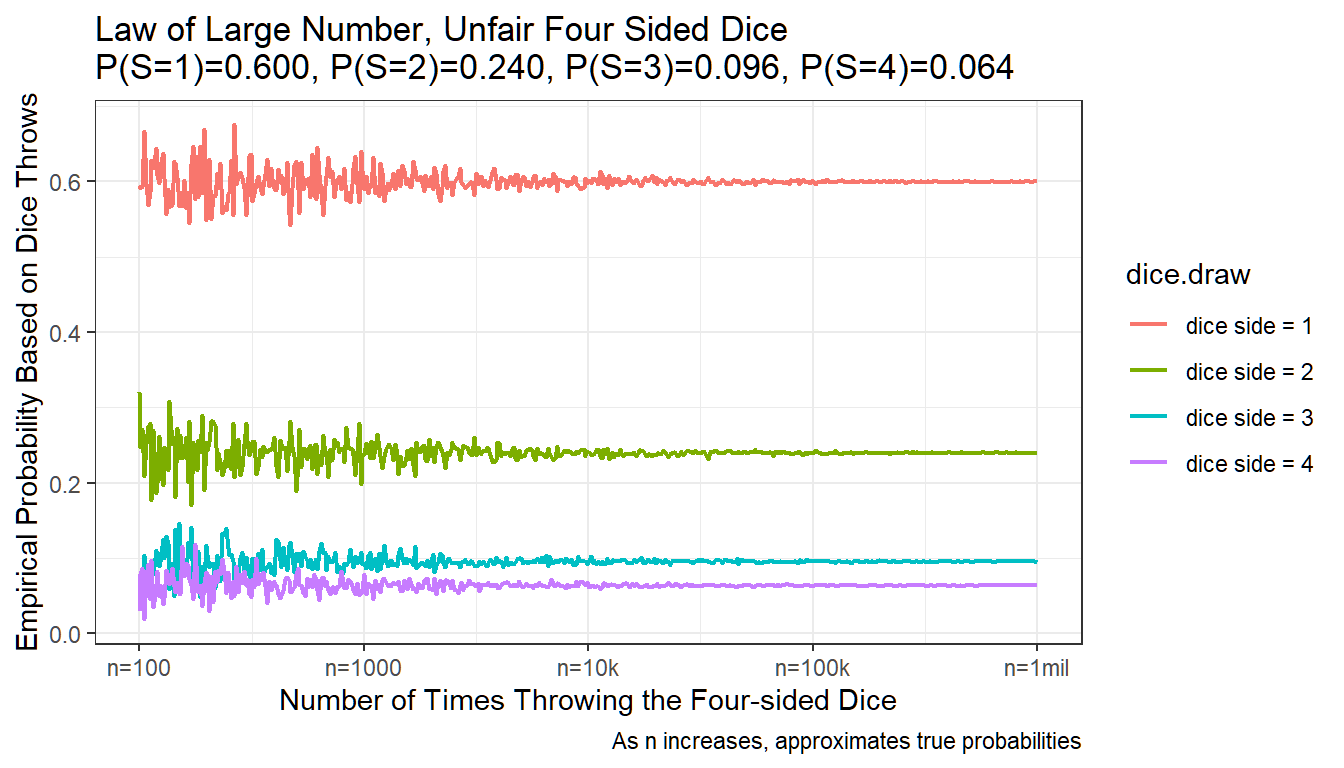
\includegraphics{Introductory-Statistics-with-R-tidyverse_files/figure-latex/unnamed-chunk-67-1} \end{center}

\hypertarget{multiple-step-experiment}{%
\section{Multiple-Step Experiment}\label{multiple-step-experiment}}

\begin{quote}
Go back to \href{http://fanwangecon.github.io/}{fan}'s \href{https://fanwangecon.github.io/REconTools/}{REconTools} Package, \href{https://fanwangecon.github.io/R4Econ/}{R Code Examples} Repository (\href{https://fanwangecon.github.io/R4Econ/bookdown}{bookdown site}), or \href{https://fanwangecon.github.io/Stat4Econ/}{Intro Stats with R} Repository (\href{https://fanwangecon.github.io/Stat4Econ/bookdown}{bookdown site}).
\end{quote}

\hypertarget{playing-the-lottery-three-times}{%
\subsection{Playing the Lottery Three times}\label{playing-the-lottery-three-times}}

In \emph{\href{https://fanwangecon.github.io/Stat4Econ/probability/htmlpdfr/samplespace.html}{Sample Space, Experimental Outcomes, Events, Probabilities}}, we discussed various definitions. We studied various examples in \href{https://fanwangecon.github.io/Stat4Econ/probability/htmlpdfr/samplespaceexa.html}{\emph{Examples of Sample Space and Probabilities}}.

In the example below, we have a multiple-step experiment: ``If an experiment can be describe as a sequence of \(n\) steps with \(m\) possible outcomes on each step, then the total number of experimental outcomes is \(m^n\).'' (ASWCC P172) You can use letters other than \(n\) and \(m\) as well.

Key questions:

\begin{itemize}
\tightlist
\item
  What are the possible experimental outcomes?
\item
  What are the probabilities associated with each of the experimental outcomes?
\end{itemize}

We are thinking about the problem from day zero perspective. We could play the lottery three times, on day one, day two and day three.

Suppose you can either win or lose when you play the lottery. Each lottery ticket costs the same. You will buy 1 lottery ticket on each day for three days straight. The chance of winning is the same for each lottery ticket (perhaps the number of people buying lottery is the same every day). You see at the end of each day whether you won or lost.

The question is, what are the possible outcomes after three days? You are standing from the perspective of today, looking forward to what could happen tomorrow, two days from now, three days from now.

\hypertarget{assumptions-and-symbols}{%
\subsubsection{Assumptions and Symbols}\label{assumptions-and-symbols}}

\emph{Assumptions}

Based on the descriptions above, we can write down the following assumptions we are making, which are also the assumptions for the binomial distribution:

\begin{enumerate}
\def\labelenumi{\arabic{enumi}.}
\tightlist
\item
  There are \(n\) numbers of identical lottery plays
\item
  The outcomes of each lottery are always win or lose, just these two possible outcomes.
\item
  The chance of winning each time, \(p_{\text{win}}\), is the same during each play. The chance of losing is the same as well, \(1-p_{\text{win}}\).
\item
  Whether you won or not before does not impact whether you will win in the future.
\end{enumerate}

\emph{Symbols we will use}

\begin{enumerate}
\def\labelenumi{\arabic{enumi}.}
\tightlist
\item
  \(n\): denotes the number of lottery plays (number of trials)
\item
  \(x\): denotes the number of times you win, at most \(x=n\), at least \(x=0\), the number of losses is \(n-x\)
\item
  \(p\): the probability of winning, the probability of losing is therefore \(1-p\).
\end{enumerate}

The Tree Structure with Probability Written on it, \emph{Notations}:

\begin{itemize}
\tightlist
\item
  W = Win, L = Lose
\item
  D0 = Day 0, D1 = Day 1, D2 = Day 2
\end{itemize}

\hypertarget{play-the-lottery-just-once}{%
\subsubsection{Play the Lottery Just once}\label{play-the-lottery-just-once}}

From day zero perspective, by the end of day one, there are two possible experimental outcomes, with different probabilities associated with each outcome.

\begin{itemize}
\tightlist
\item
  D0:

  \begin{itemize}
  \tightlist
  \item
    D1 \(W\): \(P(E_1) = P(W) = p\)
  \item
    D1 \(L\): \(P(E_2) = P(L) = 1-p\)
  \end{itemize}
\end{itemize}

There are two experimental outcomes in the sample space:
\[\Sigma_{i=1}^2 \left(P\left(E_i\right)\right) = p + \left(1-p\right) = 1\]

\hypertarget{play-the-lottery-twice}{%
\subsubsection{Play the Lottery Twice}\label{play-the-lottery-twice}}

From day zero perspective, by the end of day two, there are four possible experimental outcomes, with different probabilities associated with each outcome.

We are assuming that each lottery play is independent, we learned \href{https://fanwangecon.github.io/Stat4Econ/probability/htmlpdfr/samplespace.html}{before} that:

\[ P(A \cap B) = P (A \mid B)\cdot P(B)\]

and when \(A\) and \(B\) are independent:

\[ P(A \cap B) = P (A)\cdot P(B)\]

\begin{itemize}
\tightlist
\item
  D0:

  \begin{itemize}
  \tightlist
  \item
    D1 W:

    \begin{itemize}
    \tightlist
    \item
      D2 \(W\): \(P(E_1) = P(\text{First Game Win} \cap \text{Second Game Win}) = P(WW) = P(W) \cdot P(W) = p \cdot p\)
    \item
      D2 \(L\): \(P(E_2) = P(\text{First Game Win} \cap \text{Second Game Lose}) = P(WL) = P(W) \cdot \left(1-P(W)\right) = p \cdot (1-p)\)
    \end{itemize}
  \item
    D1 L:

    \begin{itemize}
    \tightlist
    \item
      D2 \(W\): \(P(E_3) = P(LW)=(1-p) \cdot p\)
    \item
      D2 \(L\): \(P(E_4) = P(LL)=(1-p) \cdot (1-p)\)
    \end{itemize}
  \end{itemize}
\end{itemize}

There are four experimental outcomes in the sample space:

\begin{align}
\Sigma_{i=1}^4 \left(P\left(E_i\right)\right) =& p \cdot p + p \cdot (1-p) + (1-p) \cdot p + (1-p) \cdot (1-p)\\
=& p \cdot (p + 1 - p) + (1-p) \cdot (p + 1 - p) \\
=& p + (1-p) \\
=& 1 \\
\end{align}

\hypertarget{play-the-lottery-three-times}{%
\subsubsection{Play the Lottery Three Times}\label{play-the-lottery-three-times}}

From day zero perspective, by the end of day three, there are eight possible experimental outcomes, with different probabilities associated with each outcome.

\begin{itemize}
\tightlist
\item
  D0:

  \begin{itemize}
  \tightlist
  \item
    D1 \(W\):

    \begin{itemize}
    \tightlist
    \item
      D2 \(W\)

      \begin{itemize}
      \tightlist
      \item
        D3 \(W\): \(P(E_1)=P(WWW)=p^{3} \cdot (1-p)^{0}\)
      \item
        D3 \(L\): \(P(E_2)=P(WWL)=p^{2} \cdot (1-p)^{1}\)
      \end{itemize}
    \item
      D2 \(L\):

      \begin{itemize}
      \tightlist
      \item
        D3 \(W\): \(P(E_3)=P(WLW)=p^{2} \cdot (1-p)^{1}\)
      \item
        D3 \(L\): \(P(E_4)=P(WLL)=p^{1} \cdot (1-p)^{2}\)
      \end{itemize}
    \end{itemize}
  \item
    D1 \(L\):

    \begin{itemize}
    \tightlist
    \item
      D2 \(W\)

      \begin{itemize}
      \tightlist
      \item
        D3 \(W\): \(P(E_5)=P(LWW)=p^{2} \cdot (1-p)^{1}\)
      \item
        D3 \(L\): \(P(E_6)=P(LWL)=p^{1} \cdot (1-p)^{2}\)
      \end{itemize}
    \item
      D2 \(L\):

      \begin{itemize}
      \tightlist
      \item
        D3 \(W\): \(P(E_7)=P(LLW)=p^{1} \cdot (1-p)^{2}\)
      \item
        D3 \(L\): \(P(E_8)=P(LLL)=p^{0} \cdot (1-p)^{3}\)
      \end{itemize}
    \end{itemize}
  \end{itemize}
\end{itemize}

There are eight experimental outcomes in the sample space, and they sum up to one as before:

\begin{align}
\Sigma_{i=1}^8 \left(P\left(E_i\right)\right) = 1 \\
\end{align}

\hypertarget{probabilities-of-events}{%
\subsubsection{Probabilities of Events}\label{probabilities-of-events}}

Generally, after \(n\) trials/lotteries, if a particular experimental outcome had \(x\) number of wins/successes (which means \(n-x\) number of losses/failures), the probability that this particular experimental outcome happen is:
\[ p^x \cdot p^{n-x} \]

The probabilities we wrote in the previous examples all follow this rule. Remember that if someone won every time, \(n=x\), and we will have \(p^x \cdot p^{n-x}=p^x \cdot p^0 = p^x \cdot 1 = p^x\).

So far we have discussed different experimental outcomes with unique sequences of wins and losses. In the 3 lottery example above, we have 8 experimental outcomes. If we are mainly interested in the total number of wins and losses, we can group these 8 experimental outcomes into 4 events.

\begin{enumerate}
\def\labelenumi{\arabic{enumi}.}
\tightlist
\item
  Event win three times: W3 = \(\left\{E_1\right\}\)
  \[P(W3)=p^{3} \cdot (1-p)^{0}\]
\item
  Event win two times: W2 = \(\left\{E_2, E_3, E_5\right\}\)

  \begin{itemize}
  \tightlist
  \item
    There are three experimental outcomes out of the eight where you win two times. The probability of each of these experimental outcomes happening is: \(p^{2} \cdot (1-p)^{1}\), hence: \[P(W2) = 3 \cdot p^{2} \cdot (1-p)^{1}\]
  \end{itemize}
\item
  Event win one time: W1 = \(\left\{E_4, E_6, E_7\right\}\)

  \begin{itemize}
  \tightlist
  \item
    There are three experimental outcomes out of the eight where you win one time. The probability of each of these experimental outcomes happening is: \(p^{1} \cdot (1-p)^{2}\), hence: \[P(W1) = 3 \cdot p^{1} \cdot (1-p)^{2}\]
  \end{itemize}
\item
  Event win zero time: W0 = \(\left\{E_8\right\}\)
  \[P(W0)=p^{0} \cdot (1-p)^{3}\]
\end{enumerate}

These four events are \href{https://fanwangecon.github.io/Stat4Econ/probability/htmlpdfr/samplespace.html}{mutually exclusive and jointly exhaustive}, we can define a new sample space that includes four experimental outcomes, win zero times, win once, win twice, win three times.

\hypertarget{discrete-probability-distribution}{%
\chapter{Discrete Probability Distribution}\label{discrete-probability-distribution}}

\hypertarget{discrete-random-variable-and-binomial}{%
\section{Discrete Random Variable and Binomial}\label{discrete-random-variable-and-binomial}}

\begin{quote}
Go back to \href{http://fanwangecon.github.io/}{fan}'s \href{https://fanwangecon.github.io/REconTools/}{REconTools} Package, \href{https://fanwangecon.github.io/R4Econ/}{R Code Examples} Repository (\href{https://fanwangecon.github.io/R4Econ/bookdown}{bookdown site}), or \href{https://fanwangecon.github.io/Stat4Econ/}{Intro Stats with R} Repository (\href{https://fanwangecon.github.io/Stat4Econ/bookdown}{bookdown site}).
\end{quote}

We have been looking at various examples of discrete Random Variables in \href{https://fanwangecon.github.io/Stat4Econ/probability/htmlpdfr/samplespace.html}{Sample Space, Experimental Outcomes, Events, Probabilities}, \href{https://fanwangecon.github.io/Stat4Econ/probability/htmlpdfr/samplespaceexa.html}{Examples of Sample Space and Probabilities}, \href{https://fanwangecon.github.io/Stat4Econ/probability/htmlpdfr/lottery.html}{Multiple-Step Experiment: Playing the Lottery Three times}, and \href{https://fanwangecon.github.io/Stat4Econ/probability/htmlpdfr/samplespacedice.html}{Throw an Unfair Four Sided Dice}.

Now we state this a little bit more formally.

\hypertarget{discrete-random-variable}{%
\subsection{Discrete Random Variable}\label{discrete-random-variable}}

\begin{enumerate}
\def\labelenumi{\arabic{enumi}.}
\tightlist
\item
  Random Variable

  \begin{itemize}
  \tightlist
  \item
    ``A random variable is a numerical description of the outcome of an experiment.'' (ASWCC P217)
    \[ \text{we could use letter } x \text{ to represent a random variable}\]
  \end{itemize}
\item
  Discrete Random Variables

  \begin{itemize}
  \tightlist
  \item
    ``A random variable that may assume either a finite number of values or an infinite sequence of values such as \(0,1,2,...\) is referred to as a discrete random variable.'' (ASWCC P217)
  \end{itemize}
\item
  Discrete Probability Mass Function

  \begin{itemize}
  \tightlist
  \item
    ``For a discrete random variable \(x\), a probability function, denoted by \(f(x)\), provides the probability for each value of the random variable.'' (ASWCC P220)
  \item
    We can think of different values of \(x\) as been mapped from an experimental outcome in the sample space. Probability can not be negative, and the sum of the probability of different possible \(x\) outcomes sum to 1 (ASWCC P221):
    \[ f(x) \ge 0\]
    \[\Sigma f(x) = 1\]
  \end{itemize}
\item
  Expected Value of a Discrete Random Variable (ASWCC P225)
  \[E(x) = \mu_x = \Sigma x \cdot f(x)\]
\item
  Variance of a Discrete Random Variable (ASWCC P225)
  \[Var(x) = \sigma_x^2 = \Sigma \left( (x - \mu_x)^2 \cdot f(x) \right)\]
\end{enumerate}

\emph{Well Known Discrete Probability Distributions}

There is a \href{https://en.wikipedia.org/wiki/List_of_probability_distributions\#Discrete_distributions}{variety of} different Discrete Random Variable Probability Mass Functions that are appropriate for analyzing different situations. Think of these as tools, you don't need to memorize the formulas, but you can learn about under what conditions these distributions are useful. Learn about the parameters of these distributions, and use the appropriate Excel or R function.

The simplest distribution is the \href{https://en.wikipedia.org/wiki/Discrete_uniform_distribution}{Discrete Uniform Distribution}. The uniform probability mass function is: \(f(x) = \frac{1}{n}\), where \(n\) is the \emph{the number of values the random variable may assume}, corresponding to experimental outcomes. (ASWCC P222)

We focus on the Binomial Distribution here, a variety of other distributions are related to the binomial distribution:

\begin{itemize}
\tightlist
\item
  \href{https://en.wikipedia.org/wiki/Binomial_distribution}{Binomial Distribution}
\item
  \href{https://en.wikipedia.org/wiki/Bernoulli_distribution}{Bernoulli Distribution}
\item
  \href{https://en.wikipedia.org/wiki/Hypergeometric_distribution}{Hypergeometric Distribution}
\item
  \href{https://en.wikipedia.org/wiki/Beta-binomial_distribution}{Beta-Binomial Distribution}
\end{itemize}

\hypertarget{binomial-experiment}{%
\section{Binomial Experiment}\label{binomial-experiment}}

We have already examined \href{https://fanwangecon.github.io/Stat4Econ/probability/htmlpdfr/lottery.html}{Multiple-Step Experiment: Playing the Lottery Three times}. Here we re-state the four properties of the \href{https://en.wikipedia.org/wiki/Binomial_distribution}{Binomial Experiment} (ASWCC P240):

\begin{enumerate}
\def\labelenumi{\arabic{enumi}.}
\tightlist
\item
  ``The experiment consists of a sequence of \(n\) identical trials.''
\item
  ``Two outcomes are possible on each trial. We refer to one outcome as a success and the other outcome as a failure.''
\item
  ``The probability of a success, denoted by \(p\), does not change from trial to trial. Consequently, the probability of a failure, denoted by \(1-p\), does not change from trial to trial.''
\item
  ``The trials are independent.''
\end{enumerate}

\textbf{Binomial Sample Space}

Note that given that there are \(n\) trials, the possible \(x\) go from \(x=0\) to \(x=n\). In another word, if there are three trials, \(n=3\), there are four possible experimental outcomes for \(x\).

\begin{itemize}
\tightlist
\item
  Experiment: The binomial experiment with \(n\) trials
\item
  Experimental outcomes: \(x=0,x=1,...,x=\left(n-1\right),x=n\)
\item
  Sample Space: \(S=\left\{0,1,...,n-1,n\right\}\)
\end{itemize}

\textbf{Binomial Probability Mass Funcion}

What is the probability of having \(x\) success out of \(n\) trials, given that there is \(p\) chance of success for each trial and the assumptions above? The answer is given by this formula, which is the binomial probability mass function:
\[
f(x;n,p) = C^{n}_{x} \cdot p^x \cdot \left(1-p\right)^{n-x}
         = \frac{n!}{\left(n-x\right)! \cdot x!} \cdot p^x \cdot \left(1-p\right)^{n-x}\\
\]

With the binomial experiment, we can now use a formula to assign probabilities. A formula is a piece of machinery that takes inputs and spits out outputs, Thie binomial probability mass function has three inputs, \(x\), \(n\) and \(p\). You need to tell R, Excel, or alternative programs what these three numbers are, and the program will spit a probability out for you. \(n\) and \(p\) are the parameters.

\textbf{Binomial Expected Value and Variance}

For the binomial discrete random variable, it turns out the expected value and variance are:
\[E(x) = n \cdot p\]
\[Var(x) = n \cdot p \cdot (1-p)\]
We can find the expected value and variance by summing over all terms following: \(E(x) = \mu_x = \Sigma x \cdot f(x)\) and \(Var(x) = \sigma_x^2 = \Sigma \left( (x - \mu_x)^2 \cdot f(x) \right)\), and we will always end up with these two results. It is intuitive. The average number of wins given that you play \(n\) trials and given that the chance of winning each game is \(p\) is \(n \cdot p\).

\hypertarget{binomial-example-larceny}{%
\subsection{Binomial Example: Larceny}\label{binomial-example-larceny}}

In 2004, in the United State, \href{https://en.wikipedia.org/wiki/Clearance_rate}{18.3 percent of Larceny-Theft were cleared}. ``Clearance rates are used by various groups as a measure of crimes solved by the police.''

\hypertarget{chance-of-x-out-n-arrested}{%
\subsubsection{Chance of x out n Arrested}\label{chance-of-x-out-n-arrested}}

10 people commit 10 larceny-theft crimes, suppose the situation follows the conditions of the binomial experiment, what is the chance that nobody is arrested? The chance that 1, 2, 3, or all 10 are arrested?

\begin{itemize}
\tightlist
\item
  \(n=10\): 10 crimes, 10 trials
\item
  \(p=0.183\): what is \(p\) here? For the police success is clearing a crime.
\item
  \(x\): if \(x=10\), that means all larceny-thefts were cleared, if \(x=0\), this means the police failed to clear all 10 thefts.
\end{itemize}

For example, the chance that \(2\) out of \(10\) is arrested is:
\[f\left(x=2;n=10,p=0.183\right) = \frac{10!}{\left(10-2\right)! \cdot 2!} \cdot 0.183^2 \cdot \left(1-0.183\right)^{10-2} = 0.299\]

We can use the r function, \emph{dbinom}, to calculate these probabilites: \emph{dbinom(2,10,0.183)}. Additionally, \emph{pbinom(2,10,0.183)} tells us the cumulative probability that at most 2 out of 10 are arrested.

We do this in the code below. From the graph below, we can see that there is a 13.3\% chance that none of the 10 thieves would be arrested, and alomst 0 percent chance that all 10 of then would be arrested. The chance that 6 out of the 10 thiefs would be arrested is less than 1 percent.

\begin{Shaded}
\begin{Highlighting}[]
\CommentTok{\# library}
\KeywordTok{library}\NormalTok{(tidyverse)}

\CommentTok{\# Parameters}
\NormalTok{n \textless{}{-}}\StringTok{ }\DecValTok{10}
\NormalTok{p \textless{}{-}}\StringTok{ }\FloatTok{0.183}

\CommentTok{\# A vector of different arrest counts}
\NormalTok{zero2max \textless{}{-}}\StringTok{ }\DecValTok{0}\OperatorTok{:}\NormalTok{n}

\CommentTok{\# Probability for different arrest counts}
\NormalTok{prob\_of\_arrests \textless{}{-}}\StringTok{ }\KeywordTok{dbinom}\NormalTok{(zero2max, n, p)}

\CommentTok{\# Control Graph Size}
\KeywordTok{options}\NormalTok{(}\DataTypeTok{repr.plot.width =} \DecValTok{5}\NormalTok{, }\DataTypeTok{repr.plot.height =} \DecValTok{4}\NormalTok{)}

\CommentTok{\# Number of Arrests Probabilities}
\NormalTok{arrest.prob.mass \textless{}{-}}\StringTok{ }\KeywordTok{tibble}\NormalTok{(}\DataTypeTok{arrests=}\NormalTok{zero2max, }\DataTypeTok{prob=}\NormalTok{prob\_of\_arrests)}

\CommentTok{\# Titles Strings etc}
\NormalTok{graph.title \textless{}{-}}\StringTok{ }\KeywordTok{sprintf}\NormalTok{(}\StringTok{\textquotesingle{}Prob for Number of Theft{-}Criminals Arrested out of \%s\textquotesingle{}}\NormalTok{ ,n)}
\NormalTok{graph.caption \textless{}{-}}\StringTok{ }\KeywordTok{sprintf}\NormalTok{(}
    \KeywordTok{paste0}\NormalTok{(}\StringTok{\textquotesingle{}Assuming the binomial properties apply}\CharTok{\textbackslash{}n}\StringTok{\textquotesingle{}}\NormalTok{,}
           \StringTok{\textquotesingle{}2004 Larceny/Left USA Clearance Rate = \%s\textquotesingle{}}\NormalTok{), p)}

\CommentTok{\# Create a Table and Graph it}
\NormalTok{arrest.graph \textless{}{-}}\StringTok{ }\NormalTok{arrest.prob.mass }\OperatorTok{\%\textgreater{}\%}
\StringTok{    }\KeywordTok{ggplot}\NormalTok{(}\KeywordTok{aes}\NormalTok{(}\DataTypeTok{x=}\NormalTok{arrests, }\DataTypeTok{y=}\NormalTok{prob, }\DataTypeTok{label =} \KeywordTok{sprintf}\NormalTok{(}\StringTok{\textquotesingle{}\%0.3f\textquotesingle{}}\NormalTok{, prob))) }\OperatorTok{+}
\StringTok{    }\KeywordTok{geom\_bar}\NormalTok{(}\DataTypeTok{stat =} \StringTok{\textquotesingle{}identity\textquotesingle{}}\NormalTok{) }\OperatorTok{+}
\StringTok{    }\KeywordTok{geom\_text}\NormalTok{(}\DataTypeTok{vjust =} \FloatTok{{-}0.5}\NormalTok{, }\DataTypeTok{size =} \DecValTok{3}\NormalTok{) }\OperatorTok{+}
\StringTok{    }\KeywordTok{labs}\NormalTok{(}\DataTypeTok{title =}\NormalTok{ graph.title,}
         \DataTypeTok{x =} \StringTok{\textquotesingle{}Number of Criminals Arrests\textquotesingle{}}\NormalTok{,}
         \DataTypeTok{y =} \StringTok{\textquotesingle{}Prob of x Arrested\textquotesingle{}}\NormalTok{,}
         \DataTypeTok{caption =}\NormalTok{ graph.caption) }\OperatorTok{+}
\StringTok{    }\KeywordTok{scale\_x\_continuous}\NormalTok{(}\DataTypeTok{labels =}\NormalTok{ zero2max, }\DataTypeTok{breaks =}\NormalTok{ zero2max) }\OperatorTok{+}
\StringTok{    }\KeywordTok{theme\_bw}\NormalTok{()}

\KeywordTok{print}\NormalTok{(arrest.graph)}
\end{Highlighting}
\end{Shaded}

\begin{center}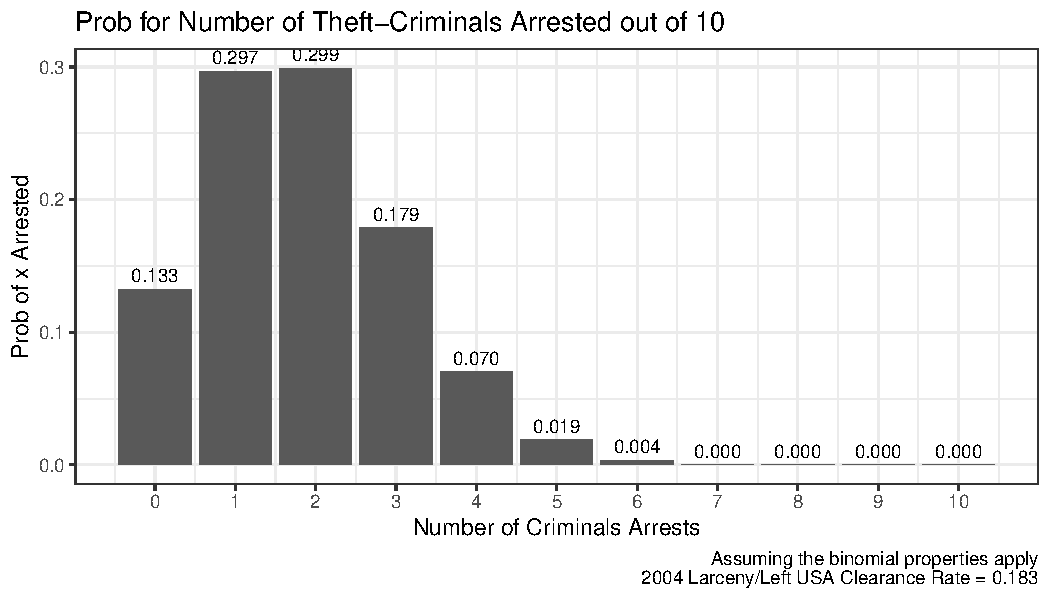
\includegraphics{Introductory-Statistics-with-R-tidyverse_files/figure-latex/unnamed-chunk-70-1} \end{center}

\hypertarget{what-is-the-chance-of-arrest-at-least-x-out-of-n-people}{%
\subsubsection{What is the Chance of Arrest at Least X out of N People}\label{what-is-the-chance-of-arrest-at-least-x-out-of-n-people}}

What is the chance that at most 3 out of the 10 thiefs are arrested? That includes the chance that no one is arrested, 1, 2, or 3 people are arrested:

\[
 p\left(x \le 3;n=10,p=0.183\right) \\
=\Sigma_{x=0}^{3} \left( f\left(x;n=10,p=0.183\right) \right) \\
=\Sigma_{x=0}^3 \left( \frac{10!}{\left(10-x\right)! \cdot x!} \cdot 0.183^x \cdot \left(1-0.183\right)^{10-x} \right)\\
=0.133 + 0.297 + 0.299 + 0.179\\
=0.907\\
\]

Given the low clearance rate, there is a \(90\) percent chance that at most 3 out of 10 criminals are arrested.

We can graph this out. We will graph the previous graph again but overlay the cumulative probability on top.

\begin{Shaded}
\begin{Highlighting}[]
\CommentTok{\# Cumulative Probability for different arrest counts, before dbinom, now pbinom}
\NormalTok{cumulative\_prob\_of\_arrests \textless{}{-}}\StringTok{ }\KeywordTok{pbinom}\NormalTok{(zero2max, n, p)}

\CommentTok{\# Data File that Includes Cumulative Probability and Mass}
\NormalTok{arrest.prob \textless{}{-}}\StringTok{ }\KeywordTok{tibble}\NormalTok{(}\DataTypeTok{arrests=}\NormalTok{(zero2max), }\DataTypeTok{prob=}\NormalTok{prob\_of\_arrests, }\DataTypeTok{cum.prob=}\NormalTok{cumulative\_prob\_of\_arrests)}

\CommentTok{\# Control Graph Size}
\KeywordTok{options}\NormalTok{(}\DataTypeTok{repr.plot.width =} \DecValTok{5}\NormalTok{, }\DataTypeTok{repr.plot.height =} \DecValTok{4}\NormalTok{)}

\CommentTok{\# Create a Table and Graph it}
\CommentTok{\#     geom\_text(aes(y=prob, label = sprintf(\textquotesingle{}\%0.3f\textquotesingle{}, prob)), vjust = {-}0.5, size = 3) +}

\NormalTok{axis.sec.ratio \textless{}{-}}\StringTok{ }\KeywordTok{max}\NormalTok{(cumulative\_prob\_of\_arrests)}\OperatorTok{/}\KeywordTok{max}\NormalTok{(prob\_of\_arrests)}
\NormalTok{right.axis.color \textless{}{-}}\StringTok{ \textquotesingle{}blue\textquotesingle{}}
\NormalTok{left.axis.color \textless{}{-}}\StringTok{ \textquotesingle{}red\textquotesingle{}}

\CommentTok{\# Probabilities}
\NormalTok{arrest.graph \textless{}{-}}\StringTok{ }\NormalTok{arrest.prob }\OperatorTok{\%\textgreater{}\%}
\StringTok{    }\KeywordTok{ggplot}\NormalTok{(}\KeywordTok{aes}\NormalTok{(}\DataTypeTok{x=}\NormalTok{arrests)) }\OperatorTok{+}
\StringTok{    }\KeywordTok{geom\_bar}\NormalTok{(}\KeywordTok{aes}\NormalTok{(}\DataTypeTok{y=}\NormalTok{prob),}
             \DataTypeTok{stat=}\StringTok{\textquotesingle{}identity\textquotesingle{}}\NormalTok{, }\DataTypeTok{alpha=}\FloatTok{0.5}\NormalTok{, }\DataTypeTok{width=}\FloatTok{0.5}\NormalTok{, }\DataTypeTok{fill=}\NormalTok{left.axis.color) }\OperatorTok{+}
\StringTok{    }\KeywordTok{geom\_text}\NormalTok{(}\KeywordTok{aes}\NormalTok{(}\DataTypeTok{y=}\NormalTok{prob,}
                  \DataTypeTok{label =} \KeywordTok{paste0}\NormalTok{(}\KeywordTok{sprintf}\NormalTok{(}\StringTok{\textquotesingle{}\%2.1f\textquotesingle{}}\NormalTok{, prob}\OperatorTok{*}\DecValTok{100}\NormalTok{), }\StringTok{\textquotesingle{}\%\textquotesingle{}}\NormalTok{)),}
              \DataTypeTok{vjust =} \FloatTok{{-}0.5}\NormalTok{, }\DataTypeTok{size =} \DecValTok{3}\NormalTok{, }\DataTypeTok{color=}\NormalTok{left.axis.color, }\DataTypeTok{fontface=}\StringTok{\textquotesingle{}bold\textquotesingle{}}\NormalTok{)}

\CommentTok{\# Cumulative Probabilities}
\NormalTok{arrest.graph \textless{}{-}}\StringTok{ }\NormalTok{arrest.graph }\OperatorTok{+}
\StringTok{    }\KeywordTok{geom\_line}\NormalTok{(}\KeywordTok{aes}\NormalTok{(}\DataTypeTok{y=}\NormalTok{cum.prob}\OperatorTok{/}\NormalTok{axis.sec.ratio),}
              \DataTypeTok{alpha=}\FloatTok{0.25}\NormalTok{, }\DataTypeTok{size=}\DecValTok{1}\NormalTok{, }\DataTypeTok{color=}\NormalTok{right.axis.color) }\OperatorTok{+}
\StringTok{    }\KeywordTok{geom\_point}\NormalTok{(}\KeywordTok{aes}\NormalTok{(}\DataTypeTok{y=}\NormalTok{cum.prob}\OperatorTok{/}\NormalTok{axis.sec.ratio),}
               \DataTypeTok{alpha=}\FloatTok{0.75}\NormalTok{, }\DataTypeTok{size=}\DecValTok{2}\NormalTok{, }\DataTypeTok{shape=}\DecValTok{23}\NormalTok{, }\DataTypeTok{fill=}\NormalTok{right.axis.color) }\OperatorTok{+}
\StringTok{    }\KeywordTok{geom\_text}\NormalTok{(}\KeywordTok{aes}\NormalTok{(}\DataTypeTok{y=}\NormalTok{cum.prob}\OperatorTok{/}\NormalTok{axis.sec.ratio,}
                  \DataTypeTok{label =} \KeywordTok{paste0}\NormalTok{(}\KeywordTok{sprintf}\NormalTok{(}\StringTok{\textquotesingle{}\%2.0f\textquotesingle{}}\NormalTok{, cum.prob}\OperatorTok{*}\DecValTok{100}\NormalTok{), }\StringTok{\textquotesingle{}\%\textquotesingle{}}\NormalTok{)),}
              \DataTypeTok{vjust =} \FloatTok{{-}0.5}\NormalTok{, }\DataTypeTok{size =} \DecValTok{3}\NormalTok{, }\DataTypeTok{color=}\NormalTok{right.axis.color, }\DataTypeTok{fontface=}\StringTok{\textquotesingle{}bold\textquotesingle{}}\NormalTok{)}

\CommentTok{\# Titles Strings etc}
\NormalTok{graph.title \textless{}{-}}\StringTok{ }\KeywordTok{sprintf}\NormalTok{(}
    \KeywordTok{paste0}\NormalTok{(}\StringTok{\textquotesingle{}Number of Theft{-}Criminals Arrested out of \%s}\CharTok{\textbackslash{}n}\StringTok{\textquotesingle{}}\NormalTok{,}
           \StringTok{\textquotesingle{}Prob Mass (Left) and Cumulative Prob (Right)\textquotesingle{}}\NormalTok{), n)}
\NormalTok{graph.caption \textless{}{-}}\StringTok{ }\KeywordTok{sprintf}\NormalTok{(}
    \KeywordTok{paste0}\NormalTok{(}\StringTok{\textquotesingle{}Assuming the binomial properties apply}\CharTok{\textbackslash{}n}\StringTok{\textquotesingle{}}\NormalTok{,}
           \StringTok{\textquotesingle{}2004 Larceny/Left USA Clearance Rate = \%s\textquotesingle{}}\NormalTok{), p)}
\NormalTok{graph.title.x \textless{}{-}}\StringTok{ \textquotesingle{}Number of Criminals Arrests\textquotesingle{}}
\NormalTok{graph.title.y.axisleft \textless{}{-}}\StringTok{ \textquotesingle{}Prob of x Arrested\textquotesingle{}}
\NormalTok{graph.title.y.axisright \textless{}{-}}\StringTok{ \textquotesingle{}Prob of at most x Arrested\textquotesingle{}}

\CommentTok{\# Title}
\NormalTok{arrest.graph \textless{}{-}}\StringTok{ }\NormalTok{arrest.graph }\OperatorTok{+}
\StringTok{    }\KeywordTok{labs}\NormalTok{(}\DataTypeTok{title =}\NormalTok{ graph.title,}
         \DataTypeTok{x =}\NormalTok{ graph.title.x, }\DataTypeTok{y =}\NormalTok{ graph.title.y.axisleft,}
         \DataTypeTok{caption =}\NormalTok{ graph.caption) }\OperatorTok{+}
\StringTok{    }\KeywordTok{scale\_y\_continuous}\NormalTok{(}\DataTypeTok{sec.axis =}
                       \KeywordTok{sec\_axis}\NormalTok{(}\OperatorTok{\textasciitilde{}}\NormalTok{.}\OperatorTok{*}\NormalTok{axis.sec.ratio, }\DataTypeTok{name =}\NormalTok{ graph.title.y.axisright)) }\OperatorTok{+}
\StringTok{    }\KeywordTok{scale\_x\_continuous}\NormalTok{(}\DataTypeTok{labels =}\NormalTok{ zero2max, }\DataTypeTok{breaks =}\NormalTok{ zero2max) }\OperatorTok{+}
\StringTok{    }\KeywordTok{theme}\NormalTok{(}\DataTypeTok{axis.text.y =} \KeywordTok{element\_text}\NormalTok{(}\DataTypeTok{face=}\StringTok{\textquotesingle{}bold\textquotesingle{}}\NormalTok{),}
          \DataTypeTok{axis.text.y.right =} \KeywordTok{element\_text}\NormalTok{(}\DataTypeTok{color =}\NormalTok{ right.axis.color),}
          \DataTypeTok{axis.text.y.left =} \KeywordTok{element\_text}\NormalTok{(}\DataTypeTok{color =}\NormalTok{ left.axis.color))}

\CommentTok{\# Print}
\KeywordTok{print}\NormalTok{(arrest.graph)}
\end{Highlighting}
\end{Shaded}

\begin{center}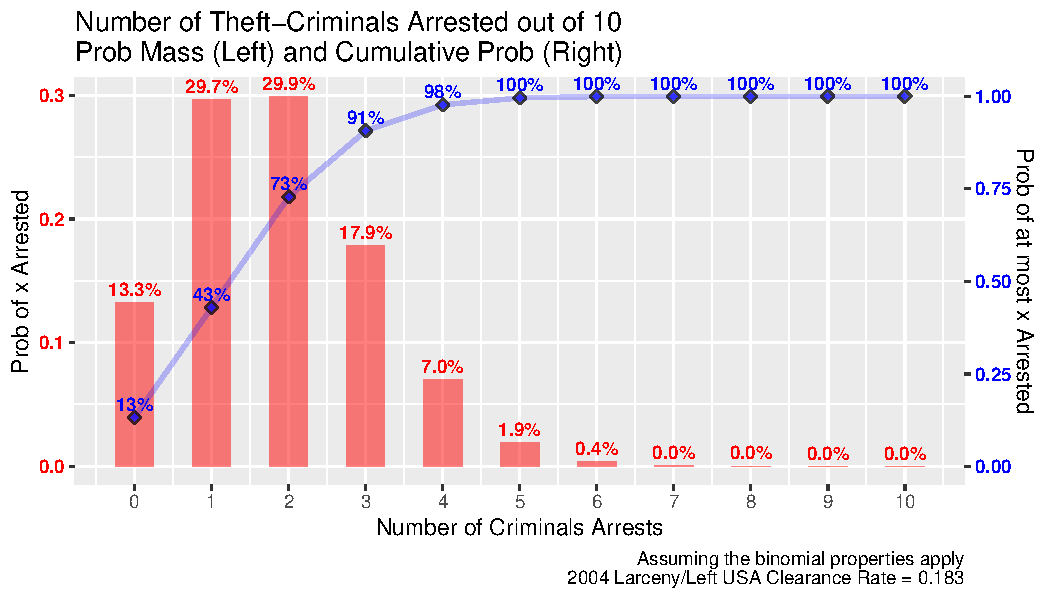
\includegraphics{Introductory-Statistics-with-R-tidyverse_files/figure-latex/unnamed-chunk-71-1} \end{center}

\hypertarget{binomial-example-wwii-german-soldier}{%
\subsection{Binomial Example: WWII German Soldier}\label{binomial-example-wwii-german-soldier}}

During WWII, 13.6 million Germans served in the German army, and 4.2 million were killed or missing. This is a death rate of \href{https://en.wikipedia.org/wiki/World_War_II_casualties\#Military_casualties_by_branch_of_service}{30.9 percent}.

Suppose there are many German towns that each sent 100 soldiers to the front, suppose the binomial properties apply, what is the fraction of solidiers who will return to their towns after the war?

\begin{itemize}
\tightlist
\item
  \(n=100\): suppose 100 solidiers from each German town went to join the German Army during WWII.
\item
  \(p=1-0.309=0.691\): \(p\) is the chance of survival.
\item
  \(x\): if \(x=1\), that means 1 out of 100 survived.
\end{itemize}

\begin{Shaded}
\begin{Highlighting}[]
\CommentTok{\# Parameters}
\NormalTok{n \textless{}{-}}\StringTok{ }\DecValTok{100}
\NormalTok{p \textless{}{-}}\StringTok{ }\DecValTok{1}\FloatTok{{-}0.309}

\CommentTok{\# Generate Data}
\CommentTok{\# A vector of different survival counts}
\NormalTok{zero2max \textless{}{-}}\StringTok{ }\DecValTok{0}\OperatorTok{:}\NormalTok{n}
\CommentTok{\# Probability for different survival counts}
\NormalTok{prob\_of\_survives \textless{}{-}}\StringTok{ }\KeywordTok{dbinom}\NormalTok{(zero2max, n, p)}
\CommentTok{\# Cumulative Probability for different survival counts, before dbinom, now pbinom}
\NormalTok{cumulative\_prob\_of\_survives \textless{}{-}}\StringTok{ }\KeywordTok{pbinom}\NormalTok{(zero2max, n, p)}
\CommentTok{\# Data File that Includes Cumulative Probability and Mass}
\NormalTok{survive.prob \textless{}{-}}\StringTok{ }\KeywordTok{tibble}\NormalTok{(}\DataTypeTok{survives=}\NormalTok{(zero2max), }\DataTypeTok{prob=}\NormalTok{prob\_of\_survives, }\DataTypeTok{cum.prob=}\NormalTok{cumulative\_prob\_of\_survives)}
\end{Highlighting}
\end{Shaded}

\hypertarget{wwii-german-soldiergraph}{%
\subsubsection{WWII German Soldier--Graph}\label{wwii-german-soldiergraph}}

We can see the results graphically as well below. Note that the graph looks normal. This is indeed the case, when \(n\) gets larger, the bionomial distribution approximates the normal distribution, with mean \(n\cdot p\) and variance \(n \cdot p \cdot (1-p)\).

Again this is given binomial assumptions. Which means in this case that soldiers from each town has equal probability of dying. And the chance of one soldier from a town dying does not change the chance of other soldiers from the same town dying. These are unlikely to be correct assumptions, but maybe they are approximately right.

We can see from the figure below that if the survival distribution follows binomial, less than 1 percent of towns should expect more than 80 out of 100 soldiers to return. And less than 1 percent of towns should expect less than 57 soldiers to return. Hence:

\begin{itemize}
\tightlist
\item
  Given a 30.9 percent death rate, nearly all German towns will have between 57 to 80 soldiers returning from the war out the 100 they sent to join the German army.
\end{itemize}

\begin{Shaded}
\begin{Highlighting}[]
\CommentTok{\# Control Graph Size}
\KeywordTok{options}\NormalTok{(}\DataTypeTok{repr.plot.width =} \DecValTok{5}\NormalTok{, }\DataTypeTok{repr.plot.height =} \DecValTok{4}\NormalTok{)}
\CommentTok{\# Two axis colors}
\NormalTok{axis.sec.ratio \textless{}{-}}\StringTok{ }\KeywordTok{max}\NormalTok{(cumulative\_prob\_of\_survives)}\OperatorTok{/}\KeywordTok{max}\NormalTok{(prob\_of\_survives)}
\NormalTok{right.axis.color \textless{}{-}}\StringTok{ \textquotesingle{}blue\textquotesingle{}}
\NormalTok{left.axis.color \textless{}{-}}\StringTok{ \textquotesingle{}red\textquotesingle{}}

\CommentTok{\# Probabilities}
\NormalTok{survive.graph \textless{}{-}}\StringTok{ }\NormalTok{survive.prob }\OperatorTok{\%\textgreater{}\%}
\StringTok{    }\KeywordTok{ggplot}\NormalTok{(}\KeywordTok{aes}\NormalTok{(}\DataTypeTok{x=}\NormalTok{survives)) }\OperatorTok{+}
\StringTok{    }\KeywordTok{geom\_bar}\NormalTok{(}\KeywordTok{aes}\NormalTok{(}\DataTypeTok{y=}\NormalTok{prob),}
             \DataTypeTok{stat=}\StringTok{\textquotesingle{}identity\textquotesingle{}}\NormalTok{, }\DataTypeTok{alpha=}\FloatTok{0.5}\NormalTok{, }\DataTypeTok{width=}\FloatTok{0.5}\NormalTok{, }\DataTypeTok{fill=}\NormalTok{left.axis.color)}

\CommentTok{\# Cumulative Probabilities}
\NormalTok{survive.graph \textless{}{-}}\StringTok{ }\NormalTok{survive.graph }\OperatorTok{+}
\StringTok{    }\KeywordTok{geom\_line}\NormalTok{(}\KeywordTok{aes}\NormalTok{(}\DataTypeTok{y=}\NormalTok{cum.prob}\OperatorTok{/}\NormalTok{axis.sec.ratio),}
              \DataTypeTok{alpha=}\FloatTok{0.75}\NormalTok{, }\DataTypeTok{size=}\DecValTok{1}\NormalTok{, }\DataTypeTok{color=}\NormalTok{right.axis.color)}

\CommentTok{\# Titles Strings etc}
\NormalTok{graph.title \textless{}{-}}\StringTok{ }\KeywordTok{sprintf}\NormalTok{(}
    \KeywordTok{paste0}\NormalTok{(}\StringTok{\textquotesingle{}Number of Surviving Soldiers out of \%s from Town}\CharTok{\textbackslash{}n}\StringTok{\textquotesingle{}}\NormalTok{,}
           \StringTok{\textquotesingle{}Prob Mass (Left) and Cumulative Prob (Right)\textquotesingle{}}\NormalTok{) ,n)}
\NormalTok{graph.caption \textless{}{-}}\StringTok{ }\KeywordTok{sprintf}\NormalTok{(}
    \KeywordTok{paste0}\NormalTok{(}\StringTok{\textquotesingle{}Assuming the binomial properties apply}\CharTok{\textbackslash{}n}\StringTok{\textquotesingle{}}\NormalTok{,}
           \StringTok{\textquotesingle{}German Army Soldier WWII survival rate = \%s\textquotesingle{}}\NormalTok{), p)}
\NormalTok{graph.title.x \textless{}{-}}\StringTok{ \textquotesingle{}Number of Soldiers Survived\textquotesingle{}}
\NormalTok{graph.title.y.axisleft \textless{}{-}}\StringTok{ \textquotesingle{}Prob of x survived\textquotesingle{}}
\NormalTok{graph.title.y.axisright \textless{}{-}}\StringTok{ \textquotesingle{}Prob of at most x surviveed\textquotesingle{}}

\CommentTok{\# Titles etc}
\NormalTok{survive.graph \textless{}{-}}\StringTok{ }\NormalTok{survive.graph }\OperatorTok{+}
\StringTok{    }\KeywordTok{labs}\NormalTok{(}\DataTypeTok{title =}\NormalTok{ graph.title,}
         \DataTypeTok{x =}\NormalTok{ graph.title.x,}
         \DataTypeTok{y =}\NormalTok{ graph.title.y.axisleft,}
         \DataTypeTok{caption =}\NormalTok{ graph.caption) }\OperatorTok{+}
\StringTok{    }\KeywordTok{scale\_y\_continuous}\NormalTok{(}\DataTypeTok{sec.axis =}
                       \KeywordTok{sec\_axis}\NormalTok{(}\OperatorTok{\textasciitilde{}}\NormalTok{.}\OperatorTok{*}\NormalTok{axis.sec.ratio, }\DataTypeTok{name =}\NormalTok{ graph.title.y.axisright)) }\OperatorTok{+}
\StringTok{    }\KeywordTok{scale\_x\_continuous}\NormalTok{(}\DataTypeTok{labels =}\NormalTok{ zero2max[}\KeywordTok{floor}\NormalTok{(}\KeywordTok{seq}\NormalTok{(}\DecValTok{1}\NormalTok{,n,}\DataTypeTok{length.out=}\DecValTok{10}\NormalTok{))],}
                       \DataTypeTok{breaks =}\NormalTok{ zero2max[}\KeywordTok{floor}\NormalTok{(}\KeywordTok{seq}\NormalTok{(}\DecValTok{1}\NormalTok{,n,}\DataTypeTok{length.out=}\DecValTok{10}\NormalTok{))]) }\OperatorTok{+}
\StringTok{    }\KeywordTok{theme}\NormalTok{(}\DataTypeTok{axis.text.y =} \KeywordTok{element\_text}\NormalTok{(}\DataTypeTok{face=}\StringTok{\textquotesingle{}bold\textquotesingle{}}\NormalTok{),}
          \DataTypeTok{axis.text.y.right =} \KeywordTok{element\_text}\NormalTok{(}\DataTypeTok{color =}\NormalTok{ right.axis.color),}
          \DataTypeTok{axis.text.y.left =} \KeywordTok{element\_text}\NormalTok{(}\DataTypeTok{color =}\NormalTok{ left.axis.color))}

\CommentTok{\# Print}
\KeywordTok{print}\NormalTok{(survive.graph)}
\end{Highlighting}
\end{Shaded}

\begin{center}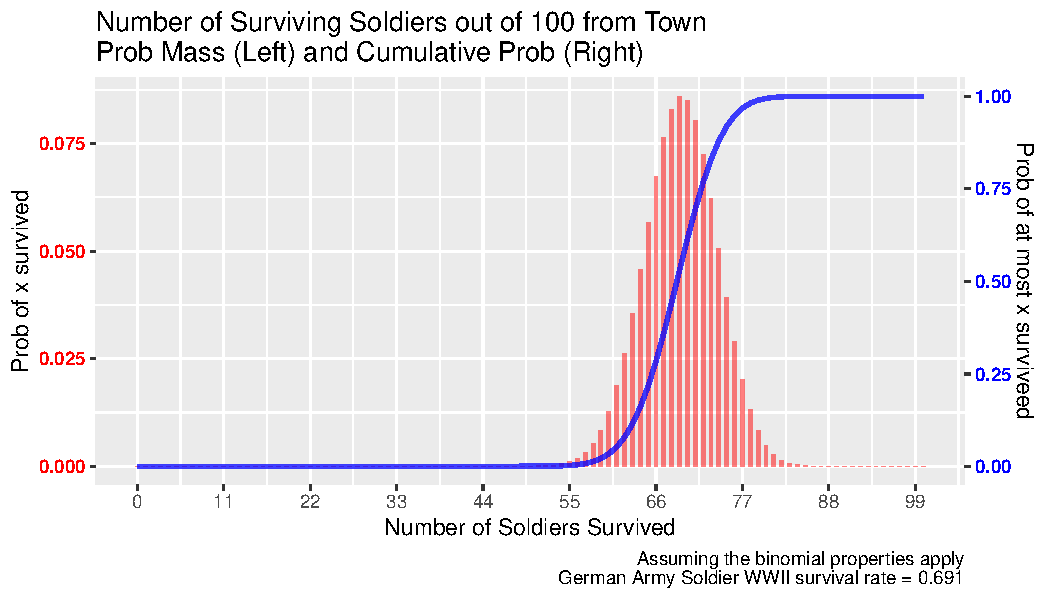
\includegraphics{Introductory-Statistics-with-R-tidyverse_files/figure-latex/unnamed-chunk-73-1} \end{center}

\hypertarget{wwii-german-soldiertable}{%
\subsubsection{WWII German Soldier--Table}\label{wwii-german-soldiertable}}

We can see from the table of results what is the distribution of the number of soldiers returning to each village in greater detail.

\begin{Shaded}
\begin{Highlighting}[]
\CommentTok{\# print(survive.prob)}
\CommentTok{\# start\_idx \textless{}{-} 81}
\NormalTok{f\_table \textless{}{-}}\StringTok{ }\ControlFlowTok{function}\NormalTok{(start\_idx) \{}

\NormalTok{    survive.subset \textless{}{-}}\StringTok{ }\KeywordTok{round}\NormalTok{(survive.prob[}\KeywordTok{seq}\NormalTok{(start\_idx, start\_idx}\OperatorTok{+}\DecValTok{20}\NormalTok{),], }\DecValTok{4}\NormalTok{)}
\NormalTok{    survive.subset}\OperatorTok{$}\NormalTok{prob \textless{}{-}}\StringTok{ }\KeywordTok{paste0}\NormalTok{(survive.subset}\OperatorTok{$}\NormalTok{prob}\OperatorTok{*}\DecValTok{100}\NormalTok{,}
                                  \StringTok{\textquotesingle{}\% chance EXACTLY (n=\textquotesingle{}}\NormalTok{, survive.subset}\OperatorTok{$}\NormalTok{survives, }\StringTok{\textquotesingle{}) survived\textquotesingle{}}\NormalTok{)}
\NormalTok{    survive.subset}\OperatorTok{$}\NormalTok{one.minus.cum.prob \textless{}{-}}\StringTok{ }\KeywordTok{paste0}\NormalTok{((}\DecValTok{1}\OperatorTok{{-}}\NormalTok{survive.subset}\OperatorTok{$}\NormalTok{cum.prob)}\OperatorTok{*}\DecValTok{100}\NormalTok{,}
                                                \StringTok{\textquotesingle{}\% chance AT LEAST (n=\textquotesingle{}}\NormalTok{, survive.subset}\OperatorTok{$}\NormalTok{survives, }\StringTok{\textquotesingle{}) survived\textquotesingle{}}\NormalTok{)}
\NormalTok{    survive.subset}\OperatorTok{$}\NormalTok{cum.prob \textless{}{-}}\StringTok{ }\KeywordTok{paste0}\NormalTok{(}\KeywordTok{round}\NormalTok{((survive.subset}\OperatorTok{$}\NormalTok{cum.prob)}\OperatorTok{*}\DecValTok{100}\NormalTok{, }\DecValTok{4}\NormalTok{),}
                                      \StringTok{\textquotesingle{}\% chance AT MOST (n=\textquotesingle{}}\NormalTok{, survive.subset}\OperatorTok{$}\NormalTok{survives, }\StringTok{\textquotesingle{}) survived\textquotesingle{}}\NormalTok{)}

    \KeywordTok{return}\NormalTok{(survive.subset[,}\DecValTok{2}\OperatorTok{:}\DecValTok{4}\NormalTok{])}
\NormalTok{\}}
\KeywordTok{lapply}\NormalTok{(}\KeywordTok{c}\NormalTok{(}\DecValTok{1}\NormalTok{,}\DecValTok{21}\NormalTok{,}\DecValTok{41}\NormalTok{,}\DecValTok{61}\NormalTok{,}\DecValTok{81}\NormalTok{), f\_table)}
\end{Highlighting}
\end{Shaded}

\begin{verbatim}
## [[1]]
## 
## [[2]]
## 
## [[3]]
## 
## [[4]]
## 
## [[5]]
\end{verbatim}

\hypertarget{poisson-distribution}{%
\section{Poisson Distribution}\label{poisson-distribution}}

\begin{quote}
Go back to \href{http://fanwangecon.github.io/}{fan}'s \href{https://fanwangecon.github.io/REconTools/}{REconTools} Package, \href{https://fanwangecon.github.io/R4Econ/}{R Code Examples} Repository (\href{https://fanwangecon.github.io/R4Econ/bookdown}{bookdown site}), or \href{https://fanwangecon.github.io/Stat4Econ/}{Intro Stats with R} Repository (\href{https://fanwangecon.github.io/Stat4Econ/bookdown}{bookdown site}).
\end{quote}

We looked at the binomial probability distribution \href{https://fanwangecon.github.io/Stat4Econ/probability/htmlpdfr/binomial.html}{Discrete Random Variable and Binomial Experiment}. Now we look at the poisson distribution.

Suppose you run a restaurant, maybe you know on average how many guests arrive on a weekday night between 6 and 9, but every night the exact number might be different, what is the distribution of guest arrivals? By chance, there could be \(0\) guests, there could also be a lot more guest than average potentially. We use the poisson distribution to think about these arrival probabilities.

For us to use the Poisson distribution, the experiment we study need to have these two properties (ASWCC P250):

\begin{enumerate}
\def\labelenumi{\arabic{enumi}.}
\tightlist
\item
  ``The probability of an occurrence is the same for any two intervals of equal length.''
\item
  ``The occurrence or nonoccurrence in any interval is independent of the occurrence or nonoccurrence in any other interval.''
\end{enumerate}

\textbf{Poisson Sample Space}

Guests arrive at your restaurant between 6 and 9 on a weekday night, 0 guest could arrive, 1, 2, 3, \ldots, 10, 11, 13, \ldots{} , 20, 21, 22, \ldots. Unlike in the Binomial case, where we have a maximum number of games that we can win out of \(n\) games played, here we don't impose a maximum number of guests that can arrive.

\begin{itemize}
\tightlist
\item
  Experiment: arrivals
\item
  Experimental outcomes: \(x=0,x=1,...,...\), unlike the bionomial, there is no limit here
\item
  Sample Space: \(S=\left\{0,1,...,...\right\}\) (the support is infinite)
\end{itemize}

\textbf{Poisson Probability Mass Funcion}

What is the probability of having \(x\) arrivals during an interval of time given that the expected (mean) number of arrival in that interval of time is \(\mu\)? The answer is given by this formula, which is the poisson probability mass function:

\begin{eqnarray}
f(x;\mu) &=& \frac{\mu^{x} \cdot e^{-\mu}}{x!}\\
\end{eqnarray}

With the poisson experiment, we have this formula to assign probabilities. The formula has two inputs, \(x\) and \(\mu\). \(e=2.71828\) is not a parameter, it is a fixed number like \(\pi\), it is a mathematical constant. You need to tell R, Excel, or alternative programs what these two numbers \(x\) and \(\mu\) are, and the program will spit a probability out for you. \(\mu\) is the parameter.

\textbf{Poisson Expected Value and Variance}

For the Poisson discrete random variable, it turns out the expected value and variance are:
\[E(x) = \mu\]
\[Var(x) = \mu\]

We can check by summing over : \(E(x) = \mu_x = \Sigma x \cdot f(x)\) and \(Var(x) = \sigma_x^2 = \Sigma \left( (x - \mu_x)^2 \cdot f(x) \right)\), and we will always end up with these two results. Note that if we are actually adding up terms, since there is no maximum arrival limit, we have to approximate the summation up to a large number of arrivals.

\hypertarget{poisson-example-horse-kicking}{%
\subsection{Poisson Example: Horse-Kicking}\label{poisson-example-horse-kicking}}

Using data from the \href{https://en.wikipedia.org/wiki/Prussian_Army}{Prussian Army} on ``number of soldiers killed by being kicked by a horse each year in each of 14 cavalry corps over a 20-year period'', \href{https://en.wikipedia.org/wiki/Ladislaus_Bortkiewicz}{Ladislaus Bortkiewicz} showed in 1898 in \href{https://de.wikipedia.org/wiki/Gesetz_der_kleinen_Zahlen}{Gesetz der kleinen Zahlen (The Rule of Small Numbers)} that this followed the Poisson distribution. This is one of the most famous examples of the Poisson Distribution.

He found that there was 0.70 deaths per one corps per one year.

\textbf{Chance of 2 death per year per corp}

\begin{itemize}
\tightlist
\item
  \(x=2\): 2 death in a corp in a year by horse-kick
\item
  \(\mu=0.70\)
\end{itemize}

For example, the chance that \(2\) soldier from a corp in a year die of horse kick:
\[f\left(x=2;\mu=0.7\right) = \frac{0.7^{2} \cdot e^{-0.7}}{2!} = 0.122\]

We can use the r function, \emph{dpois}, to calculate these probabilites: \emph{dpois(2, 0.7)}. Additionally, \emph{ppois(2,0.7)} calculates the cumulative probability that at most 2 die from horse-kick in a corp in a year.

\textbf{Distributional Graphs Horse Kicking Death Per Corp Per Year}

We can see from the results below that given our parameter \(\mu=0.7\), there is almost a 50 percent chance that a corp has no death from horse kick in a year. And the chances that 1, 2, 3 and 4 Prussian soldiers die from horse-kick are 35, 12, 3, and 0.5 percent.

The chance that at least 2 soldiers die from each corp each year is 16 percent.

If you are running the Prussian Army, you would want to know these statistics. You would want to track these statistics overtime and try to improve training etc.

\begin{Shaded}
\begin{Highlighting}[]
\KeywordTok{library}\NormalTok{(tidyverse)}

\CommentTok{\# Parameters}
\NormalTok{n \textless{}{-}}\StringTok{ }\DecValTok{10}
\NormalTok{mu \textless{}{-}}\StringTok{ }\FloatTok{0.70}

\CommentTok{\# Generate Data}
\CommentTok{\# A vector of different survival counts}
\NormalTok{zero2large \textless{}{-}}\StringTok{ }\DecValTok{0}\OperatorTok{:}\NormalTok{n}
\CommentTok{\# Probability for different survival counts}
\NormalTok{prob\_of\_diekicks \textless{}{-}}\StringTok{ }\KeywordTok{dpois}\NormalTok{(zero2large, mu)}
\CommentTok{\# Cumulative Probability for different survival counts, before dbinom, now pbinom}
\NormalTok{cumulative\_prob\_of\_diekicks \textless{}{-}}\StringTok{ }\KeywordTok{ppois}\NormalTok{(zero2large, mu)}
\CommentTok{\# Data File that Includes Cumulative Probability and Mass}
\NormalTok{diekick.prob \textless{}{-}}\StringTok{ }\KeywordTok{tibble}\NormalTok{(}\DataTypeTok{diekicks=}\NormalTok{(zero2large), }\DataTypeTok{prob=}\NormalTok{prob\_of\_diekicks, }\DataTypeTok{cum.prob=}\NormalTok{cumulative\_prob\_of\_diekicks)}

\CommentTok{\# Control Graph Size}
\KeywordTok{options}\NormalTok{(}\DataTypeTok{repr.plot.width =} \DecValTok{5}\NormalTok{, }\DataTypeTok{repr.plot.height =} \DecValTok{4}\NormalTok{)}
\CommentTok{\# Two axis colors}
\NormalTok{axis.sec.ratio \textless{}{-}}\StringTok{ }\KeywordTok{max}\NormalTok{(cumulative\_prob\_of\_diekicks)}\OperatorTok{/}\KeywordTok{max}\NormalTok{(prob\_of\_diekicks)}
\NormalTok{right.axis.color \textless{}{-}}\StringTok{ \textquotesingle{}blue\textquotesingle{}}
\NormalTok{left.axis.color \textless{}{-}}\StringTok{ \textquotesingle{}red\textquotesingle{}}

\CommentTok{\# Probabilities}
\NormalTok{diekick.graph \textless{}{-}}\StringTok{ }\NormalTok{diekick.prob }\OperatorTok{\%\textgreater{}\%}
\StringTok{    }\KeywordTok{ggplot}\NormalTok{(}\KeywordTok{aes}\NormalTok{(}\DataTypeTok{x=}\NormalTok{diekicks)) }\OperatorTok{+}
\StringTok{    }\KeywordTok{geom\_bar}\NormalTok{(}\KeywordTok{aes}\NormalTok{(}\DataTypeTok{y=}\NormalTok{prob),}
             \DataTypeTok{stat=}\StringTok{\textquotesingle{}identity\textquotesingle{}}\NormalTok{, }\DataTypeTok{alpha=}\FloatTok{0.5}\NormalTok{, }\DataTypeTok{width=}\FloatTok{0.5}\NormalTok{, }\DataTypeTok{fill=}\NormalTok{left.axis.color) }\OperatorTok{+}
\StringTok{    }\KeywordTok{geom\_text}\NormalTok{(}\KeywordTok{aes}\NormalTok{(}\DataTypeTok{y=}\NormalTok{prob,}
                  \DataTypeTok{label =} \KeywordTok{paste0}\NormalTok{(}\KeywordTok{sprintf}\NormalTok{(}\StringTok{\textquotesingle{}\%2.1f\textquotesingle{}}\NormalTok{, prob}\OperatorTok{*}\DecValTok{100}\NormalTok{), }\StringTok{\textquotesingle{}\%\textquotesingle{}}\NormalTok{)),}
              \DataTypeTok{vjust =} \FloatTok{{-}0.}\NormalTok{, }\DataTypeTok{size =} \DecValTok{3}\NormalTok{, }\DataTypeTok{color=}\NormalTok{left.axis.color, }\DataTypeTok{fontface=}\StringTok{\textquotesingle{}bold\textquotesingle{}}\NormalTok{)}

\CommentTok{\# Cumulative Probabilities}
\NormalTok{diekick.graph \textless{}{-}}\StringTok{ }\NormalTok{diekick.graph }\OperatorTok{+}
\StringTok{    }\KeywordTok{geom\_line}\NormalTok{(}\KeywordTok{aes}\NormalTok{(}\DataTypeTok{y=}\NormalTok{cum.prob}\OperatorTok{/}\NormalTok{axis.sec.ratio),}
              \DataTypeTok{alpha=}\FloatTok{0.25}\NormalTok{, }\DataTypeTok{size=}\DecValTok{1}\NormalTok{, }\DataTypeTok{color=}\NormalTok{right.axis.color) }\OperatorTok{+}
\StringTok{    }\KeywordTok{geom\_point}\NormalTok{(}\KeywordTok{aes}\NormalTok{(}\DataTypeTok{y=}\NormalTok{cum.prob}\OperatorTok{/}\NormalTok{axis.sec.ratio),}
               \DataTypeTok{alpha=}\FloatTok{0.75}\NormalTok{, }\DataTypeTok{size=}\DecValTok{2}\NormalTok{, }\DataTypeTok{shape=}\DecValTok{23}\NormalTok{, }\DataTypeTok{fill=}\NormalTok{right.axis.color) }\OperatorTok{+}
\StringTok{    }\KeywordTok{geom\_text}\NormalTok{(}\KeywordTok{aes}\NormalTok{(}\DataTypeTok{y=}\NormalTok{cum.prob}\OperatorTok{/}\NormalTok{axis.sec.ratio,}
                  \DataTypeTok{label =} \KeywordTok{paste0}\NormalTok{(}\KeywordTok{sprintf}\NormalTok{(}\StringTok{\textquotesingle{}\%2.0f\textquotesingle{}}\NormalTok{, cum.prob}\OperatorTok{*}\DecValTok{100}\NormalTok{), }\StringTok{\textquotesingle{}\%\textquotesingle{}}\NormalTok{)),}
              \DataTypeTok{vjust =} \FloatTok{{-}0.5}\NormalTok{, }\DataTypeTok{size =} \DecValTok{3}\NormalTok{, }\DataTypeTok{color=}\NormalTok{right.axis.color, }\DataTypeTok{fontface=}\StringTok{\textquotesingle{}bold\textquotesingle{}}\NormalTok{)}


\CommentTok{\# Graph Strings}
\NormalTok{graph.title \textless{}{-}}\StringTok{ }\KeywordTok{sprintf}\NormalTok{(}
    \KeywordTok{paste0}\NormalTok{(}\StringTok{\textquotesingle{}Death from Horse Kick Per Corp Per Year}\CharTok{\textbackslash{}n}\StringTok{\textquotesingle{}}\NormalTok{,}
           \StringTok{\textquotesingle{}Prob Mass (Left) and Cumulative Prob (Right)\textquotesingle{}}\NormalTok{))}
\NormalTok{graph.caption \textless{}{-}}\StringTok{ }\KeywordTok{sprintf}\NormalTok{(}
    \KeywordTok{paste0}\NormalTok{(}\StringTok{\textquotesingle{}Assuming the Poisson properties apply}\CharTok{\textbackslash{}n}\StringTok{\textquotesingle{}}\NormalTok{,}
           \StringTok{\textquotesingle{}Ladislaus Bortkiewicz Prussian Data}\CharTok{\textbackslash{}n}\StringTok{\textquotesingle{}}\NormalTok{,}
           \StringTok{\textquotesingle{}Death By Horse Kick Per Corp Per Year = \%s\textquotesingle{}}\NormalTok{), mu)}
\NormalTok{graph.title.x \textless{}{-}}\StringTok{ \textquotesingle{}Number of Soldiers Die of Horse Kick\textquotesingle{}}
\NormalTok{graph.title.y.axisleft \textless{}{-}}\StringTok{ \textquotesingle{}Prob of x Die of Horse Kick\textquotesingle{}}
\NormalTok{graph.title.y.axisright \textless{}{-}}\StringTok{ \textquotesingle{}Prob of at Most x Die Of Horse Kick\textquotesingle{}}

\CommentTok{\# Graphing}
\NormalTok{diekick.graph \textless{}{-}}\StringTok{ }\NormalTok{diekick.graph }\OperatorTok{+}
\StringTok{    }\KeywordTok{labs}\NormalTok{(}\DataTypeTok{title =}\NormalTok{ graph.title,}
         \DataTypeTok{x =}\NormalTok{ graph.title.x,}
         \DataTypeTok{y =}\NormalTok{ graph.title.y.axisleft,}
         \DataTypeTok{caption =}\NormalTok{ graph.caption) }\OperatorTok{+}
\StringTok{    }\KeywordTok{scale\_y\_continuous}\NormalTok{(}\DataTypeTok{sec.axis =}
                       \KeywordTok{sec\_axis}\NormalTok{(}\OperatorTok{\textasciitilde{}}\NormalTok{.}\OperatorTok{*}\NormalTok{axis.sec.ratio,}
                                \DataTypeTok{name =}\NormalTok{ graph.title.y.axisright)) }\OperatorTok{+}
\StringTok{    }\KeywordTok{scale\_x\_continuous}\NormalTok{(}\DataTypeTok{labels =}\NormalTok{ zero2large[}\KeywordTok{floor}\NormalTok{(}\KeywordTok{seq}\NormalTok{(}\DecValTok{1}\NormalTok{,n,}\DataTypeTok{length.out=}\DecValTok{10}\NormalTok{))],}
                       \DataTypeTok{breaks =}\NormalTok{ zero2large[}\KeywordTok{floor}\NormalTok{(}\KeywordTok{seq}\NormalTok{(}\DecValTok{1}\NormalTok{,n,}\DataTypeTok{length.out=}\DecValTok{10}\NormalTok{))]) }\OperatorTok{+}
\StringTok{    }\KeywordTok{theme}\NormalTok{(}\DataTypeTok{axis.text.y =} \KeywordTok{element\_text}\NormalTok{(}\DataTypeTok{face=}\StringTok{\textquotesingle{}bold\textquotesingle{}}\NormalTok{),}
          \DataTypeTok{axis.text.y.right =} \KeywordTok{element\_text}\NormalTok{(}\DataTypeTok{color =}\NormalTok{ right.axis.color),}
          \DataTypeTok{axis.text.y.left =} \KeywordTok{element\_text}\NormalTok{(}\DataTypeTok{color =}\NormalTok{ left.axis.color))}

\CommentTok{\# Print}
\KeywordTok{print}\NormalTok{(diekick.graph)}
\end{Highlighting}
\end{Shaded}

\begin{center}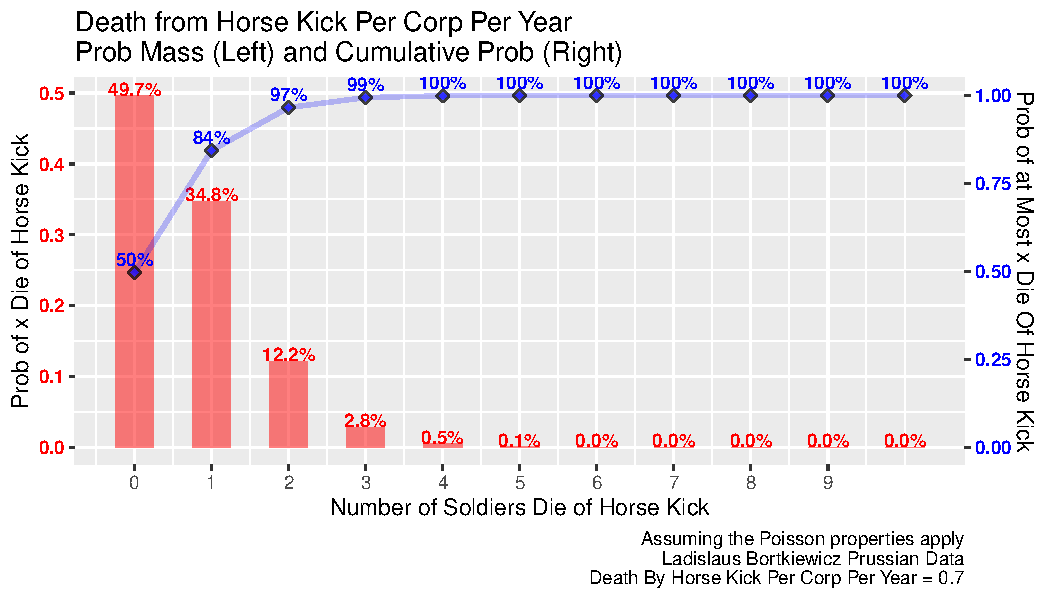
\includegraphics{Introductory-Statistics-with-R-tidyverse_files/figure-latex/unnamed-chunk-76-1} \end{center}

\begin{Shaded}
\begin{Highlighting}[]
\CommentTok{\# Tabular}
\KeywordTok{round}\NormalTok{(}\KeywordTok{as.tibble}\NormalTok{(diekick.prob), }\DecValTok{3}\NormalTok{)}
\end{Highlighting}
\end{Shaded}

\hypertarget{appendix-appendix}{%
\appendix}


\hypertarget{index-and-code-links}{%
\chapter{Index and Code Links}\label{index-and-code-links}}

\hypertarget{survey-links}{%
\section{Survey links}\label{survey-links}}

\begin{enumerate}
\def\labelenumi{\arabic{enumi}.}
\tightlist
\item
  \href{https://fanwangecon.github.io/Stat4Econ/survey/htmlpdfr/classsurvey.html}{An In-class Survey}: \href{https://github.com/FanWangEcon/Stat4Econ/blob/master/survey//classsurvey.Rmd}{\textbf{rmd}} \textbar{} \href{https://github.com/FanWangEcon/Stat4Econ/blob/master/survey/htmlpdfr/classsurvey.R}{\textbf{r}} \textbar{} \href{https://github.com/FanWangEcon/Stat4Econ/blob/master/survey/htmlpdfr/classsurvey.pdf}{\textbf{pdf}} \textbar{} \href{https://fanwangecon.github.io/Stat4Econ/survey/htmlpdfr/classsurvey.html}{\textbf{html}}

  \begin{itemize}
  \tightlist
  \item
    create a tibble dataset
  \item
    draw 10 random students from 50 and build a survey
  \item
    \textbf{r}: \emph{factor() + ifelse()}
  \item
    \textbf{dplyr}: \emph{group\_by() + mutate() + summarise()}
  \item
    \textbf{tibble}: \emph{add\_row()}
  \item
    \textbf{readr}: \emph{write\_csv()}
  \end{itemize}
\end{enumerate}

\hypertarget{dataset-tables-and-graphs-links}{%
\section{Dataset, Tables and Graphs links}\label{dataset-tables-and-graphs-links}}

\begin{enumerate}
\def\labelenumi{\arabic{enumi}.}
\tightlist
\item
  \href{https://fanwangecon.github.io/Stat4Econ/descriptive/htmlpdfr/DataBasketball.html}{Opening a Dataset}: \href{https://github.com/FanWangEcon/Stat4Econ/blob/master/descriptive//DataBasketball.Rmd}{\textbf{rmd}} \textbar{} \href{https://github.com/FanWangEcon/Stat4Econ/blob/master/descriptive/htmlpdfr/DataBasketball.R}{\textbf{r}} \textbar{} \href{https://github.com/FanWangEcon/Stat4Econ/blob/master/descriptive/htmlpdfr/DataBasketball.pdf}{\textbf{pdf}} \textbar{} \href{https://fanwangecon.github.io/Stat4Econ/descriptive/htmlpdfr/DataBasketball.html}{\textbf{html}}

  \begin{itemize}
  \tightlist
  \item
    Opening a Dataset.
  \item
    \textbf{r}: \emph{setwd()}
  \item
    \textbf{readr}: \emph{write\_csv()}
  \end{itemize}
\item
  \href{https://fanwangecon.github.io/Stat4Econ/descriptive/htmlpdfr/OneVariable.html}{One Variable Graphs and Tables}: \href{https://github.com/FanWangEcon/Stat4Econ/blob/master/descriptive//OneVariable.Rmd}{\textbf{rmd}} \textbar{} \href{https://github.com/FanWangEcon/Stat4Econ/blob/master/descriptive/htmlpdfr/OneVariable.R}{\textbf{r}} \textbar{} \href{https://github.com/FanWangEcon/Stat4Econ/blob/master/descriptive/htmlpdfr/OneVariable.pdf}{\textbf{pdf}} \textbar{} \href{https://fanwangecon.github.io/Stat4Econ/descriptive/htmlpdfr/OneVariable.html}{\textbf{html}}

  \begin{itemize}
  \tightlist
  \item
    Frequency table, bar chart and histogram.
  \item
    R function and lapply to generate graphs/tables for different variables.
  \item
    \textbf{r}: \emph{c(`word1',`word2') + function() + for (ctr in c(1,2)) \{\} + lapply()}
  \item
    \textbf{dplyr}: \emph{group\_by() + summarize() + n()}
  \item
    \textbf{ggplot}: \emph{geom\_bar() + geom\_histogram() + labs(title = `title', caption = `caption')}
  \end{itemize}
\item
  \href{https://fanwangecon.github.io/Stat4Econ/descriptive/htmlpdfr/MultipleVariables.html}{Multiple Variables Graphs and Tables}: \href{https://github.com/FanWangEcon/Stat4Econ/blob/master/descriptive//MultipleVariables.Rmd}{\textbf{rmd}} \textbar{} \href{https://github.com/FanWangEcon/Stat4Econ/blob/master/descriptive/htmlpdfr/MultipleVariables.R}{\textbf{r}} \textbar{} \href{https://github.com/FanWangEcon/Stat4Econ/blob/master/descriptive/htmlpdfr/MultipleVariables.pdf}{\textbf{pdf}} \textbar{} \href{https://fanwangecon.github.io/Stat4Econ/descriptive/htmlpdfr/MultipleVariables.html}{\textbf{html}}

  \begin{itemize}
  \tightlist
  \item
    Two-way frequency table, stacked bar chart annd scatter-plot
  \item
    \textbf{r}: \emph{interaction()}
  \item
    \textbf{dplyr}: \emph{group\_by(var) + summarize(freq = n()) + spread(gender, freq)}
  \item
    \textbf{ggplot}: \emph{aes(x,y,fill) + geom\_bar(stat=`identity', fun.y=`mean', position=`dodge') + geom\_point(size) + geom\_text(size,hjust,vjust) + geom\_smooth(method=lm) + labs(title,x,y,caption)}
  \end{itemize}
\end{enumerate}

\hypertarget{summarizing-data-links}{%
\section{Summarizing Data links}\label{summarizing-data-links}}

\begin{enumerate}
\def\labelenumi{\arabic{enumi}.}
\tightlist
\item
  \href{https://fanwangecon.github.io/Stat4Econ/summarystats/htmlpdfr/meansdhist.html}{Mean and Standard Deviation}: \href{https://github.com/FanWangEcon/Stat4Econ/blob/master/summarystats//meansdhist.Rmd}{\textbf{rmd}} \textbar{} \href{https://github.com/FanWangEcon/Stat4Econ/blob/master/summarystats/htmlpdfr/meansdhist.R}{\textbf{r}} \textbar{} \href{https://github.com/FanWangEcon/Stat4Econ/blob/master/summarystats/htmlpdfr/meansdhist.pdf}{\textbf{pdf}} \textbar{} \href{https://fanwangecon.github.io/Stat4Econ/summarystats/htmlpdfr/meansdhist.html}{\textbf{html}}

  \begin{itemize}
  \tightlist
  \item
    Mean and standard deviation from a dataset with city-month temperatures.
  \item
    \textbf{r}: \emph{dim() + min() + ceiling() + lapply() + vector(mode=``character'',length) + substring(var, first, last) + func \textless- function(return(list))}
  \item
    \textbf{dplyr}: \emph{mutate() + select() + filter()}
  \item
    \textbf{tidyr}: \emph{gather(vara, val, -varb)}
  \item
    \textbf{rlang}: \emph{!!sym(str\_var\_name)}
  \item
    \textbf{ggplot}: \emph{aes(x, y, colour, linetype, shape) + facet\_wrap(\textasciitilde var, scales=`free\_y') + geom\_line() + geom\_point() + geom\_jitter(size, width) + scale\_x\_continuous(labels, breaks)}
  \end{itemize}
\item
  \href{https://fanwangecon.github.io/Stat4Econ/summarystats/htmlpdfr/toolboxone.html}{Rescaling Standard Deviation and Covariance}: \href{https://github.com/FanWangEcon/Stat4Econ/blob/master/summarystats//toolboxone.Rmd}{\textbf{rmd}} \textbar{} \href{https://github.com/FanWangEcon/Stat4Econ/blob/master/summarystats/htmlpdfr/toolboxone.R}{\textbf{r}} \textbar{} \href{https://github.com/FanWangEcon/Stat4Econ/blob/master/summarystats/htmlpdfr/toolboxone.pdf}{\textbf{pdf}} \textbar{} \href{https://fanwangecon.github.io/Stat4Econ/summarystats/htmlpdfr/toolboxone.html}{\textbf{html}}

  \begin{itemize}
  \tightlist
  \item
    Scatter-plot of a dataset with state-level wage and education data.
  \item
    Coefficient of variation and standard deviation, correlation and covariance.
  \item
    \textbf{r}: \emph{mean() + sd() + var() + cov() + cor()}
  \item
    \textbf{ggplot}: \emph{geom\_point(size) + geom\_text() + geom\_smooth()}
  \end{itemize}
\end{enumerate}

\hypertarget{basics-of-probability-links}{%
\section{Basics of Probability links}\label{basics-of-probability-links}}

\begin{enumerate}
\def\labelenumi{\arabic{enumi}.}
\tightlist
\item
  \href{https://fanwangecon.github.io/Stat4Econ/probability/htmlpdfr/samplespace.html}{Sample Space, Experimental Outcomes, Events, Probabilities}: \href{https://github.com/FanWangEcon/Stat4Econ/blob/master/probability//samplespace.Rmd}{\textbf{rmd}} \textbar{} \href{https://github.com/FanWangEcon/Stat4Econ/blob/master/probability/htmlpdfr/samplespace.R}{\textbf{r}} \textbar{} \href{https://github.com/FanWangEcon/Stat4Econ/blob/master/probability/htmlpdfr/samplespace.pdf}{\textbf{pdf}} \textbar{} \href{https://fanwangecon.github.io/Stat4Econ/probability/htmlpdfr/samplespace.html}{\textbf{html}}

  \begin{itemize}
  \tightlist
  \item
    Sample Space, Experimental Outcomes, Events and Probability.
  \item
    Union, intersection and complements
  \item
    conditional probability
  \end{itemize}
\item
  \href{https://fanwangecon.github.io/Stat4Econ/probability/htmlpdfr/samplespaceexa.html}{Examples of Sample Space and Probabilities}: \href{https://github.com/FanWangEcon/Stat4Econ/blob/master/probability//samplespaceexa.Rmd}{\textbf{rmd}} \textbar{} \href{https://github.com/FanWangEcon/Stat4Econ/blob/master/probability/htmlpdfr/samplespaceexa.R}{\textbf{r}} \textbar{} \href{https://github.com/FanWangEcon/Stat4Econ/blob/master/probability/htmlpdfr/samplespaceexa.pdf}{\textbf{pdf}} \textbar{} \href{https://fanwangecon.github.io/Stat4Econ/probability/htmlpdfr/samplespaceexa.html}{\textbf{html}}

  \begin{itemize}
  \tightlist
  \item
    Throwing a quarter, four candidates for election, six-sided unfair dice, two basketball games
  \item
    \textbf{r}: \emph{sample(size, replace, prob)}
  \end{itemize}
\item
  \href{https://fanwangecon.github.io/Stat4Econ/probability/htmlpdfr/samplespacedice.html}{Throw an Unfair Four Sided Dice}: \href{https://github.com/FanWangEcon/Stat4Econ/blob/master/probability//samplespacedice.Rmd}{\textbf{rmd}} \textbar{} \href{https://github.com/FanWangEcon/Stat4Econ/blob/master/probability/htmlpdfr/samplespacedice.R}{\textbf{r}} \textbar{} \href{https://github.com/FanWangEcon/Stat4Econ/blob/master/probability/htmlpdfr/samplespacedice.pdf}{\textbf{pdf}} \textbar{} \href{https://fanwangecon.github.io/Stat4Econ/probability/htmlpdfr/samplespacedice.html}{\textbf{html}}

  \begin{itemize}
  \tightlist
  \item
    Throw an unfair dice many times, law of large number.
  \item
    \textbf{r}: \emph{head() + tail() + factor() + sample() + as.numeric() + paste0(`dice=', var) + sprintf(`\%0.3f', 1.1234) + sprintf(``P(S=1)=\%0.3f, P(S=2)=\%0.3f'', 1.1, 1.2345)}
  \item
    \textbf{stringr}: \emph{str\_extract() + as.numeric(str\_extract(variable, ``{[}\^{}.n{]}+\$'')))}
  \item
    \textbf{dplyr}: \emph{mutate(!!str\_mean\_var := as.numeric(sprintf(`\%0.5f', freq / sum(freq))))}
  \item
    \textbf{ggplot}: \emph{geom\_line() + scale\_x\_continuous(trans=`log10', labels=c(`n=100', `n=1000'), breaks=c(100, 1000))}
  \end{itemize}
\item
  \href{https://fanwangecon.github.io/Stat4Econ/probability/htmlpdfr/lottery.html}{Multiple-Step Experiment: Playing the Lottery Three times}: \href{https://github.com/FanWangEcon/Stat4Econ/blob/master/probability//lottery.Rmd}{\textbf{rmd}} \textbar{} \href{https://github.com/FanWangEcon/Stat4Econ/blob/master/probability/htmlpdfr/lottery.R}{\textbf{r}} \textbar{} \href{https://github.com/FanWangEcon/Stat4Econ/blob/master/probability/htmlpdfr/lottery.pdf}{\textbf{pdf}} \textbar{} \href{https://fanwangecon.github.io/Stat4Econ/probability/htmlpdfr/lottery.html}{\textbf{html}}

  \begin{itemize}
  \tightlist
  \item
    Paths after 1, 2 and 3 plays.
  \end{itemize}
\end{enumerate}

\hypertarget{discrete-probability-distribution-links}{%
\section{Discrete Probability Distribution links}\label{discrete-probability-distribution-links}}

\begin{enumerate}
\def\labelenumi{\arabic{enumi}.}
\tightlist
\item
  \href{https://fanwangecon.github.io/Stat4Econ/probability_discrete/htmlpdfr/binomial.html}{Discrete Random Variable and Binomial Experiment}: \href{https://github.com/FanWangEcon/Stat4Econ/blob/master/probability_discrete//binomial.Rmd}{\textbf{rmd}} \textbar{} \href{https://github.com/FanWangEcon/Stat4Econ/blob/master/probability_discrete/htmlpdfr/binomial.R}{\textbf{r}} \textbar{} \href{https://github.com/FanWangEcon/Stat4Econ/blob/master/probability_discrete/htmlpdfr/binomial.pdf}{\textbf{pdf}} \textbar{} \href{https://fanwangecon.github.io/Stat4Econ/probability_discrete/htmlpdfr/binomial.html}{\textbf{html}}

  \begin{itemize}
  \tightlist
  \item
    Discrete Random Variable, expected value and variance.
  \item
    Binomial Properties, examples using USA larceny clearance rate, WWII German soldier survival rate
  \item
    \textbf{r}: \emph{dbinom() + pbinom() + sprintf(paste0(`abc\textbackslash n', `efg = \%s'), `opq') + round(1.123, 2) + lapply()}
  \item
    \textbf{ggplot}: \emph{df \%\textgreater\% ggplot(aes(x)) + geom\_bar(aes(y=prob), stat=`identity', alpha=0.5, width=0.5, fill) + geom\_text(aes(y=prob, label=paste0(sprintf(`\%2.1f', p), `\%')), vjust, size, color, fontface) + labs(title, x, y, caption) + scale\_y\_continuous(sec.axis, name) + + scale\_x\_continuous(labels, breaks) + theme(axis.text.y, axis.text.y.right, axis.text.y.left)}
  \end{itemize}
\item
  \href{https://fanwangecon.github.io/Stat4Econ/probability_discrete/htmlpdfr/poisson.html}{Poisson Probability Distribution}: \href{https://github.com/FanWangEcon/Stat4Econ/blob/master/probability_discrete//poisson.Rmd}{\textbf{rmd}} \textbar{} \href{https://github.com/FanWangEcon/Stat4Econ/blob/master/probability_discrete/htmlpdfr/poisson.R}{\textbf{r}} \textbar{} \href{https://github.com/FanWangEcon/Stat4Econ/blob/master/probability_discrete/htmlpdfr/poisson.pdf}{\textbf{pdf}} \textbar{} \href{https://fanwangecon.github.io/Stat4Econ/probability_discrete/htmlpdfr/poisson.html}{\textbf{html}}

  \begin{itemize}
  \tightlist
  \item
    Poisson Properties, Ladislaus Bortkiewicz and Prussian army horse-kick deaths.
  \item
    \textbf{r}: \emph{dpois() + ppois()}
  \item
    \textbf{ggplot}: \emph{geom\_bar() + geom\_text() + gome\_line() + geom\_point() + geom\_text() + labs() + scale\_y\_continuous() + scale\_x\_continuous() + theme()}
  \end{itemize}
\end{enumerate}

  \bibliography{book.bib,packages.bib}

\end{document}
